%%%%%%%%%%%%%%%%%%%%%%%%%%%%%%%%%%%%%%%%%%%%%%%%%%%%%%%%%%%%%%%%%%%%%%%%%%%%%%%
% Titel:   Bericht - Admin
% Autoren: gross10
% Datum:   04.01.2014
% Version: 1.0.0
%%%%%%%%%%%%%%%%%%%%%%%%%%%%%%%%%%%%%%%%%%%%%%%%%%%%%%%%%%%%%%%%%%%%%%%%%%%%%%%
%
%:::Change-Log:::
% Versionierung erfolgt auf folgende Gegebenheiten: -1. Release Versionen
%                                                   -2. Neue Kapitel
%                                                   -3. Fehlerkorrekturen
%
% 0.0.1       Erstellung der Datei
%
%:::Hinweis:::
% Indexerstellung: makeindex -s report.ist report.idx
%   Umlaute m�ssen separat behandelt werden!
%%%%%%%%%%%%%%%%%%%%%%%%%%%%%%%%%%%%%%%%%%%%%%%%%%%%%%%%%%%%%%%%%%%%%%%%%%%%%%%
\documentclass[version=last,fleqn,pointlessnumbers,openright,twoside]{scrreprt}  %first: Ergebniss Kompatibel zu ersten Version; last: Ergebniss entspricht den aktuellen Paketen; fleqn: Formeln linksb�ndig; pointlessnumbers: Kapitelnummerierung ohne Punkt; twoside: Doppelseitiger Druck

%Dokumentangaben
\newcommand{\Titel}{Dokumentation PA2}
\newcommand{\Uebertitel}{Eurobot 2014 Kernteam}
\newcommand{\AutorA}{Hannes Roth}
\newcommand{\AutorB}{Patrick Rohrbach}
\newcommand{\AutorC}{Jascha Haldemann}
\newcommand{\AutorD}{Nicola K\"aser}
\newcommand{\AutorE}{Simon Grossenbacher}
\newcommand{\DozentA}{Daniel Lanz}
\newcommand{\DozentB}{Ivo Oesch}
\newcommand{\DozentC}{Walter G�ller}
\newcommand{\DozentD}{Roland Brun}
\newcommand{\FachbereichA}{Maschinenbau}
\newcommand{\FachbereichB}{Technik und Informatik}
\newcommand{\Datum}{\the\day.\the\month.\the\year}
\newcommand{\Ort}{Burgdorf}
\newcommand{\Version}{1.0.0}



%%%%%%%%%%%%%%%%%%%%%%%%%%%%%%%%%%%%%%%%%%%%%%%%%%%%%%%%%%%%%%%%%%%%%%%%%%%%%%%
% Pakete
%%%%%%%%%%%%%%%%%%%%%%%%%%%%%%%%%%%%%%%%%%%%%%%%%%%%%%%%%%%%%%%%%%%%%%%%%%%%%%%
%%%%%%%%%%%%%%%%%%%%%%%%%%%%%%%%%%%%%%%%%%%%%%%%%%%%%%%%%%%%%%%%%%%%%%%%%%%%%%%
% Titel:   Bericht - Pakete
% Autor: Simon Grossenbacher  
% Datum:   27.09.2013
% Version: 1.0.0
%%%%%%%%%%%%%%%%%%%%%%%%%%%%%%%%%%%%%%%%%%%%%%%%%%%%%%%%%%%%%%%%%%%%%%%%%%%%%%%
%
%:::Change-Log:::
% Versionierung erfolgt auf folgende Gegebenheiten: -1. Release Versionen
%                                                   -2. Neue Kapitel
%                                                   -3. Fehlerkorrekturen
%
% 0.0.0       Erstellung der Datei
%
%:::Hinweis:::
% Indexerstellung: makeindex -s report.ist report.idx
%   Umlaute m�ssen separat behandelt werden!
%%%%%%%%%%%%%%%%%%%%%%%%%%%%%%%%%%%%%%%%%%%%%%%%%%%%%%%%%%%%%%%%%%%%%%%%%%%%%%%

%Sprach-Optionen
\usepackage[ngerman]{babel} %neue deutsche Rechtschreibung
\usepackage[T1]{fontenc}  %richtige Worttrennung
%\usepackage[applemac]{inputenc}				% Mac - load extended character set (ISO 8859-1)
\usepackage[latin1]{inputenc}  				% Unix/Linux - load extended character set (ISO 8859-1)
%\usepackage[ansinew]{inputenc}  				% Windows - load extended character set (ISO 8859-1)
%\usepackage[utf8]{inputenc}  					% UTF-8 encoding

%Zeilenabstand
\usepackage{setspace}

%Mehr Tabellenoptionen
\usepackage{tabularx}
\usepackage{longtable}
\usepackage{rotating}
\usepackage{multirow}

%Listen
\usepackage{enumitem}

%Besserer Flattersatz
\usepackage{ragged2e}

%Gleiten verhindern
\usepackage{float}
\usepackage{placeins}

%Ueberschriften anpassen
\usepackage{titlesec} 

%Farben
\usepackage{color}
\usepackage{colortbl} %F�r farbige Tabellen

%PDF zu Dokument hinzufuegen
\usepackage[final]{pdfpages}

%Grafiken verwalten
\usepackage{graphicx}
\usepackage[absolute]{textpos}
\usepackage{wrapfig}
\usepackage{subcaption}

%Zeichnen
%\usepackage{pst-pdf}
%\usepackage{pst-all}

%Listnings verwalten
\usepackage{listings}

%Kopf- Fusszeile (Optionen m�ssen direkt �bergeben werden)
\usepackage[automark, %Automatisches aktualisieren der Chapter-Titel
%            headsepline,  %Linie Kopfzeile
%            footsepline,  %Linie fusszeilezeile
%            markuppercase,
            plainfootsepline  %Plain-Style auch mit Linie versehen
            ]{scrpage2}

%Flexible Argumente bei Funktionen
\usepackage{xargs}

%erweiterte Steuerfunktionen
\usepackage{ifthen}

%Index f�r Stichwortverzeichnis
\usepackage{makeidx}

%Index f�r Literaturverzeichnis
\usepackage[babel,german=quotes]{csquotes}
%\usepackage[backend=biber,style=numeric,defernumbers=true,sorting=nyt]{biblatex}
\usepackage[backend=bibtex,defernumbers=true]{biblatex}
\bibliography{bibliography}
\defbibheading{lit}{\section{Literatur}}
\defbibheading{pic}{\section{Abbildungen}}

%Zusaetzliche Symbole direkt im Text
\usepackage{textcomp}
\usepackage{amssymb}

%Einheit kontrolliert eingeben
\usepackage{units}

%dynamische Datumsausgabe
\usepackage[german]{isodate}

%Zusaetzlich Mathemtiksymbole
\usepackage{amsmath}
\usepackage{mathtools}

%Besser Handling von internen Countern und Berechnungen
\usepackage{calc}

%TODOs anbringen am Rand
\usepackage{todonotes}

%Hyperlinks (Muss das letzte geladene Paket sein)
\usepackage[bookmarks=true, %Verzeichnis generieren
            bookmarksopen=true, %Verzeichnis �ffnen
            bookmarksopenlevel=3, %Tiefe der Verzeichnis�ffnung
            unicode=false, %non-Latin Zeichen
            pdftoolbar=true, %PDF-Viewer Toolbar
            pdfmenubar=true, %PDF-Viewer Men�?
            pdffitwindow=true, %Fenster an Seite anpassen beim �ffnen
            pdftitle={\Titel}, %Titel
            %pdfauthor={\Autor1, \Autor2, \Autor3}, %Autor
            pdfsubject={\Uebertitel}, %Thema
%            pdfcreator={\Autor1, \Autor2, \Autor3}, %Ersteller des Dokuments
%            pdfproducer={\Autor1, \Autor2 \Autor3}, %Produzent des Dokuments
            pdfnewwindow=true, %Links in neuem Fenster
            colorlinks=true, %false: Boxen-Links; true: Farben-Links
            linkcolor=red, %Farbe von internen Links
            citecolor=red, %Farbe von Links zu Bibliography
            filecolor=magenta, %Farbe von Links zu Dateien
            urlcolor=blue %Farbe von externen Links
            ]{hyperref}
   
%Querverweise
\usepackage[german]{cleveref}
\usepackage{xr}  %Verweise uber Dokument hinweg

%Besseres Zeichensetzen
\usepackage{microtype}
            
%Glossar/Abk�rzungsverzeichnis
\usepackage[acronym,makeindex]{glossaries}




%%%%%%%%%%%%%%%%%%%%%%%%%%%%%%%%%%%%%%%%%%%%%%%%%%%%%%%%%%%%%%%%%%%%%%%%%%%%%%%
% Funktionen
%%%%%%%%%%%%%%%%%%%%%%%%%%%%%%%%%%%%%%%%%%%%%%%%%%%%%%%%%%%%%%%%%%%%%%%%%%%%%%%
%%%%%%%%%%%%%%%%%%%%%%%%%%%%%%%%%%%%%%%%%%%%%%%%%%%%%%%%%%%%%%%%%%%%%%%%%%%%%%%
% Titel:   Bericht - Funktionen
% Autor:   Simon Grossenbacher  
% Datum:   27.09.2013
% Version: 1.0.0
%%%%%%%%%%%%%%%%%%%%%%%%%%%%%%%%%%%%%%%%%%%%%%%%%%%%%%%%%%%%%%%%%%%%%%%%%%%%%%%
%
%:::Change-Log:::
% Versionierung erfolgt auf folgende Gegebenheiten: -1. Release Versionen
%                                                   -2. Neue Kapitel
%                                                   -3. Fehlerkorrekturen
%
% 0.0.0       Erstellung der Datei
%
%:::Hinweis:::
% Indexerstellung: makeindex -s report.ist report.idx
%   Umlaute m�ssen separat behandelt werden!
%%%%%%%%%%%%%%%%%%%%%%%%%%%%%%%%%%%%%%%%%%%%%%%%%%%%%%%%%%%%%%%%%%%%%%%%%%%%%%%

%%%%%%%%%%%%%%%%%%%%%%%%%%%%%%%%%%%%%%%%%%%%%%%%%%%%%%%%%%%%%%%%%%%%%%%%%%%%%%%
% Text tiefstellen
% param #1 Text
%%%%%%%%%%%%%%%%%%%%%%%%%%%%%%%%%%%%%%%%%%%%%%%%%%%%%%%%%%%%%%%%%%%%%%%%%%%%%%%
\newcommand{\low}[1]{\textsubscript{#1}}



%%%%%%%%%%%%%%%%%%%%%%%%%%%%%%%%%%%%%%%%%%%%%%%%%%%%%%%%%%%%%%%%%%%%%%%%%%%%%%%
% Text hochstellen
% param #1 Text
%%%%%%%%%%%%%%%%%%%%%%%%%%%%%%%%%%%%%%%%%%%%%%%%%%%%%%%%%%%%%%%%%%%%%%%%%%%%%%%
\newcommand{\high}[1]{\textsuperscript{#1}}



%%%%%%%%%%%%%%%%%%%%%%%%%%%%%%%%%%%%%%%%%%%%%%%%%%%%%%%%%%%%%%%%%%%%%%%%%%%%%%%
% Schrift anpassen
% param #1 Schriftfamilie: ptm  Times
%                          phv 	Helvetica
%                          pcr 	Courier
%                          pbk 	Bookman
%                          pag 	Avant Garde
%                          ppl 	Palatino
%                          pch 	Charter
%                          pnc 	New Century Schoolbook
%                          put 	Utopia
% param #2 Strichdicke/Zeichenbreite: b  bold
%                                     m  medium
% param #3 Schriftform: n   normal
%                       it  italic
%                       sl  slanted
%                       sc  small caps
%                       ui  upright italic
% note {\changefont{#1}{#2}{#3} Hallo Welt} Teilbereich aendern
%%%%%%%%%%%%%%%%%%%%%%%%%%%%%%%%%%%%%%%%%%%%%%%%%%%%%%%%%%%%%%%%%%%%%%%%%%%%%%%
\newcommand{\changefont}[3]{\fontfamily{#1} \fontseries{#2} \fontshape{#3} \selectfont}



%%%%%%%%%%%%%%%%%%%%%%%%%%%%%%%%%%%%%%%%%%%%%%%%%%%%%%%%%%%%%%%%%%%%%%%%%%%%%%%
% Zum Beispiel abkuerzen ohne Trennung
% param none
%%%%%%%%%%%%%%%%%%%%%%%%%%%%%%%%%%%%%%%%%%%%%%%%%%%%%%%%%%%%%%%%%%%%%%%%%%%%%%%
\newcommand{\zB}{z.~B.}



%%%%%%%%%%%%%%%%%%%%%%%%%%%%%%%%%%%%%%%%%%%%%%%%%%%%%%%%%%%%%%%%%%%%%%%%%%%%%%%
% Formeleintrag
% param #1 Formel
% param #2 Parameter Beschreibung im Tabellensyntax
% param #3 Formel-Label (optional)
%%%%%%%%%%%%%%%%%%%%%%%%%%%%%%%%%%%%%%%%%%%%%%%%%%%%%%%%%%%%%%%%%%%%%%%%%%%%%%%
%Savebox fuer Parameterbeschreibung
\newsavebox{\myendhook} % for the tabulars
\makeatletter
\def\tagform@#1{{(\maketag@@@{\ignorespaces#1\unskip\@@italiccorr)}
\makebox[0pt][r]{% after the equation number
\makebox[0.5\textwidth][l]{\usebox{\myendhook}}%
}%
\global\sbox{\myendhook}{}% clear box content
}}
\makeatother 
%Kommando definieren
\newcommandx{\formula}[3][3=\empty,usedefault]{
    \sbox{\myendhook}{%
        \begin{footnotesize}%
            \begin{tabular}{>{$}l<{$} >{\RaggedRight}p{.33\textwidth}}%0.33
                #2%\ifthenelse{\equal{#2}{\empty}}{ }{#2}
            \end{tabular}
        \end{footnotesize}}
    %
    \begin{equation}
        \ifthenelse{\equal{#3}{\empty}}
        {}
        {\label{#3}}%anstatt equation	
        \boxed{\begin{split}#1\end{split}}
        %\begin{split}#1\end{split}
    \end{equation} %anstatt equation
}



%%%%%%%%%%%%%%%%%%%%%%%%%%%%%%%%%%%%%%%%%%%%%%%%%%%%%%%%%%%%%%%%%%%%%%%%%%%%%%%
% Bildereintrag
% param #1 Pfad zum Bild
% param #2 Groesse: z.B. scale=0.5
% param #3 Position: htbp,H
% param #4 Bildunterschrift (optional)
% param #5 Bildunterschrift im Abbildungsverzeichnis (optional)
% param #6 Bildlabel (optional)
%%%%%%%%%%%%%%%%%%%%%%%%%%%%%%%%%%%%%%%%%%%%%%%%%%%%%%%%%%%%%%%%%%%%%%%%%%%%%%%
\newlength{\imagewidth}
\newlength{\imageheight}
\newcommandx{\image}[6][4=\empty,5=\empty:,6=\empty,usedefault]{
    \begin{figure}[#3]%H htbp
        \centering
        \settowidth{\imagewidth}{\includegraphics[#2]{#1}}
        \settoheight{\imageheight}{\includegraphics[#2]{#1}}
        \ifdim\imagewidth<\textwidth
            \ifdim\imageheight<\textheight
                \includegraphics[#2]{#1}
            \else
                \includegraphics[height=\textheight]{#1}
            \fi
        \else
            \ifdim\imageheight<\textheight
                \includegraphics[width=\textwidth]{#1}
            \else
                \setlength{\imageheight}{\imageheight-\textheight}
                \setlength{\imagewidth}{\imagewidth-\textwidth}
                \ifdim\imageheight<\imagewidth
                    \includegraphics[width=\textwidth]{#1}
                \else
                    \includegraphics[height=\textheight]{#1}
                \fi
            \fi
        \fi
        \ifthenelse{\equal{#6}{\empty}}
        {
            \ifthenelse{\equal{#4}{\empty}}{}{\caption{#4}}
            \ifthenelse{\equal{#5}{\empty}}{}{\label{#5}}
        }
        {
            \caption[#5]{#4}
            \label{#6}
        }
    \end{figure}
}



%%%%%%%%%%%%%%%%%%%%%%%%%%%%%%%%%%%%%%%%%%%%%%%%%%%%%%%%%%%%%%%%%%%%%%%%%%%%%%%
% Bildereintrag fuer Tabellen
% param #1 Pfad zum Bild
% param #2 Groesse: z.B. scale=0.5
%%%%%%%%%%%%%%%%%%%%%%%%%%%%%%%%%%%%%%%%%%%%%%%%%%%%%%%%%%%%%%%%%%%%%%%%%%%%%%%
\newlength{\myx} % Variable zum Speichern der Bildbreite
\newlength{\myy} % Variable zum Speichern der Bildh�he
\newcommand{\imagetotab}[2][\relax]{%
% Abspeichern der Bildabmessungen
\settowidth{\myx}{\includegraphics[{#1}]{#2}}%
\settoheight{\myy}{\includegraphics[{#1}]{#2}}%
% das eigentliche Einf�gen
\parbox[c][1.1\myy][c]{\myx}{%
\includegraphics[{#1}]{#2}}%
}



%%%%%%%%%%%%%%%%%%%%%%%%%%%%%%%%%%%%%%%%%%%%%%%%%%%%%%%%%%%%%%%%%%%%%%%%%%%%%%%
% Aufzaehlungen in Tabellen
%%%%%%%%%%%%%%%%%%%%%%%%%%%%%%%%%%%%%%%%%%%%%%%%%%%%%%%%%%%%%%%%%%%%%%%%%%%%%%%
\newcommand{\removeindentation}{%
	\leftmargini=\labelsep%
	\advance\leftmargini by \labelsep%
}
%
\makeatletter
\newcommand\tableitemize{
	\@minipagetrue%
	\removeindentation
}
\makeatother



%%%%%%%%%%%%%%%%%%%%%%%%%%%%%%%%%%%%%%%%%%%%%%%%%%%%%%%%%%%%%%%%%%%%%%%%%%%%%%%
% Randnotizen
% param #1 Notiz
%%%%%%%%%%%%%%%%%%%%%%%%%%%%%%%%%%%%%%%%%%%%%%%%%%%%%%%%%%%%%%%%%%%%%%%%%%%%%%%
\newcommand\mpar[1]{\marginpar[\flushleft\sffamily\small #1]{\flushleft\sffamily\small #1}}
\setlength{\marginparwidth}{3cm}



%%%%%%%%%%%%%%%%%%%%%%%%%%%%%%%%%%%%%%%%%%%%%%%%%%%%%%%%%%%%%%%%%%%%%%%%%%%%%%%
% Neue Umgebung erstellen, PDF-Seiten darin sind 90� rotiert (z.B. Querformat)
%%%%%%%%%%%%%%%%%%%%%%%%%%%%%%%%%%%%%%%%%%%%%%%%%%%%%%%%%%%%%%%%%%%%%%%%%%%%%%%
\newenvironment{rotpdf90}{%
	% PDF-Seite 90� rotieren
	\clearpage\global\pdfpageattr\expandafter{\the\pdfpageattr/Rotate 90}
}{%
	% PDF-Seite wieder auf 0� Rotation
	\clearpage\global\pdfpageattr\expandafter{\the\pdfpageattr/Rotate 0}
}



%%%%%%%%%%%%%%%%%%%%%%%%%%%%%%%%%%%%%%%%%%%%%%%%%%%%%%%%%%%%%%%%%%%%%%%%%%%%%%%
% Farben
%%%%%%%%%%%%%%%%%%%%%%%%%%%%%%%%%%%%%%%%%%%%%%%%%%%%%%%%%%%%%%%%%%%%%%%%%%%%%%%
\RequirePackage{color}                        	% Color (not xcolor!)
%Allgemein
\definecolor{grey}{gray}{0.7}
\definecolor{lightgrey}{gray}{0.9}

%BFH
\definecolor{bfhred}{rgb}{0.776,0,0.066}
\definecolor{brickred}{cmyk}{0,0.89,0.94,0.28}	% Brickred
\definecolor{bfhblue}{rgb}{0.396,0.49,0.56}  		% Blue
\definecolor{bfhorange}{rgb}{0.961,0.753,0.196}  	% Orange
\definecolor{bfhorangelight}{RGB}{246,216,136}  	% Orange Light

%Listing
\definecolor{hellgelb}{rgb}{1,1,0.8}
\definecolor{listingbackground}{RGB}{246,216,136} 
\definecolor{colKeys}{rgb}{0,0,1}
\definecolor{colIdentifier}{rgb}{0,0,0}
\definecolor{colComments}{rgb}{0.2,0.8.3}
\definecolor{colString}{rgb}{0,0.5,0}



%%%%%%%%%%%%%%%%%%%%%%%%%%%%%%%%%%%%%%%%%%%%%%%%%%%%%%%%%%%%%%%%%%%%%%%%%%%%%%%
% Schrift
%%%%%%%%%%%%%%%%%%%%%%%%%%%%%%%%%%%%%%%%%%%%%%%%%%%%%%%%%%%%%%%%%%%%%%%%%%%%%%%
%Standardschriftgr�sse
\KOMAoptions{fontsize=11pt}

%Zeilenabstand
%\onehalfspacing %1.5 Zeilenabstand

%Schrift eines bestimmten Elements anpassen/erstellen z.B. captionlabel
%\setkomafont{captionlabel}{\itshape}  %definert Schriftart f�r captionlabel
%\addkomafont{captionlabel}{\itshape}  %f�gt Eigenschaft zu captionlabel hinzu

%Formatvorlage anpassen
\setkomafont{pageheadfoot}{\footnotesize\sffamily} %Kopf-/Fusszeile \normalfont
\setkomafont{pagenumber}{\normalfont\sffamily\bfseries} %Seitennummer



%%%%%%%%%%%%%%%%%%%%%%%%%%%%%%%%%%%%%%%%%%%%%%%%%%%%%%%%%%%%%%%%%%%%%%%%%%%%%%%
% Gleitobjekte (Bilder/Tabellen/Formeln)
%%%%%%%%%%%%%%%%%%%%%%%%%%%%%%%%%%%%%%%%%%%%%%%%%%%%%%%%%%%%%%%%%%%%%%%%%%%%%%%
%Formelneinzug = wie Aufz�hlungseinzug
\setlength{\mathindent}{0.6\leftmargini}

%Gleitobjekte
\setlength{\intextsep}{8mm +2mm -2mm}%\intextsep10mm plus3mm minus2mm
%\setlength{\textfloatsep}{100mm plus5pt minus3pt}

%Bild-Tabellen Beschriftung linksb�ndig
%\KOMAoptions{captions=nooneline}  %linksb�ndig
\setcaphanging  %Mehrzeilige Beschriftung erh�lt Einzug



%%%%%%%%%%%%%%%%%%%%%%%%%%%%%%%%%%%%%%%%%%%%%%%%%%%%%%%%%%%%%%%%%%%%%%%%%%%%%%%
% Seiteneinstellungen
%%%%%%%%%%%%%%%%%%%%%%%%%%%%%%%%%%%%%%%%%%%%%%%%%%%%%%%%%%%%%%%%%%%%%%%%%%%%%%%
%Dokumentstadium
\KOMAoptions{draft=false}  %Erleichert das erkennen von Fehlern im Entwurfsstadium

%Papierformat
\KOMAoptions{paper=A4}  %Format (Bei direkten Massangaben: 5cm:3cm)
%\KOMAoptions{paper=landscape} %Ausrichtung  (Standard Portrait)
\KOMAoptions{pagesize=automedia}  %Angabe f�r Ausgangstreiber

%Bindekorrektur
%\KOMAoptions{BCOR=0.1cm}  %Bindekorrektur (Bereich der durchs Binden verloren geht)

%Gr�sse des Satzspiegels
\KOMAoptions{DIV=11}  %gr�sse des Satzspiegels (Faktor ab 4), siehe S.38 scrguide.pdf; nur f�r A4 existieren Voreinstellungen, sonst calc o. classic als Option

%Randbereich
\KOMAoptions{mpinclude=false} %Definiert ob der Randbereich zum Textk�rper hinzugez�hlt werden soll oder nicht -> TRUE nur bei Sonderf�llen

%Doppelspaltiges Dokument
\KOMAoptions{twocolumn=false}

%Absatzabstand
\KOMAoptions{parskip=true}

%Seitenstyle
\pagestyle{scrheadings} %myheadings scrheadings

%Platzierzung letzte Zeile
\raggedbottom %Letze Zeile liegt dort wo sie gerade ist -> unterschiedlicher vertikaler Abstand zu Blatt Ende (unerw�nscht bei doppelseitigem Druck)
%\flushbottom  %Letze Zeile immer am Schluss -> evtl. unterschiedliche Absatzabst�nde



%%%%%%%%%%%%%%%%%%%%%%%%%%%%%%%%%%%%%%%%%%%%%%%%%%%%%%%%%%%%%%%%%%%%%%%%%%%%%%%
% Kopf-/Fusszeile
%%%%%%%%%%%%%%%%%%%%%%%%%%%%%%%%%%%%%%%%%%%%%%%%%%%%%%%%%%%%%%%%%%%%%%%%%%%%%%%
%Kopfzeile
%\clearscrheadfoot %Alle Vorgaben l�schen (plain und scrheadings)
%\renewcommand*{\chaptermarkformat}{% headmark ohne Kapitelnummer
%\chapappifchapterprefix{\ }\thechapter\autodot\enskip
%}
%\renewcommand*{\sectionmarkformat}{}
%\automark[section]{chapter}
\ihead[]{\textcolor{bfhblue}{\headmark}} %Chapter Titel in Kopfzeile \textcolor{bfhblue}{\headmark}
\chead[]{}
\ohead[]{\textcolor{bfhblue}{Berner Fachhochschule}} %Titel in Kopfzeile \textcolor{bfhblue}{Berner Fachhochschule}

%Fusszeile
\ifoot[\textcolor{bfhblue}{\Uebertitel, Version \Version, \Datum}]{\textcolor{bfhblue}{\Uebertitel, Version \Version, \Datum}} %plain und scrheadings mit Dokumenttitel versehen
\cfoot[]{}
\ofoot[\textcolor{bfhblue}{\pagemark}]{\textcolor{bfhblue}{\pagemark}} %plain und scrheadings mit Seitennummer versehen



%%%%%%%%%%%%%%%%%%%%%%%%%%%%%%%%%%%%%%%%%%%%%%%%%%%%%%%%%%%%%%%%%%%%%%%%%%%%%%%
% Fussnote
%%%%%%%%%%%%%%%%%%%%%%%%%%%%%%%%%%%%%%%%%%%%%%%%%%%%%%%%%%%%%%%%%%%%%%%%%%%%%%%
%Fussnote
%\KOMAoptions{footnotes=multiple} %Fussnotennummern durch "," trennen



%Satzspiegel neu berechnen -> falls andere Schriftengeladen werden und/oder Zeilenabstand ver�ndert wird
\recalctypearea  



%%%%%%%%%%%%%%%%%%%%%%%%%%%%%%%%%%%%%%%%%%%%%%%%%%%%%%%%%%%%%%%%%%%%%%%%%%%%%%%
% Paket Listings Konfiguration
%%%%%%%%%%%%%%%%%%%%%%%%%%%%%%%%%%%%%%%%%%%%%%%%%%%%%%%%%%%%%%%%%%%%%%%%%%%%%%%

%XML
\lstdefinestyle{XML}{numbers=left, 
    basicstyle=\scriptsize\ttfamily,
    numberstyle=\tiny, 
    xleftmargin=0.5\leftmargin,
    xrightmargin=\rightmargin,
    numbersep=5pt,
    backgroundcolor=\color{listingbackground}, 
    breaklines=true,
    captionpos=b,
    language=XML}

%MATlAB
\lstdefinestyle{Matlab}{numbers=left, 
    basicstyle=\scriptsize\ttfamily,
    numberstyle=\tiny, 
    xleftmargin=0.5\leftmargin,
    xrightmargin=\rightmargin,
    numbersep=5pt,
    backgroundcolor=\color{listingbackground}, 
    identifierstyle=\color{colIdentifier}, %
    keywordstyle=\color{colKeys}, %
    stringstyle=\color{colString}, %
    commentstyle=\color{colComments}, %
    breaklines=true,
    captionpos=b,
    language=Matlab}

%ANSI C
\lstdefinestyle{C}{numbers=left, 
    basicstyle=\scriptsize\ttfamily,
    numberstyle=\tiny, 
    xleftmargin=0.5\leftmargin,
    xrightmargin=\rightmargin,
    numbersep=5pt,
    backgroundcolor=\color{listingbackground}, 
    identifierstyle=\color{colIdentifier}, %
    keywordstyle=\color{colKeys}, %
    stringstyle=\color{colString}, %
    commentstyle=\color{colComments}, %
    breaklines=true,
    captionpos=b,
    language=[ANSI] C}
    


%%%%%%%%%%%%%%%%%%%%%%%%%%%%%%%%%%%%%%%%%%%%%%%%%%%%%%%%%%%%%%%%%%%%%%%%%%%%%%%
% Glossar / Abk�rzungsverzeichnis
%%%%%%%%%%%%%%%%%%%%%%%%%%%%%%%%%%%%%%%%%%%%%%%%%%%%%%%%%%%%%%%%%%%%%%%%%%%%%%%
%%%%%%%%%%%%%%%%%%%%%%%%%%%%%%%%%%%%%%%%%%%%%%%%%%%%%%%%%%%%%%%%%%%%%%%%%%%%%%%
% Titel:   Bericht - Glossar
% Autor: Simon Grossenbacher  
% Datum:   05.10.2013
% Version: 1.0.0
%%%%%%%%%%%%%%%%%%%%%%%%%%%%%%%%%%%%%%%%%%%%%%%%%%%%%%%%%%%%%%%%%%%%%%%%%%%%%%%
%
%:::Change-Log:::
% Versionierung erfolgt auf folgende Gegebenheiten: -1. Release Versionen
%                                                   -2. Neue Kapitel
%                                                   -3. Fehlerkorrekturen
%
% 0.0.0       Erstellung der Datei
%
%:::Hinweis:::
% Indexerstellung: makeindex -s report.ist report.idx
%   Umlaute m�ssen separat behandelt werden!
%%%%%%%%%%%%%%%%%%%%%%%%%%%%%%%%%%%%%%%%%%%%%%%%%%%%%%%%%%%%%%%%%%%%%%%%%%%%%%%

\newglossaryentry{g:discovery}{name=Discovery-Board, description={Mikrocontroller-Board von STM auf Basis des STM32F4107}}
\newglossaryentry{g:eurobot}{name=Eurobot, description={Ein internationaler Roboter Wettbewerb}}
\newglossaryentry{g:fresko}{name=Fresko, description={Spielaufgabe, bei der Bilder an eine Wand geklebt werden}}
\newglossaryentry{g:fire}{name=Fire conquest, description={Spielaufgabe, bei der dreieckige Prismas gesammelt werden}}
\newglossaryentry{g:fruits}{name=Picking the fruits, description={Spielaufgabe, bei der Fr�chte gepfl�ckt und in einem Beh�lter abgelegt werden}}
\newglossaryentry{g:mammut}{name=The Mammoths, description={Spielaufgabe, bei der B�lle auf ein Mammut gefeuert werden}}
\newglossaryentry{g:mammut_catch}{name=Catching the mammoths, description={Spielaufgabe, bei der ein Netz �ber ein Mammut geworfen wird}}
\newglossaryentry{g:velcro}{name=Velcro, description={Klettverschluss}}
\newglossaryentry{g:rtos}{name=FreeRTOS, description={OpenSource Real Time Operation System f�r Mikrocontroller}}
\newglossaryentry{g:roboboard}{name=Roboboard, description={Adapterplatine f�r das Discovery-Board, etwickelt von der BFH}}
\newglossaryentry{g:astar}{name=A-Star, description={Suchalgorithmus zum Auffinden des k�rzesten Pfades von A nach B}}
\newglossaryentry{g:tsp}{name=Problem des Handelsreisenden, description={kombinatorisches Optimierungsproblem, das eine m�glichst effiziente Route zu finden versucht}}
\newglossaryentry{g:heuristik}{name=Heuristik, description={mit abgegrenztem Wissen eine m�glichst effiziente L�sung finden}}



%%%%%%%%%%%%%%%%%%%%%%%%%%%%%%%%%%%%%%%%%%%%%%%%%%%%%%%%%%%%%%%%%%%%%%%%%%%%%%%
% Titel:   Bericht - Abk�rzungen
% Autor: Simon Grossenbacher  
% Datum:   05.10.2013
% Version: 1.0.0
%%%%%%%%%%%%%%%%%%%%%%%%%%%%%%%%%%%%%%%%%%%%%%%%%%%%%%%%%%%%%%%%%%%%%%%%%%%%%%%
%
%:::Change-Log:::
% Versionierung erfolgt auf folgende Gegebenheiten: -1. Release Versionen
%                                                   -2. Neue Kapitel
%                                                   -3. Fehlerkorrekturen
%
% 0.0.0       Erstellung der Datei
%
%:::Hinweis:::
% Indexerstellung: makeindex -s report.ist report.idx
%   Umlaute m�ssen separat behandelt werden!
%%%%%%%%%%%%%%%%%%%%%%%%%%%%%%%%%%%%%%%%%%%%%%%%%%%%%%%%%%%%%%%%%%%%%%%%%%%%%%%
\newacronym{ac:kernteam}{KT}{Kernteam}
\newacronym{ac:volumenteam}{SVVT}{Speisung-, Verkabelung und Volumenkonzept-Team}
\newacronym{ac:navigationsteam}{NAT}{Navigationsteam}
\newacronym{ac:antriebsteam}{AT}{Antriebsteam}
\newacronym{ac:naherkennungsteam}{NT}{Naherkennungsteam}
\newacronym{ac:bfh}{BFH}{Berner Fachhochschule}
\newacronym{ac:svn}{SVN}{Subversion}
\newacronym{ac:pa1}{PA1}{Projektarbeit 1}
\newacronym{ac:pa2}{PA2}{Projektarbeit 2}
\newacronym{ac:elp}{ELP}{Estimated Location Protokoll}
\newacronym{ac:goto}{GTP}{GoTo Protokoll}
\newacronym{ac:gip}{GIP}{General Information Protokoll}
\newacronym{ac:mutex}{Mutex}{Mutual Exclusion}
\newacronym{ac:can}{CAN}{Control Area Network}
\newacronym{ac:swd}{SWD}{Serial Wire Debug}
\newacronym{ac:crc}{CRC}{Cyclic Redundancy Check}
\newacronym{ac:pwm}{PWM}{Pulsweitenmodulation}
\newacronym{ac:bsp}{BSP}{Board Support Packages}
\newacronym{ac:os}{OS}{Opeartion System}








\makeindex %Ab hier Indexieren
\makeglossaries %Ab hier Glossar verwenden
%%%%%%%%%%%%%%%%%%%%%%%%%%%%%%%%%%%%%%%%%%%%%%%%%%%%%%%%%%%%%%%%%%%%%%%%%%%%%%%
% Dokument Anfang
%%%%%%%%%%%%%%%%%%%%%%%%%%%%%%%%%%%%%%%%%%%%%%%%%%%%%%%%%%%%%%%%%%%%%%%%%%%%%%%
\begin{document}
%
%
%%%%%%%%%%%%%%%%%%%%%%%%%%%%%%%%%%%%%%%%%%%%%%%%%%%%%%%%%%%%%%%%%%%%%%%%%%%%%%%
% Titelseite
%%%%%%%%%%%%%%%%%%%%%%%%%%%%%%%%%%%%%%%%%%%%%%%%%%%%%%%%%%%%%%%%%%%%%%%%%%%%%%%
%%%%%%%%%%%%%%%%%%%%%%%%%%%%%%%%%%%%%%%%%%%%%%%%%%%%%%%%%%%%%%%%%%%%%%%%%%%%%%%
% Titel:   Titelseite
% Autor:   S. Grossenbacher
% Datum:   15.10.2012
% Version: 3.0.0
%%%%%%%%%%%%%%%%%%%%%%%%%%%%%%%%%%%%%%%%%%%%%%%%%%%%%%%%%%%%%%%%%%%%%%%%%%%%%%%
%
%:::Change-Log:::
% Versionierung erfolgt auf folgende Gegebenheiten: -1. Stelle Semester
%                                                   -2. Stelle neuer Inhalt
%                                                   -3. Fehlerkorrekturen
%
% 3.0.0       Erstellung der Datei
%
%%%%%%%%%%%%%%%%%%%%%%%%%%%%%%%%%%%%%%%%%%%%%%%%%%%%%%%%%%%%%%%%%%%%%%%%%%%%%%%
%
%Zeilenabstand wider auf normalen Wert zur�ckstellen
\begin{spacing}{1}
    %
    %Titelseiteumgebung f�r eigene Kreation, sonst \maketitle
    \begin{titlepage}   
        \newlength{\unitlengthtmp}
        \setlength{\unitlengthtmp}{\unitlength}
        \setlength{\unitlength}{1mm}   
        \setlength{\TPHorizModule}{\textwidth}
        \setlength{\TPVertModule}{\textheight} 
        %
        % BFH Logo
        
\includegraphics[scale=1.25]{titlepage/image/bfh_logo}
        %
        % Linien
        \begin{textblock}{1}[0,0](0,0)
	        \begin{picture}(0,130)
	            \put(20,0){\color{bfhblue}\rule{\textwidth}{1.2mm}}
		        \put(20,40){\color{bfhblue}\rule{\textwidth}{1.2mm}}	%28.5	
	        \end{picture}
        \end{textblock} 
        %
        %Zentrierte Titel
        \begin{flushleft}
            \vspace*{4.08cm}
            \textsf{\textbf{\noindent{\Huge{\textcolor{bfhblue}{\Titel}}}}}\\[0.4cm]
            \textsf{\huge{\textcolor{bfhblue}{\Uebertitel}}}
            %
            %Angaben zum Dokument
            \begin{vfill}
                \begin{tabularx}{\textwidth}{lX}
                \textsf{Autoren} & \textsf\AutorA\\ 
                               & \textsf\AutorB\\
                               & \textsf\AutorC\\
                               & \textsf\AutorD\\
                               & \textsf\AutorE\vspace{5pt}\\
                \textsf{Dozenten} & \textsf\DozentA\\
                                & \textsf\DozentB\\
                                & \textsf\DozentC\\
                                & \textsf\DozentD\vspace{5pt}\\
                \textsf{Ort, Datum} & \textsf{\Ort, \Datum}\vspace{5pt}\\
                \textsf{Fachbereiche} & \textsf\FachbereichA\\
                                      & \textsf\FachbereichB\vspace{5pt}\\
                \textsf{Version} & \textsf\Version\\ 
                &\\
                &\\
                \multicolumn{2}{p{\columnwidth-\tabcolsep}}{\textsf{Eurobot ist ein international ausgetragener Wettbewerb f�r autonome Roboter. Im Zuge der Projektarbeit 1 nahmen 12 ambitionierte Studenten der Abteilungen Elektro- und Maschinentechnik sich dieser Aufgabe an. Das gesamte, in Subteams aufgeteilte Team, wird durch das Kernteam koordiniert. Weiter Aufgaben des Kernteams waren das Erarbeiten einer Strategie, der Spielmechanik und der Kommunikation.

}}\\
            \end{tabularx}
            \end{vfill}
        \end{flushleft}
        \setlength{\unitlength}{\unitlengthtmp}
    \end{titlepage}
\end{spacing}


\thispagestyle{empty}
\cleardoublepage %Leere Seite nach Titelseite einf�gen
%
%
%
%%%%%%%%%%%%%%%%%%%%%%%%%%%%%%%%%%%%%%%%%%%%%%%%%%%%%%%%%%%%%%%%%%%%%%%%%%%%%%%
% Abstract + Selbstaendige Arbeit
%%%%%%%%%%%%%%%%%%%%%%%%%%%%%%%%%%%%%%%%%%%%%%%%%%%%%%%%%%%%%%%%%%%%%%%%%%%%%%%
\pagenumbering{Roman} %R�misch Nummerieren
%%%%%%%%%%%%%%%%%%%%%%%%%%%%%%%%%%%%%%%%%%%%%%%%%%%%%%%%%%%%%%%%%%%%%%%%%%%%%%%
% Titel:   Abstract
% Autor:   S. Grossenbacher
% Datum:   27.09.2013
% Version: 1.0.0
%%%%%%%%%%%%%%%%%%%%%%%%%%%%%%%%%%%%%%%%%%%%%%%%%%%%%%%%%%%%%%%%%%%%%%%%%%%%%%%

%:::Change-Log:::
% Versionierung erfolgt auf folgende Gegebenheiten: -1. Stelle Semester
%                                                   -2. Stelle neuer Inhalt
%                                                   -3. Fehlerkorrekturen
%
% 1.0.0       Erstellung der Datei

%%%%%%%%%%%%%%%%%%%%%%%%%%%%%%%%%%%%%%%%%%%%%%%%%%%%%%%%%%%%%%%%%%%%%%%%%%%%%%%
\chapter*{Abstract}
	Im Rahmen der \gls{ac:pa1} der Studieng�nge Elektro- und Maschinentechnik an der \gls{ac:bfh} nehmen wir am \gls{g:eurobot}-Wettbewerb teil. Als \gls{ac:kernteam} bestanden unsere Hauptaufgaben darin, die vier Sub-Teams zu koordinieren, die Spielstrategie zu entwerfen, die Manipulationen des Spieles zu l�sen, das CAN-Bus/Protokoll zu definieren und ein Testkonzept f�r die einzelnen Module und das Gesamtsystem zu erstellen.\par 
	%
	Um das Vorankommen des gesamten \gls{g:eurobot}-Teams �berwachen zu k�nnen, wurde zu Beginn des Projekts f�r alle Teams ein sehr grober, aber klarer Zeitplan in Form von Meilensteinen zusammengestellt. Damit nicht zu viel Zeit verloren geht, setzten wir mit Tobias Meerstetter nur ein Teammitglied auf die �berwachung an. Er hatte �ber das ganze Team einen �berblick und wusste zu jedem Zeitpunkt wer mit welchen Problemen k�mpft.\par 
	%
	F�r die Strategiefindung wurde in einer ersten Phase entschieden Priorit�ten zu setzen und nicht alle m�glichen Aufgaben zu l�sen. Somit musste zuerst entschieden werden, was �berhaupt alles umgesetzt werden soll.
	Mittels einer Chancen Analyse wurden verschiedene L�sungsans�tze erarbeitet und schliesslich eine Zwei-Roboter-Strategie mit den Aufgaben \gls{g:fresko}, \gls{g:mammut}, \gls{g:fire} und \gls{g:mammut_catch} definiert. F�r die \gls{ac:pa1} galt das Ziel den ersten Roboter mit den Systemen f�r die Bilder- und die Mammutaufgabe hardwarem�ssig fertig zu Bauen.\par 
	%
	Um bestm�gliche Resultate zu erzielen wurden anschliessen auf der mechanischen Seite verschiedenste Testaufbauten ausgiebig getestet und evaluiert. Der Entscheid f�llt schlussendlich auf einen Spickmechanismus �ber eine Blattfeder f�r die Mammutaufgabe und auf ein Linearmodul f�r die Freskoaufgabe.\par 
	%
	In der Ausarbeitungsphase stellte sich auf mechanischer Seite das Spannen der Blattfeder als gr�sste Herausforderung heraus. Schlussendlich wurde ein Klinkensystem konstruiert, welches �ber ein einziges Servo gesteuert werden kann.\par 
	%
	Auf der Softwareseite wurde die einzelnen Module des kleinen Roboters verifiziert und definiert. Darauf aufbauend wurden m�gliche Kommunikationsm�glichkeiten analysiert und in die Bereiche Information (\acrfull{ac:elp}) und Steuerung unterteilt. F�r die beiden M�glichkeiten wurden Protokolle (\acrfull{ac:elp} und \acrfull{ac:goto}) basierend auf einer Master-Slave-Kommunikation erarbeitet.\par
	%
	\newpage
	Die Implementierung der Software wurde in mehrere Teile gegliedert. Zum einen wurde ein Applikationsbereich definiert, der \gls{g:rtos} bezogene Module beinhaltet. Die restliche Softwarebestandteile wurden dem Bereich Firmware zugeordnet. Er beinhaltet Code, der sich direkt auf die Peripherie des Mikrocontrollers bezieht. Zu den fertig und getesteten Implementierungen geh�rt die Kommunikation in Form eines Gatekeepers, grundlegende Steuertasks, sowie Servo-Ansteuerung, \gls{ac:swd} und \gls{ac:can}. Ausserdem wurde Code aus vergangenen \gls{g:eurobot}-Teams analysiert und verbessert.\par 
	%
	�ber das ganze \gls{g:eurobot}-Team gesehen werden die Zielsetzungen erreicht. Lediglich bei den Teams Antrieb und Navigation ergaben sich Schwierigkeiten. Bei der Navigation wird nun in der \gls{ac:pa2} ein neues eingekauftes Ultraschall-System zum Einsatz kommen.
	Das Antriebs-Team soll mit einer Umstrukturierung des Teams wider in eine zufriedenstellende Richtung gelenkt werden.
	%
	\image{content/image/1_kleiner_roboter}{scale=0.5}{htbp}[Resultat der \gls{ac:pa1}, der kleine Roboter][abb:kleiner_roboter]	

\chapter*{Selbst�ndige Arbeit}\label{ch:selbst�ndige_arbeit}
    Wir erkl�ren ausdr�ckich, dass es sich bei dieser von uns eingereichten Arbeit um eine von uns selbst und ohne unerlaubte Beihilfe sowie in eigenen Worten verfasste Originalarbeit handelt.
Wir best�tigen �berdies, dass die Arbeit als Ganze oder in Teilen weder bereits einmal zur Abgeltung anderer Studienleistungen an der Berner Fachhochschule oder an einer anderen Universit�t oder Ausbildungseinrichtung eingereicht worden ist noch insk�nftig durch unser Zutun als Abgeltung einer weiteren Studienleistung eingereicht werden wird.
Wir erkl�ren ausdr�cklich, dass wir s"amtliche in der oben genannten Arbeit enthaltenen Bez�ge auf fremde Quellen als solche kenntlich gemacht haben.
\vspace{.7cm}
\begin{tabbing}
xxxxxxxxxxxxxxxxxxxx\=xxxxxxxxxxxxxxxxxxxxxxx \kill
Ort, Datum		\>  \Ort, \Datum \\ \\ \\

Vorname Name	\> \AutorA \\  \\ 
Unterschrift	\> ......................................................... \\ \\  \\ 
Vorname Name	\> \AutorB \\  \\ 
Unterschrift	\> ......................................................... \\ \\  \\ 
Vorname Name	\> \AutorC \\  \\ 
Unterschrift	\> ......................................................... \\ \\  \\ 
Vorname Name	\> \AutorD \\  \\ 
Unterschrift	\> ......................................................... \\ \\  \\ 
Vorname Name	\> \AutorE \\  \\ 
Unterschrift	\> ......................................................... \\ \\  \\ 
\end{tabbing}

%
%
%
%%%%%%%%%%%%%%%%%%%%%%%%%%%%%%%%%%%%%%%%%%%%%%%%%%%%%%%%%%%%%%%%%%%%%%%%%%%%%%%
%Verzeichnisse
%%%%%%%%%%%%%%%%%%%%%%%%%%%%%%%%%%%%%%%%%%%%%%%%%%%%%%%%%%%%%%%%%%%%%%%%%%%%%%%
%Inhaltsverzeichnis Inhalt
%\KOMAoptions{toc=listof}  %Abbildungs- und Tabellenverzeichnis ins Inhaltsverzeichnis
%\KOMAoptions{toc=index} %Stichwortverzeichnis ins Inhaltsverzeichnis
%
%Tiefe der Gliederung
\setcounter{secnumdepth}{3}
\addtocounter{tocdepth}{3}  
%
%Inhaltsverzeichnis linksb�ndig
%\KOMAoptions{toc=flat}
%
%Verzeichnisse mit einer Kapitelnummer versehen
%\KOMAoptions{toc=listofnumbered}
%
%Inhaltsverzeichnis
\tableofcontents
%
%Abbildungsverzeichnis
\listoffigures
%
%Tabellenverzeichnis
\listoftables
%
\clearpage %Seite beenden
%
%
%
%%%%%%%%%%%%%%%%%%%%%%%%%%%%%%%%%%%%%%%%%%%%%%%%%%%%%%%%%%%%%%%%%%%%%%%%%%%%%%%
% Dokumentinhalt
%%%%%%%%%%%%%%%%%%%%%%%%%%%%%%%%%%%%%%%%%%%%%%%%%%%%%%%%%%%%%%%%%%%%%%%%%%%%%%%
%Dokument arabisch Nummerieren
\pagenumbering{arabic}
% % % % %
% PA2
% % % % %
%Kapitel 1: Einleitung
%%%%%%%%%%%%%%%%%%%%%%%%%%%%%%%%%%%%%%%%%%%%%%%%%%%%%%%%%%%%%%%%%%%%%%%%%%%%%%%
% Titel:   Einleitung
% Autor:   
% Datum:   13.12.2013
% Version: 0.0.0
%%%%%%%%%%%%%%%%%%%%%%%%%%%%%%%%%%%%%%%%%%%%%%%%%%%%%%%%%%%%%%%%%%%%%%%%%%%%%%%
%
%:::Change-Log:::
% Versionierung erfolgt auf folgende Gegebenheiten: -1. Release Versionen
%                                                   -2. Neue Kapitel
%                                                   -3. Fehlerkorrekturen
%
% 0.0.0       Erstellung der Datei
%%%%%%%%%%%%%%%%%%%%%%%%%%%%%%%%%%%%%%%%%%%%%%%%%%%%%%%%%%%%%%%%%%%%%%%%%%%%%%%
\chapter{Einleitung}\label{ch:einleitung_pa2}
	%
	Die \acrfull{ac:pa2} kn�pft l�ckenlos an die Arbeit aus der \acrfull{ac:pa1} an. Mit dem Abschluss der \gls{ac:pa2} sollen zwei Roboter bereitstehen, um an den nationalen Ausscheidungen in Burgdorf erfolgreich zu punkten. Die Problemstellung und Projektstrategie bleiben f�r die \gls{ac:pa2} weiter bestehen und sind in der (Dokumentation \gls{ac:pa1}) ersichtlich.\par 
	%
	Die ersten Tests an den mechanischen Systemen des kleinen Roboters haben bereits einige M�ngel aufgedeckt. Diese gilt es so rasch als m�glich zu bereinigen, damit der Roboter in Betrieb genommen werden kann. Dazu kommt das Entwickeln des zweiten Roboters, der die Aufgaben Catching the mammoths und Fire conquest erf�llen soll. Dabei soll die Mechanik wiederum m�glichst einfach und solide konstruiert werden. Ebenfalls soll die Anzahl der n�tigen Aktoren auf ein Minimum reduziert werden.\par
	%
	F�r die beiden Roboter ist eine Spielstrategie zu entwickeln. Diese sollte den Roboter erm�glichen auf die Geschehnisse w�hrend des Spiels zu reagieren. Dazu m�ssen alle Peripherien in einem Gesamtsystem zusammen funktionieren. \todo{gross10}

%
%Kapitel 2: Projektmanagement
%%%%%%%%%%%%%%%%%%%%%%%%%%%%%%%%%%%%%%%%%%%%%%%%%%%%%%%%%%%%%%%%%%%%%%%%%%%%%%%
% Titel:   Projektmanagement
% Autor:   meert1
% Datum:   05.01.2014
% Version: 0.2.0
%%%%%%%%%%%%%%%%%%%%%%%%%%%%%%%%%%%%%%%%%%%%%%%%%%%%%%%%%%%%%%%%%%%%%%%%%%%%%%%
%
%:::Change-Log:::
% Versionierung erfolgt auf folgende Gegebenheiten: -1. Release Versionen
%                                                   -2. Neue Kapitel
%                                                   -3. Fehlerkorrekturen
%
% 0.2.0       Erstellung der Kapitel und Unterkapitel
% 0.0.1       Erstellung der Datei
%%%%%%%%%%%%%%%%%%%%%%%%%%%%%%%%%%%%%%%%%%%%%%%%%%%%%%%%%%%%%%%%%%%%%%%%%%%%%%%    
\chapter{Projektmanagement PA2}\label{ch:projektmanagement_pa2}
	Das Projektmanagement der \gls{ac:pa2} wird Grunds�tzlich wie in der \gls{ac:pa1} gehandhabt (siehe Dokumentation \gls{ac:pa1}). Alles was nicht explizit erw�hnt wird, bleibt unver�ndert.
	%
	\section{Ressourcen}\label{s:ressourcen_pa2}
	   In der \gls{ac:pa1} sind einige Probleme betreffend dem vorankommen des Antriebs aufgetreten. Aus diesem Grund wurde eine Umstrukturierung der Teilgruppen geplant. Siehe Umstrukturierung in der Dokumentation der \gls{ac:pa1}. Diese wurde gr�sstenteils wie geplant umgesetzt. Einzig Herrn Kilian Balz, der zu je 50\% dem Kernteam und dem Antrieb zugeteilt wurde, ist in der \gls{ac:pa2} nicht mehr dabei. Die definitiven Einteilungen sind in der Tabelle \ref{tab:gesamtteam_pa2} zu finden. 
	%
	  \begin{table}[htbp]
	      \centering
	      \begin{tabular}{|l|l|l|l|l|l|} 
	          \hline
	          \rowcolor{bfhblue}
	          \textcolor{white}{Name} & \textcolor{white}{Vorname} & \textcolor{white}{K�rzel} & \textcolor{white}{E-Mail} & \textcolor{white}{Klasse} & \textcolor{white}{Team}\\
	          \hline
	          Grossenbacher & Simon & gross10 & \href{mailto: gross10@bfh.ch}{gross10@bfh.ch} & E3b & Kernteam\\
	          \hline
	          Meerstetter & Tobias & meert1 & \href{mailto: meert1@bfh.ch}{meert1@bfh.ch} & E3b & Antrieb\\
	          \hline
	          Rohrbach & Patrick & rohrp1 & \href{mailto: rohrp1@bfh.ch}{rohrp1@bfh.ch} & M3a & Kernteam\\
	          \hline
	          Roth & Hannes & rothh3 & \href{mailto: rothh3@bfh.ch}{rothh3@bfh.ch} & M3a & Kernteam\\
	          \hline
	          Haldemann & Jascha & haldj3 & \href{mailto: haldj3@bfh.ch}{haldj3@bfh.ch} & E3a & Kernteam\\
	          \hline
	          Heimsch & Gunnar & heimg1 & \href{mailto: heimg1@bfh.ch}{heimg1@bfh.ch} & E3b & Navigation\\
	          \hline
	          Plattner & Simon & plats1 & \href{mailto: plats1@bfh.ch}{plats1@bfh.ch} & E3a & Antrieb\\
	          \hline
	          Zurschmiede & Reto & zursr1 & \href{mailto: zursr1@bfh.ch}{zursr1@bfh.ch} & E3a & Navigation\\
	          \hline
	          K�ser & Nicola & kasen1 & \href{mailto: kasen1@bfh.ch}{kasen1@bfh.ch} & E3a & Naherkennung\&Kernteam\\
	          \hline
	          Greiler & Roland & greir1 & \href{mailto: greir1@bfh.ch}{greir1@bfh.ch} & M3a & Verdrahtung-/Volumen\\
	          \hline
	          Reust & Ralph & reusr6 & \href{mailto: reusr6@bfh.ch}{reusr6@bfh.ch} & M3a & Verdrahtung-/Volumen\\
	          \hline
	      \end{tabular}
	      \caption{�bersicht Eurobotteam PA2}
	      \label{tab:gesamtteam_pa2}  
	  \end{table}
	  %
	%
	\section{Projektablauf}\label{s:projektablauf_pa2}
		Der Ablauf ist der \cref{abb:pa2_ablauf} zu entnehmen.
		%
		\image{content/image/10_ablaufdiagramm_PA2}{scale=1.0}{htbp}[Projektablauf \gls{ac:pa2}][abb:pa2_ablauf]
	%
	\section{Zeitplan}
		\todo{Anpassen}
	%
	\section{Weiteres Vorgehen}\label{s:weiteres_vorgehen_pa2}
		Die \gls{ac:pa2} geht am 05.05.2014 zu ende. Bis zum Wettbewerb am 23.	 und 24.05.2014 gibt es aber noch einiges abzuarbeiten.
		Die beiden Roboter sind bis zum Stand der Dokumentation fertig montiert und verkabelt. Die Inbetriebnahme des kleinen Roboters ist in vollem Gange, muss aber noch fertiggestellt werden. Der grosse Roboter muss noch komplett in Betrieb genommen werden. Sobald die ersten Systeme zum Laufen kommen, m�ssen diese mit den vorbereiteten Testprotokollen getestet werden. 
		Des Weiteren wird von der Eurobot-Organisation ein kurzer Film, welcher das Team vorstellt, erwartet. Dieser ist in Planung, muss aber noch produziert werden.
		S�mtliche Vorbereitungen f�r den Wettbewerb wie organisieren und zusammenstellen von Reservematerial, Check-Listen und Werkzeugen stehen auch noch bevor.

%
%Kapitel 4: Mechanik
%%%%%%%%%%%%%%%%%%%%%%%%%%%%%%%%%%%%%%%%%%%%%%%%%%%%%%%%%%%%%%%%%%%%%%%%%%%%%%%
% Titel:   Mechanik
% Autor:   rohrp1, roth3
% Datum:   13.12.2013
% Version: 0.0.1
%%%%%%%%%%%%%%%%%%%%%%%%%%%%%%%%%%%%%%%%%%%%%%%%%%%%%%%%%%%%%%%%%%%%%%%%%%%%%%%
%
%:::Change-Log:::
% Versionierung erfolgt auf folgende Gegebenheiten: -1. Release Versionen
%                                                   -2. Neue Kapitel
%                                                   -3. Fehlerkorrekturen
%
% 0.0.1       Erstellung der Datei
%%%%%%%%%%%%%%%%%%%%%%%%%%%%%%%%%%%%%%%%%%%%%%%%%%%%%%%%%%%%%%%%%%%%%%%%%%%%%%%    
\chapter{Mechanik}\label{ch:mechanik_pa2}
	%Im folgenden Kapitel wird auf den Teilbereich der Mechanik eingegangen.
	%
	% Konzeptphase
	\section{Konzeptphase}\label{s:konzeptphase_pa2}
		Aus der In der PA 1 erarbeiteten Strategie (siehe Dokumentation \gls{ac:pa1}, Kapitel 3.1) werden f�r den Roboter 2 die Aufgaben Feuer und Netz vorgegeben. Da dieser Roboter einen Umfang von 1500mm beim Start aufweisen darf und keine Spielelemente vorg�ngig im Roboter gespeichert werden m�ssen, k�nnen die beiden Aufgaben beliebig komplex Ausgearbeitet werden.
		\par
		Die L�sungsans�tze der Aufgaben werden in einem Morphologischen Kasten erarbeitet. Der Schwerpunkt wird zu Beginn auf die Netz Aufgabe gelegt, da mit dieser in kurzer Zeit relativ viele Punkte erzielt werden k�nnen.
		%
		\subsection{Morphologischer Kasten}\label{ss:morph_kasten_pa2}
			Die Morphologischen K�sten f�r die Netz und Feuer Aufgabe werden in die drei respektive f�nf Teilfunktionen unterteilt. Viele der einzelnen Teilsysteme sind mit einfachen Skizzen dargestellt, andere werden lediglich beschrieben. Alle Teilfunktionen sind zu diesem Zeitpunkt beliebig kombinierbar (siehe \cref{tab:netz} und \cref{tab:teilfunktionen_feuer}).
			%
            %\subsubsection*{Netz}
			\begin{table}[htbp]
            \centering
	            \begin{tabularx}{\textwidth}{|l|X|} 
	                \hline
	                \rowcolor{bfhblue}
	                \textcolor{white}{Teilfunktion} & \textcolor{white}{Erl�uterung}\\
	                \hline
	                Netz Form & Form des Netzes (rund, dreieckig, rechteckig?)\\
	                \hline
	                Wurfmechanismus & Abschussmechanismus mit Ausl�sung\\
	                \hline
	                Abwurfbahn & Netz F�hrung nach dem Ausl�sen\\
	                \hline
	            \end{tabularx}
	            \caption{Teilfunktionen Netz}
	            \label{tab:netz}  
        	\end{table}\vspace{-35pt}
			%
            %\subsubsection*{Feuer}
           		\begin{table}[htbp]
	          		\centering
	          		\begin{tabularx}{\textwidth}{|l|X|} 
		              \hline
		              \rowcolor{bfhblue}
		              \textcolor{white}{Teilfunktion} & \textcolor{white}{Erl�uterung}\\
		              \hline
		              Greifer & Art und Funktionsweise des Greifers\\
		              \hline
		              Hebel / Arm & Bauform des Haupthebelarms\\
		              \hline
		              Heben & Anheben und Absenken der Feuer\\
		              \hline
		              Wenden & Wenden der Feuer auf die gew�nschte Teamfarbe\\
		              \hline
		              Erkennen & Erkennen der Feuer auf dem Spielfeld\\
		              \hline
	          		\end{tabularx}
	          		\caption{Teilfunktionen Feuer}
	          		\label{tab:teilfunktionen_feuer} 
	      		\end{table}	
	      		\newpage
		%
		%
		\subsection{Testreihe}\label{ss:testreihe_pa2}
			Der Netz Wurf ist von sehr vielen Parametern, die extrem schwierig zu erfassen sind, abh�ngig. Aus diesem Grund werden f�r die einzelnen Wurfmechanismen einfachen Prototypen aufgebaut.
			Diese werden auf ihre Funktionalit�t und Treffsicherheit mit verschiedenen Parametern gepr�ft und anschliessend mit einer Nutzwertanalyse bewertet.
			%
			\begin{table}[htbp]
            \centering
	            \begin{tabularx}{\textwidth}{|l|X|c|} 
	                \hline
	                \rowcolor{bfhblue}
	                \textcolor{white}{L�sungsprinzip} & \textcolor{white}{Resultat} & \textcolor{white}{Versuchsaufbau}\\
	                \hline
	                Netzpistole
	                &
	                \tableitemize 
	                \begin{itemize} 
	                    \item Ungen�gender Wurf
	                    \item Kein Treffer
	                    \item Zu grosse Kr�fte
	                \end{itemize} 
	                & 
	                \multirow{1}{*}{\imagetotab[width=4cm]{content/image/Mechanik_PA2/Konzeptphase/Netzpistole}}\\
	                &&\\
	                &&\\
	                &&\\
	                &&\\
	                &&\\
	                &&\\
	                \hline
	                %
	                Armbrust
	                &
	                \tableitemize 
	                \begin{itemize} 
	                    \item Gute Treffsicherheit
	                    \item Einfache Ausl�sung
	                    \item Einfaches Laden
	                \end{itemize} 
	                & 
	                \multirow{1}{*}{\imagetotab[width=4cm]{content/image/Mechanik_PA2/Konzeptphase/Armbrust}}\\
	                &&\\
	                %
	                \hline
	                %
	                Blattfeder
	                &
	                \tableitemize 
	                \begin{itemize} 
	                    \item Synergien vom Mammut
	                    \item Viele Ecken zum Verhacken
	                    \item Komplexe Ausl�sung
	                \end{itemize} 
	                & 
	                \multirow{1}{*}{\imagetotab[width=4cm]{content/image/Mechanik_PA2/Konzeptphase/Blattfeder}}\\
	                &&\\
	                \hline
	                %
	                Hubbalken
	                &
	                \tableitemize 
	                \begin{itemize} 
	                    \item Kein Wurf
	                    \item Viele Unsicherheiten
	                \end{itemize} 
	                & Keine Versuchsreihe\\
%	                \tableitemize 
%             		\begin{itemize} 
%                  		\item Keine Versuchsreihe
%              		\end{itemize}\\
	                %
	                \hline
	            \end{tabularx}
	            \caption{Resultate Testreihe PA2}
	            \label{tab:resultate_testreihe_pa2}  
        	\end{table}
       		\FloatBarrier
    		%
			Bei der Feuer Aufgabe wird auf eine Testreihe mit Prototypen verzichtet. Die Aufgabe ist nicht von vielen freien Parametern abh�ngig und ein Prototyp wird somit als zu aufwendig f�r den Nutzen beurteilt.
			%
     	%
     	\subsection{Bewertung}\label{ss:bewertung_pa2}
     		Die Bewertung der verschiedenen L�sungsprinzipien der Netz- und Feuer-Aufgabe erfolgt durch eine gewichtete
     		Nutzwertanalyse. Die Bewertung durch dass Kernteam ist ohne gr�ssere Unstimmigkeiten abgelaufen, so dass auf eine weitere Bewertung mit aussenstehenden Personen verzichtet werden kann. Bewertet wurde mit den Folgenden technischen und wirtschaftlichen Kriterien(siehe \cref{tab:kriterien_und_gewichtung_netz_und_feuer}).
			%
     		\begin{table}[htbp]
          		\centering
          		\begin{tabular}{|l|c|} 
					\hline
					\rowcolor{bfhblue}
					\textcolor{white}{Technische Aspekte} & \textcolor{white}{Gewichtung}\\
					\hline
					Treffsicherheit & 3\\
					\hline
					Fehleranf�lligkeit & 2\\
					\hline
					Baugr�sse & 1\\
					\hline
					Zug�nglichkeit Laden & 2\\
					\hline
					Wurfausl�sung & 2\\
					\hline
					\rowcolor{bfhblue}
					\textcolor{white}{Wirtschaftliche Aspekte} & \textcolor{white}{Gewichtung}\\
					\hline
					Konstruktiver Aufwand & 3\\
					\hline
					Herstellungsaufwand & 2\\
					\hline
					Elektronischer Aufwand & 2\\
					\hline
					Kosten & 1\\
					\hline
				\end{tabular}
          		\caption{Kriterien und Gewichtung Netz}
          		\label{tab:kriterien_und_gewichtung_netz_und_feuer}  
      		\end{table}	
      		%
      		\par
      		Die Nutzwertanalyse ist im Anhang C zu finden.
      		%
		%
		\subsection{Entscheid}\label{ss:entscheid_pa2}
			\paragraph{Netz}
			%\subsubsection{Netz}
				Das System mit der Blattfeder h�tte den grossen Vorteil, dass vieles von der Mammut Aufgabe �bernommen werden k�nnte, sie scheitert aber an der eher komplexen Wurfausl�sung und der erh�hten Gefahr des Verhakens. Die Nutzwertanalyse ergibt dadurch eine F�hrung f�r die Armbrustvariante. Sie zeichnet sich insbesondere durch die hohe Treffsicherheit, die einfache Wurfausl�sung und dem vergleichsweise geringen konstruktiven Aufwand aus. Diese Variante wird nun weitergezogen.
			\par
			\paragraph{Feuer}
			%\subsubsection{Feuer}
				Bei der Feuer Aufgabe wurde auf eine Zeit aufwendige Bewertung verzichtet. Der Entscheid ist schnell und diskussionslos auf ein System mit einem einfachen Hebelarm mit einem Vakuumsauger gefallen. Der Arm soll vertikal verfahr bar sein, so dass alle Feuer, die in einer Feuerstelle oder am Spielrand stehen, bearbeitet werden k�nnen. Es wird allerdings auf ein Wenden der Feuer verzichtet. Die Feuer k�nnen bestenfalls durch geschicktes Fallenlassen �ber ein Hindernis gedreht werden.
	      	\newpage
	      	%
	%
	% Ausarbeitungsphase
	\section{Ausarbeitungsphase}\label{s:ausarbeitungsphase_pa2}
		Der in der PA 1 erarbeitete Roboter welcher die Aufgaben Mammut und Fresko bearbeitet haltet die Abmessungen f�r den kleinen Roboter gerade noch ein. Das heisst der zweite Roboter welcher keine Spielelemente zu speichern hat, darf bedeutend gr�sser ausfallen. Die Baugr�sse verliert somit deutlich an Bedeutung. Es wird dennoch ein nicht allzu grosser Umfang angestrebt um auf dem Spieltisch einfacher man�vrieren zu k�nnen.
		Der zweite Roboter soll grunds�tzlich wie der Erste aufgebaut werden um m�glichst viele Synergien nutzen zu k�nnen und die vorhandenen Ressourcen optimal auszun�tzen. Alle Bauteile sind im Unigraphic NX8 modelliert. Die dazugeh�rigen Fertigungszeichnungen sind im Anhang D einzusehen.
		%
		%
		\subsection{Feuer}\label{ss:Feuer}
			%
			%\subsubsection{Allgemeine Beschreibung}	
				Auf einer Miniatur Linearf�hrung der Firma Schneeberger wird die Sauger-Aufnahme montiert. Der Hebel wir �ber ein digitales Servo der Firma Hitec vertikal verschoben. Ein mechanischer Taster erfasst ob ein Feuer angesaugt wird und ob es wider fallen gelassen worden ist. Der Sauger wird zudem mit einer Schutzklinge gesch�tzt, dies damit die auf dem Tisch stehenden Feuer gekippt werden k�nnen ohne den Sauger zu besch�digen. Die Klinke ist drehbar gelagert so das sie beim Ansaugen eines Feuers nicht zu einem Hindernis wird.(Abbildung \ref{abb:vakuumsauger})
				%
				\image{content/image/Mechanik_PA2/Konzeptphase/Vakuumsauger}{scale=1}{htbp}[Vakuumsauger][abb:vakuumsauger]
				%
				\subsubsection{Handling}
					Das System ist so ausgelegt, dass s�mtliche Feuer aus den Feuerstellen gehoben werden k�nnen. Die Feuer welche auf dem Spielfeld liegen k�nnen jedoch nicht angehoben werden. Dies w�re erst mit einer funktionierenden Bildverarbeitung sinnvoll, da die Feuer �berall liegen k�nnen.(Abbildung \ref{abb:feuerstelle})
					%
					\image{content/image/Mechanik_PA2/Konzeptphase/Feuer1}{scale=0.6}{htbp}[Feuerstelle][abb:feuerstelle]
					\par
					Feuer die auf dem Spielfeld stehen und noch nicht gekippt wurden, k�nnen mit der Schutzklinke umgefahren werden. Die Feuer welche an der Bande Stehen k�nnen mit der Schutzklinke zudem �berstossen und anschliessend mit dem Sauger angehoben werden.(Abbildung \ref{abb:feueranbande})
					%
					\image{content/image/Mechanik_PA2/Konzeptphase/Feuer2}{scale=0.6}{htbp}[Feuer an der Bande][abb:feueranbande]
				%
				\subsubsection{Eingekaufte Komponente}
					\begin{description}
						\item[Servo] Hitec, digitales Standard Servo HS 7985
						\item[Linearf�hrung] Schneeberger, Minirail MNL 9
						\item[Lagerbuchsen] Igus GmbH, iglidur J Gleitlager, Form F
						\item[Tastsensor] Omron, Snap Action Switch D2F-01L
						\item[Vakuumpumpe] KNF Neuberger, Micro-Membran-Gasf�rderpumpe NMP 850
						\item[Magnetventil] Festo, Magnetventil MOFH
						\item[Magnetspule] Festo, Magnetspule MSFG
					\end{description}
					F�r alle Komponente sei auf den Anhang E \textit{Datenbl�tter} verwiesen.
				%
				\subsubsection{Servo}
					Es wird ein digitales Servo verwendet um die Ansteuerung m�glichst einfach zu halten. Um Fehler zu verhindern wurde das n�tige Drehmoment welches das Servo aufbringen muss vorg�ngig berechnet und mit einer Sicherheit von 1.5 versehen. Verbaut wird schliesslich das leistungsstarke HS 7985 MG. Dieses bringt zudem den Vorteil, dass es auch bei der Netz und Mammut Aufgabe verwendet wird. Somit kann bei den Reserve Servos bedeutend gespart werden. Die genaue Auslegung ist im Anhang C einzusehen.
				%
				\subsubsection{Linearf�hrung}
					Der Saug-Arm soll m�glichst spielfrei gef�hrt werden und m�glichst geringe Reibverluste aufweisen. Die kleinen Linearf�hrungen von Schneeberger dr�ngen sich daf�r f�rmlich auf. Da die Baugr�sse nicht extrem eingeschr�nkt ist wird auf eine 9 mm Schiene mit Standard  Wagen gesetzt.
				%
				\subsubsection{Lagerbuchse}
					Der Servohebel ist zus�tzlich gelagert damit es nie zu einem Verklemmen des Zweiteiligen Hebels kommen kann. Da auf die Lagerung zu keinem Zeitpunkt grosse Kr�fte wirken, wird eine kleine N-F�hrung der Firma Igus eingebaut. Sie zeichnet sich insbesondere durch das niedrige Gewicht und die geringen Reibwerte ohne zus�tzliche Schmierung aus (\cref{abb:lagerbuchse}).
					%
					\image{content/image/Mechanik_PA2/Konzeptphase/Lagerbuchse}{scale=0.4}{htbp}[Lagerbuchse][abb:lagerbuchse]
				%
				\subsubsection{Tastsensor}
					Damit �berwachtwerden kann wann und ob ein Feuer angesaugt wird, ist ein mechanischer Tastsensor eingebaut. Der Sensoren der Firma Omron zeichnen sich insbesondere durch die sehr geringe Baugr�sse aus. Zudem wird derselbe Sensor wie bei der Fresko Aufgabe verwendet. Er wird �ber zwei Langl�cher Verschraubt. Das erm�glicht ein flexibles einstellen der Position.
				%
				\subsubsection{Vakuumpumpe}
					Das Vakuum wird �ber eine Micro-Membran-Gasf�rderpumpe der Firma KNF Neuberger erzeugt. Diese zeichnet sich insbesondere durch die geringe Baugr�sse aus. Zudem arbeitet sie Wartungsfrei und wird Einbaufertig geliefert. Der Hersteller verspricht dar�ber hinaus eine lange Lebensdauer.
				%
				\subsubsection{Magnetventil und Magnetspule}
					Das Vakuum wird �ber eine Micro-Membran-Gasf�rderpumpe der Firma KNF Neuberger erzeugt. Diese zeichnet sich insbesondere durch die geringe Baugr�sse aus. Zudem arbeitet sie Wartungsfrei und wird Einbaufertig geliefert. Der Hersteller verspricht dar�ber hinaus eine lange Lebensdauer.
				\newpage
		%
		\subsection{Netz (Funny Action)}\label{ss:Netz}
			%
			%\subsubsection{Allgemeine Beschreibung}	
				Auf dem Abschussblech ist der ganze Netzwurfmechanismus aufgebaut (\cref{abb:abschlussblech}). Das System ist so aufgebaut, dass das Netz im Innern des Mechanismus m�glichst nirgends einhacken kann. Die Beiden vorderen Ringe werden vor dem Spiel in die Ausl�sest�be eingefahren und durch diese fest gehalten. Die Gummib�nder werden �ber die beiden Nasen vorgespannt. Das Netz wird dann sauber zusammengefaltet in den Abwurfschacht gelegt (\cref{abb:netz}).
				%
				\image{content/image/Mechanik_PA2/Konzeptphase/Netz}{scale=0.07}{htbp}[Netz][abb:netz]
				%
				\image{content/image/Mechanik_PA2/Konzeptphase/Abschussblech}{scale=0.65}{htbp}[Abwurfmechanismus][abb:abschussblech]
				\par
				Das Herzst�ck des Wurfmechanismus ist die Ausl�sung. Das Laden des Netzes erfolgt durch das Einschieben der Ringe. Durch die Abschr�gung der Ausl�sest�be werden diese ohne Bet�tigen des Servos nach oben gef�hrt. Die Druckfedern verhindern anschliessend eine unerw�nschte Ausl�sung. Bet�tigt wird �ber ein digitales Servo der Firma Hitec. Der Servohebel dr�ckt die beiden Ausl�sest�be gegen oben weg, was direkt zur Ausl�sung des Netzwurfes f�hrt. Die Druckfedern f�hren das System anschliessend wider in die Ausgangsposition zur�ck.
				%
				\image{content/image/Mechanik_PA2/Konzeptphase/Wurfmechanismus}{scale=0.7}{htbp}[Schnitt Wurfausl�sung][abb:wurfmechanismus]
				%
				\newpage
				\subsubsection{Eingekaufte Komponente}
					\begin{description}
						\item[Servo] Hitec, digitales Standard Servo HS 8380 TH 
						\item[Druckfeder] Federtechnik Groupe, Normdruckfeder
						\item[Lagerbuchsen] Igus GmbH, iglidur J Gleitlager, Form F
						\item[Gummiband] Maped Gummib�nder
						\item[Netz] BernhardFishing, Feumer und Kelchen Quiknet 
					\end{description}
					F�r alle Komponente gilt: siehe Anhang E \textit{Datenbl�tter}.
				%
				\subsubsection{Servo}
					Es wird ein digitales Servo verwendet um die Ansteuerung m�glichst einfach zu halten. Um Fehler zu verhindern wurde das n�tige Drehmoment, welches das Servo aufbringen muss vorg�ngig berechnet und mit einer Sicherheit von 1.5 versehen. Verbaut wird schliesslich das leistungsstarke HS 8380 TH. Dieses bringt wiederum den Vorteil, dass es auch bei der Feuer und Mammut Aufgabe verwendet wird.
				%
				\subsubsection{Lagerbuchse}
					Damit die Ausl�sung �ber das Servo fehlerfrei abl�uft, ist es von grosser Bedeutung, dass es nie zu einem Verklemmen der Ausl�sest�be kommen kann. Um dies zu verhindern werden diese in je zwei kleinen Lagerbuchsen der Firma Igus gef�hrt. Sie zeichnen sich insbesondere durch das niedrige Gewicht und die geringen Reibwerte ohne zus�tzliche Schmierung aus.
				%
				\subsubsection{Druckfeder}
					Damit das Netz im gespannten Zustand bleibt und keine unerw�nschte Ausl�sung durch Vibrationen welche durch das Fahren entstehen werden die Ausl�sest�be �ber je eine Druckfeder in ihrer Position gehalten. Das System soll ohne Bet�tigung des Servos geladen werden. Dies f�hrt aber dazu, dass das Servo keine R�ckf�hrung der Ausl�sest�be �bernehmen kann. Diese Aufgabe wird zus�tzlich durch die Druckfedern �bernommen.
				%
				\subsubsection{Gummiband}
					Die Vorspannung des Netzes wird durch handels�bliche B�rogummib�nder gemacht. Mit der Wahl des Gummibandes kann die Spannkraft und somit die Abschusskraft eingestellt werden. Dies ist mittels Tests zu evaluieren.
				%
				\subsubsection{Netz}
					Damit das Netz eine zufriedenstellend �ber ein Mammut geworfen werden kann, ist ein geringes Masse und ausreichende Beweglichkeit von grosser Bedeutung. Weiter darf die Maschenbreite nicht zu gross sein, da dies sonst zu einem Verhaken im Roboter f�hren kann. Die Wahl f�llt schliesslich auf einen handels�blichen Feumer. Daraus ist ein rechteckiges St�ck ausgeschnitten worden. An den Seiten wurde etwas dickerer Faden eingen�ht. Weiter sind an den Ecken Kunststoffringe angebracht. Diese dienen einerseits als Gewicht und anderseits als Verbindung zwischen Netz und Gummiband.
		\newpage
%-----------------------------------------------
	%
	% Testphase
	\section{Testphase}\label{s:testphase_pa2}
		Damit die Funktionsf�higkeit aller Systeme belegt werden kann und allf�llige Fehler aufgedeckt werden, ist es wichtig alles sauber zu testen. Da die beiden Roboter bis zum Stand der Dokumentation noch nicht in Betrieb genommen wurden, konnten die einzelnen Funktionstests noch nicht durgef�hrt werden (siehe Anhang F). Einzig die Mammutaufgabe wurde genauer getestet. Wobei hierf�r die Ansteuerung des Servos �ber ein Netzger�t und ein Servotestger�t lief. Das Testprotokoll ist im Anhang F einzusehen.
		Die restlichen Systeme wurden lediglich durch manuelles Bet�tigen auf ihre Funktionalit�t gepr�ft. Bereits diese improvisierten Tests haben jedoch zu diversen Anpassungen und Erweiterungen der Mechanik gef�hrt. (Tabelle \ref{tab:anpassungen_mammut} \& \ref{tab:anpassungen_fresko} Anpassungen Mechanik)
		\begin{table}[htbp]
        \centering
         \begin{tabularx}{\textwidth}{|X|X|} 
             \hline
             \rowcolor{bfhblue}
             \textcolor{white}{Fehler \& Ursache} & \textcolor{white}{Anpassung}\\
             \hline
             Servo f�r Mammutaufgabe kann das geforderte Drehmoment nicht aufbringen. 
             Grund: Falsche Dimensionierung & \tableitemize 
              \begin{itemize} 
               \item Neues Servo HS-8380-TH wird eingesetzt
               \item Befestigungsb�gel f�r neues Servo
               \item Ausparung im Lagerbock
              \end{itemize}\\
             \hline
             Verkannten der Verbindungsbl�cke in der Lagerung &
			 \tableitemize 
              \begin{itemize} 
               \item Neuer Gabelf�rmiger Servohebel
              \end{itemize}\\
             \hline
             Die Feder wird zu wenig gespannt. 
             Grund: die Verformung der Blattfeder entspricht nicht der Simulation &
			 \tableitemize 
              \begin{itemize} 
               \item Neue Gewinde Bohrung in Klinkenwellen Lagerung erm�glicht gr�ssere Spannwinkel
              \end{itemize}\\
             \hline
             Grosse Streuung der Speere.
             Grund: Nicht gleichbleibende Bedingungen f�r die einzelnen Speere beim Abschuss &
			 \tableitemize 
              \begin{itemize} 
               \item Nachr�sten einer Vereinzelung
               \item Anbringen von Stegen, welche die Position der Speere definieren
              \end{itemize}\\
             \hline
             Herausfallen der Speere &
			 \tableitemize 
              \begin{itemize} 
               \item Anpassung der Zuf�hrrohre
              \end{itemize}\\
             \hline
         \end{tabularx}
         \caption{Anpassungen Mechanik Mammut}
         \label{tab:anpassungen_mammut}  
       	\end{table}
		%
%		\par
		%
		\begin{table}[htbp]
        \centering
         \begin{tabularx}{\textwidth}{|X|X|} 
             \hline
             \rowcolor{bfhblue}
             \textcolor{white}{Fehler \& Ursachen} & \textcolor{white}{Anpassung}\\
             \hline
             Servo wird ersetzt.
             Grund: Das verwendete Servo hat im Betrieb nicht �berzeugt. Dazu kommen neue Belastungen durch die Vereinzelung &
             \tableitemize 
              \begin{itemize} 
               \item Neues Servo HS-7985-MG wird eingesetzt
              \end{itemize}\\
             \hline
         \end{tabularx}
         \caption{Anpassungen Mechanik Fresko}
         \label{tab:anpassungen_fresko}  
       	\end{table}
		%		
	% Aenderungen
	\section{\"Anderungen an Roboter 1}\label{s:aenderungen an robo1}
		Nach Abschluss der PA 1 wurde der kleine Roboter komplett montiert und die ersten Tests der mechanischen Funktionalit�t durchgef�hrt. Dabei sind einige Defizite aufgetaucht, die in der PA2 ausgemerzt werden mussten. Fertigungszeichnungen der ge�nderten und neu konstruierten Teile (siehe Anhang D)
		%
		\subsection{Anpassungen Mammut}\label{ss:anpassungen_mammut}	
			\paragraph{Servo}
				Das eingesetzte Servo von Hitec HS-5125 MG ist nicht stark genug um die Blattfeder zu spannen (siehe Anhang C). Der Fehler entstand durch ein Missachten der Einheiten bei der Auslegung. Neu wird ein Servo von Hitec HS-8380TH eingesetzt. (siehe Anhang E Datenbl�tter). Auf Grund der gr�sseren Abmassen des Servos wurde die Befestigung neu mit einem Befestigungsb�gel realisiert(Abbildung \ref{abb:nach}). Weiter ist ein Ausschnitt im Lagerbock Federspanner links erforderlich gewesen damit das Servo in die vorgesehene Platzverh�ltnisse passte. (Abbildung \ref{abb:nach})
				%
				\image{content/image/Mechanik_PA2/Aenderungen/seitenansicht_Servo_Mammut}{scale=0.2}{htbp}[Konstruktion vor der Korrektur][abb:vor]\vspace{-40pt}
				%
				\image{content/image/Mechanik_PA2/Aenderungen/aenderungen_Servo}{scale=0.5}{htbp}[Konstruktion nach der Korrektur][abb:nach]
				\newpage
			%
			\paragraph{Gabelhebel Servo}
				Aufgrund der Verkantungsgefahr der Verbindungsbl�cke und der Lagerung Klinkenwelle w�hrend dem Spannen der Blattfedern wurde der Servohebel neu entworfen. Dazu ist ein Gabelhebel konstruiert worden, der die Bewegungskraft an zwei Punkten an die Klinkenwelle �bergibt. (siehe Abbildung \ref{abb:abschuss} und \ref{abb:hebel})
				%
				\image{content/image/Mechanik_PA2/Aenderungen/Abschuss}{scale=1}{htbp}[Abschussmech. vor (links) und nach (rechts) Korrektur Servohebel][abb:abschuss]
				\par
				%
				\image{content/image/Mechanik_PA2/Aenderungen/Hebel}{scale=0.5}{htbp}[Servohebel (links) und Gabelhebel Servo (rechts)][abb:hebel]
			%
			\paragraph{Verformung Blattfeder}
				Die Verformung der Blattfeder wurde in der PA 1 in Ansys Workbench simuliert (siehe Anhang C). Die Blattfeder zeigte jedoch in Wirklichkeit eine st�rkere Abbiegung als die von der Simulation vorgegeben. Somit verliert die Klinke die Blattfeder zu fr�h und kann diese nicht �ber die geforderte Spannweite spannen. Damit dies m�glich wird, wurde eine zweite Gewindebohrung in die Lagerung Klinkenwelle realisiert. Dies erlaubt jetzt den Spannwinkel zu vergr�ssern und somit die geforderte Spannweite der Blattfeder zu erreichen. (siehe Abbildung \ref{abb:korrektur_spann} Korrektur Spannwinkel Blattfeder). Zus�tzlich ist eine Fase an der Lagerung Klinkenwelle links angebracht worden. Ohne die Fase w�rde die Lagerung Klinkenwelle mit dem Servo kollidieren bevor der maximalen Spannwinkel erreicht ist. (siehe Abbildung \ref{abb:lagerung} Lagerung Klinkenwelle links)
				%
				\image{content/image/Mechanik_PA2/Aenderungen/Verformung_Blattfeder}{scale=0.4}{htbp}[Korrektur Spannwinkel Blattfeder][abb:korrektur_spann]
				%
				\image{content/image/Mechanik_PA2/Aenderungen/Lagerung_Klinkenwelle_links}{scale=0.5}{htbp}[Lagerung Klinkenwelle links][abb:lagerung]
				\newpage
			%
			\paragraph{Vereinzelung}
				Die fehlende Trefferkonstanz die in der ersten Testreihe (siehe Anhang blabla) resultierte, ist durch folgende Gr�nde entstanden. Ersten hatte kein Speer die gleichen Voraussetzungen beim Abschuss aus dem Roboter. So lastet auf den untersten zwei Speeren gleich zwei weitere auf ihnen, welche mit dem Impuls der Blattfeder zuerst nach oben geschoben werden m�ssen, bevor die Speere aus dem Roboter fliegen k�nnen. Damit verliert das System zu viel Energie und die Speere erreichen die geforderte Wurfweite und H�he nicht mehr. Zweitens erhielten die Speere im Zuf�hrrohr einen Drallimpuls durch die unten gespickten Speere. Das wirkt sich negativ auf das nachrutschen der Speere aus, so dass diese zum Teil aus dem Roboter hinausfielen. Drittens schwingt die Feder einige Zeit nach. Das f�hrt dazu, dass die Speere beim nachrutschen einen kleinen Stossimpuls erhalten und somit nicht auf der gew�nschten Abschussposition auf der Abschussrampe zu liegen kommen. Durch all diese Gr�nde war eine Vereinzelung im Zuf�hrrohr unumg�nglich. Durch den Fortgeschrittenen Entwicklungsstand des Roboters waren die L�sungsm�glichkeiten einer Vereinzelung beschr�nkt oder schwer zu realisieren.
				\par
				Der L�sungsansatz die bereits eingebauten Komponente f�r eine Vereinzelung zu nutzen war schlussendlich die einfachste und effektivste L�sung. Es braucht kein weiterer Aktor, f�r die Bewegung des Vereinzlers und dieser konnte mit nur zwei zus�tzlichen Teilen erzielt werden. Die Bewegung wird durch den Servo des Linearmoduls gew�hrleistet. Die Vereinzler Platte und der Vereinzler Distanzhalter sind an das Linearmodul geschraubt. (siehe Abbildung \ref{abb:vereinzelung})
				%
				\image{content/image/Mechanik_PA2/Aenderungen/Vereinzelung}{scale=.7}{htbp}[Vereinzler Speere][abb:vereinzelung]
				\par
				Bei geschlossenem Zustand, dass heisst das Linearmodul ist eingefahren, hebt die Vereinzlerplatte die Speere im Zuf�hrrohr von den Speeren auf der Abschussrampe ab (siehe Abbildung \ref{abb:vor_zu} und Abbildung \ref{abb:auf_zu1}). So ist keine Ber�hrung der Speere mehr m�glich und jeder Speer hat die gleichen Bedingungen beim Abschuss. Die Blattfeder kann jetzt ausschwingen ohne den dar�berlegenden Speeren einen unerw�nschten Impuls zu gebe. Danach wird das Linearmodul ausgefahren und die Speere fallen auf die Abschussposition hinunter (siehe Abbildung \ref{abb:vor_offen} und Abbildung \ref{abb:auf_offen1} ). Das Linearmodul f�hrt ein und hebt die dar�berlegenden Speere wieder ab.
				%
				\begin{figure}[htbp] %htbp
					\centering
					\begin{subfigure}[b]{0.49\textwidth}
						\centering
						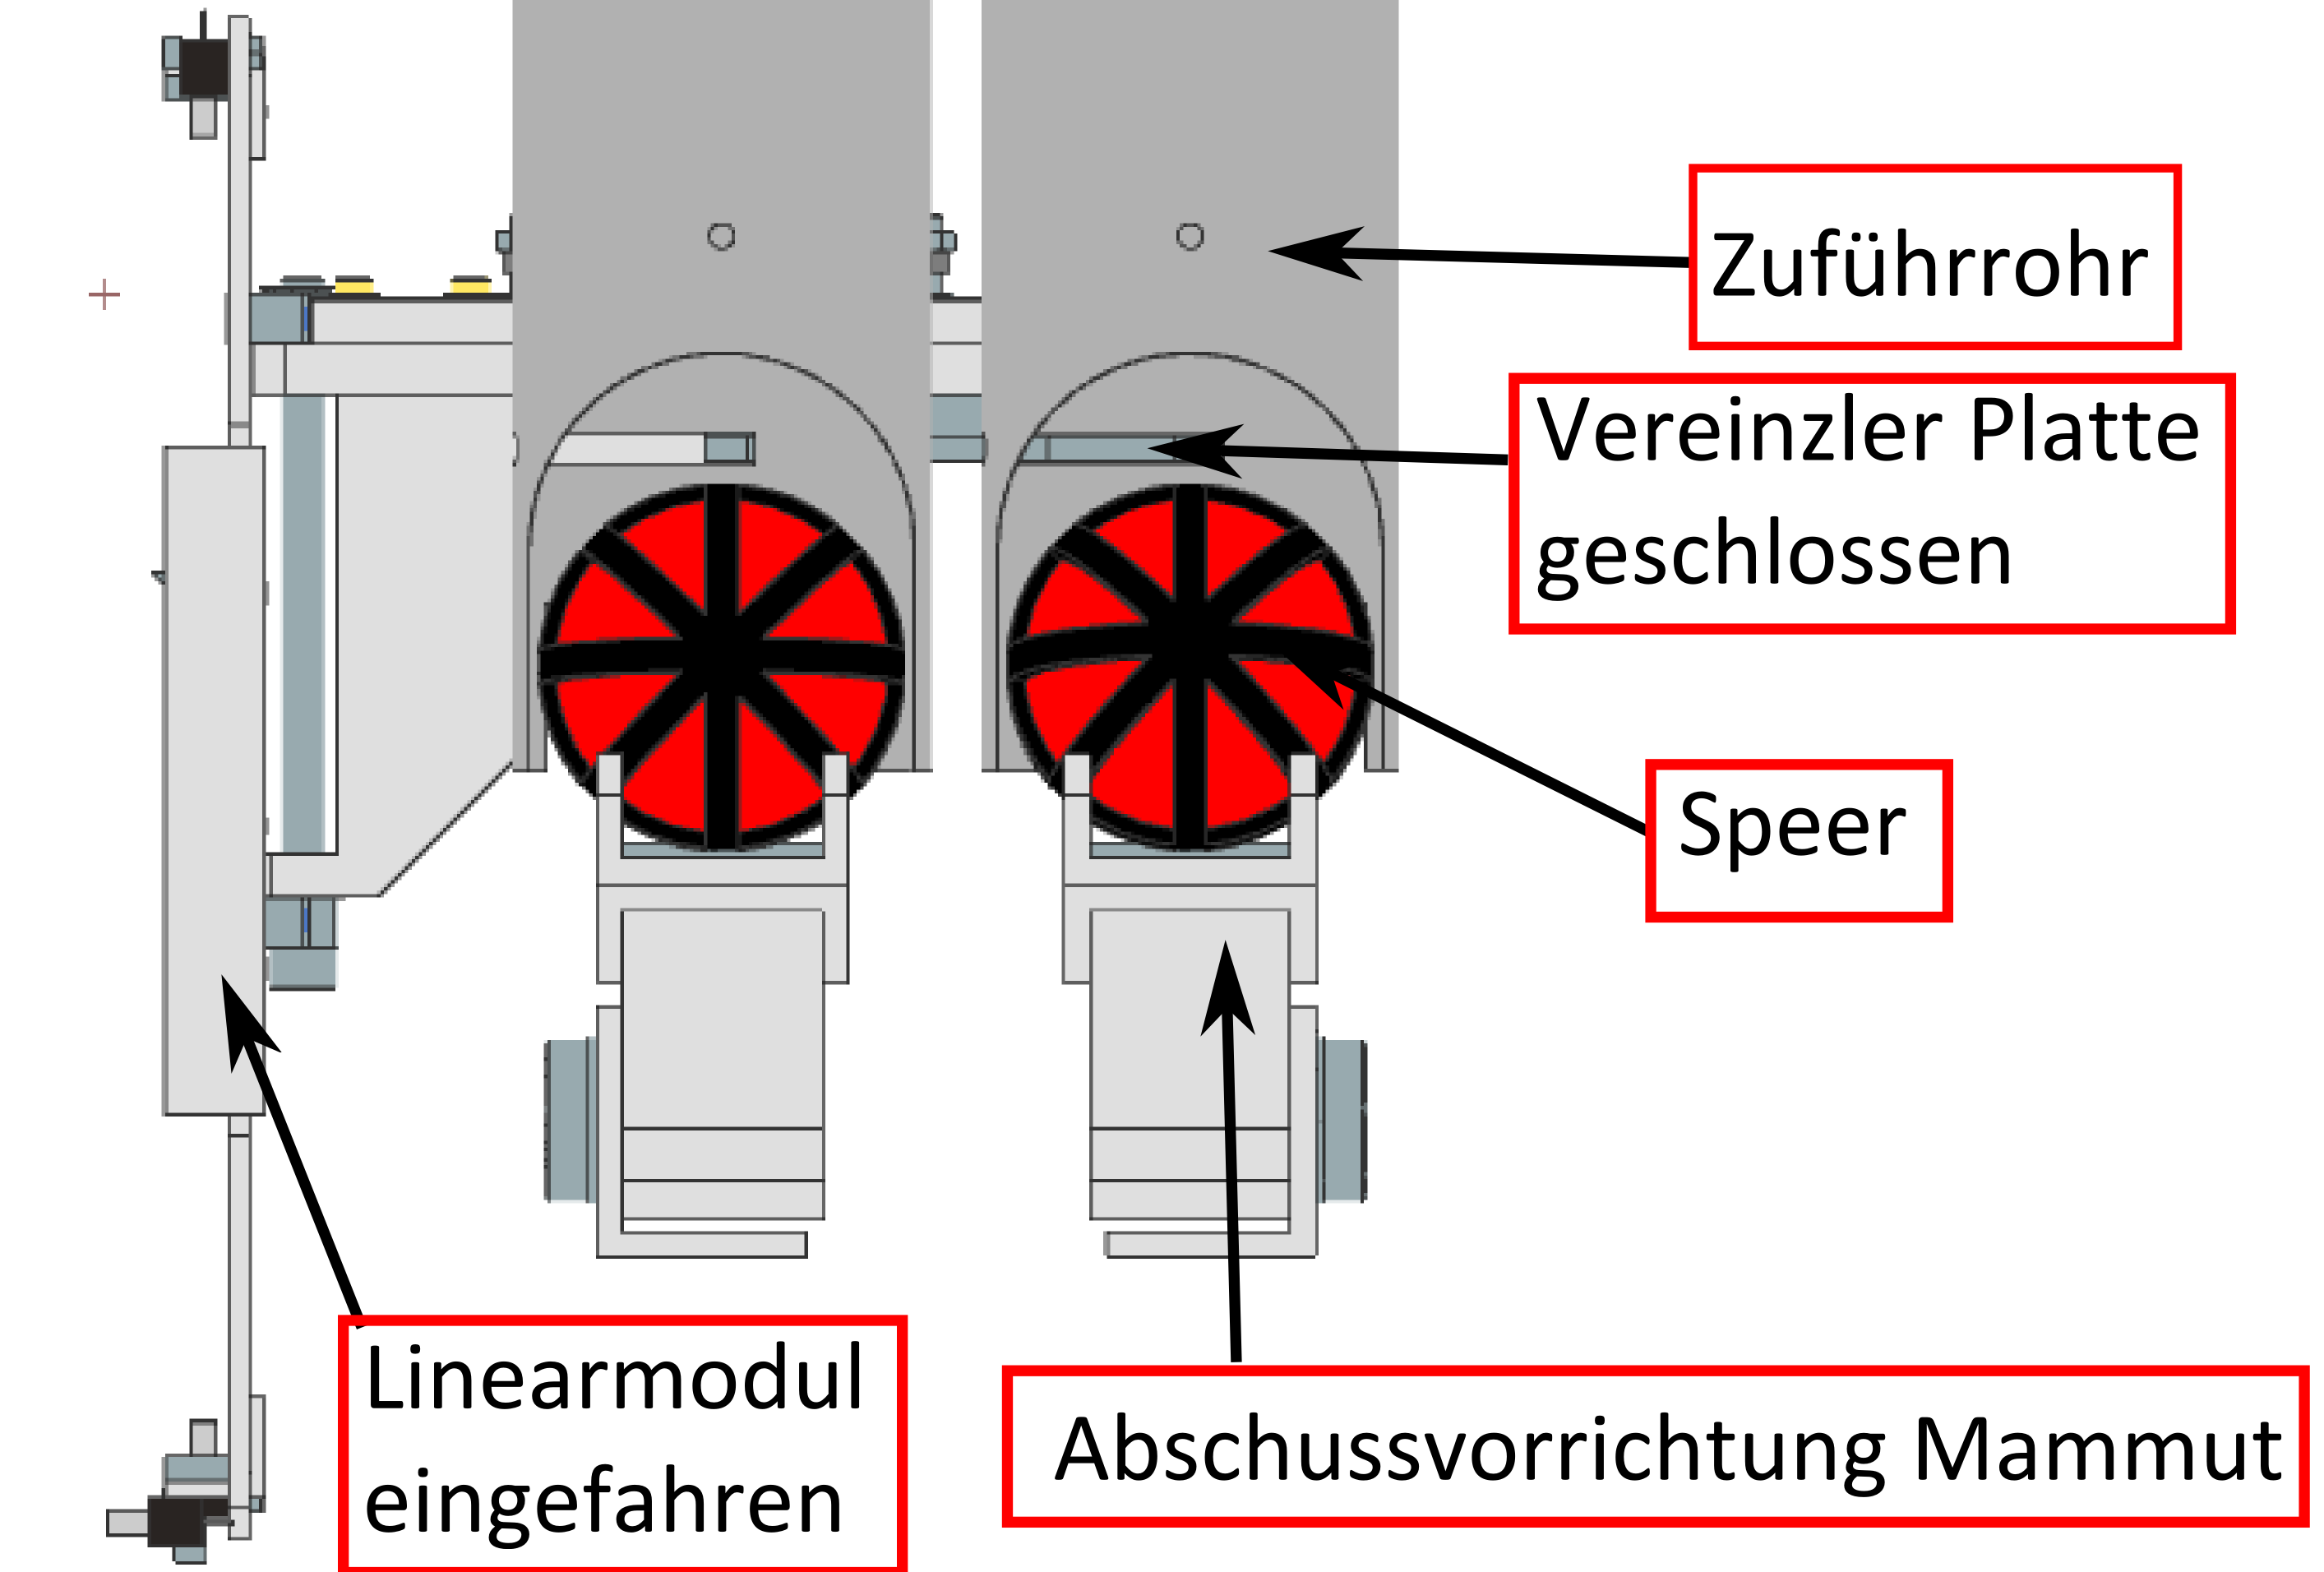
\includegraphics[height=5cm]{content/image/Mechanik_PA2/Aenderungen/Vereinzelung_Vorderansicht_geschlossen}  
						\caption{Geschlossen}
						\label{abb:vor_zu}          
					\end{subfigure}
					\begin{subfigure}[b]{0.49\textwidth}
						\centering
							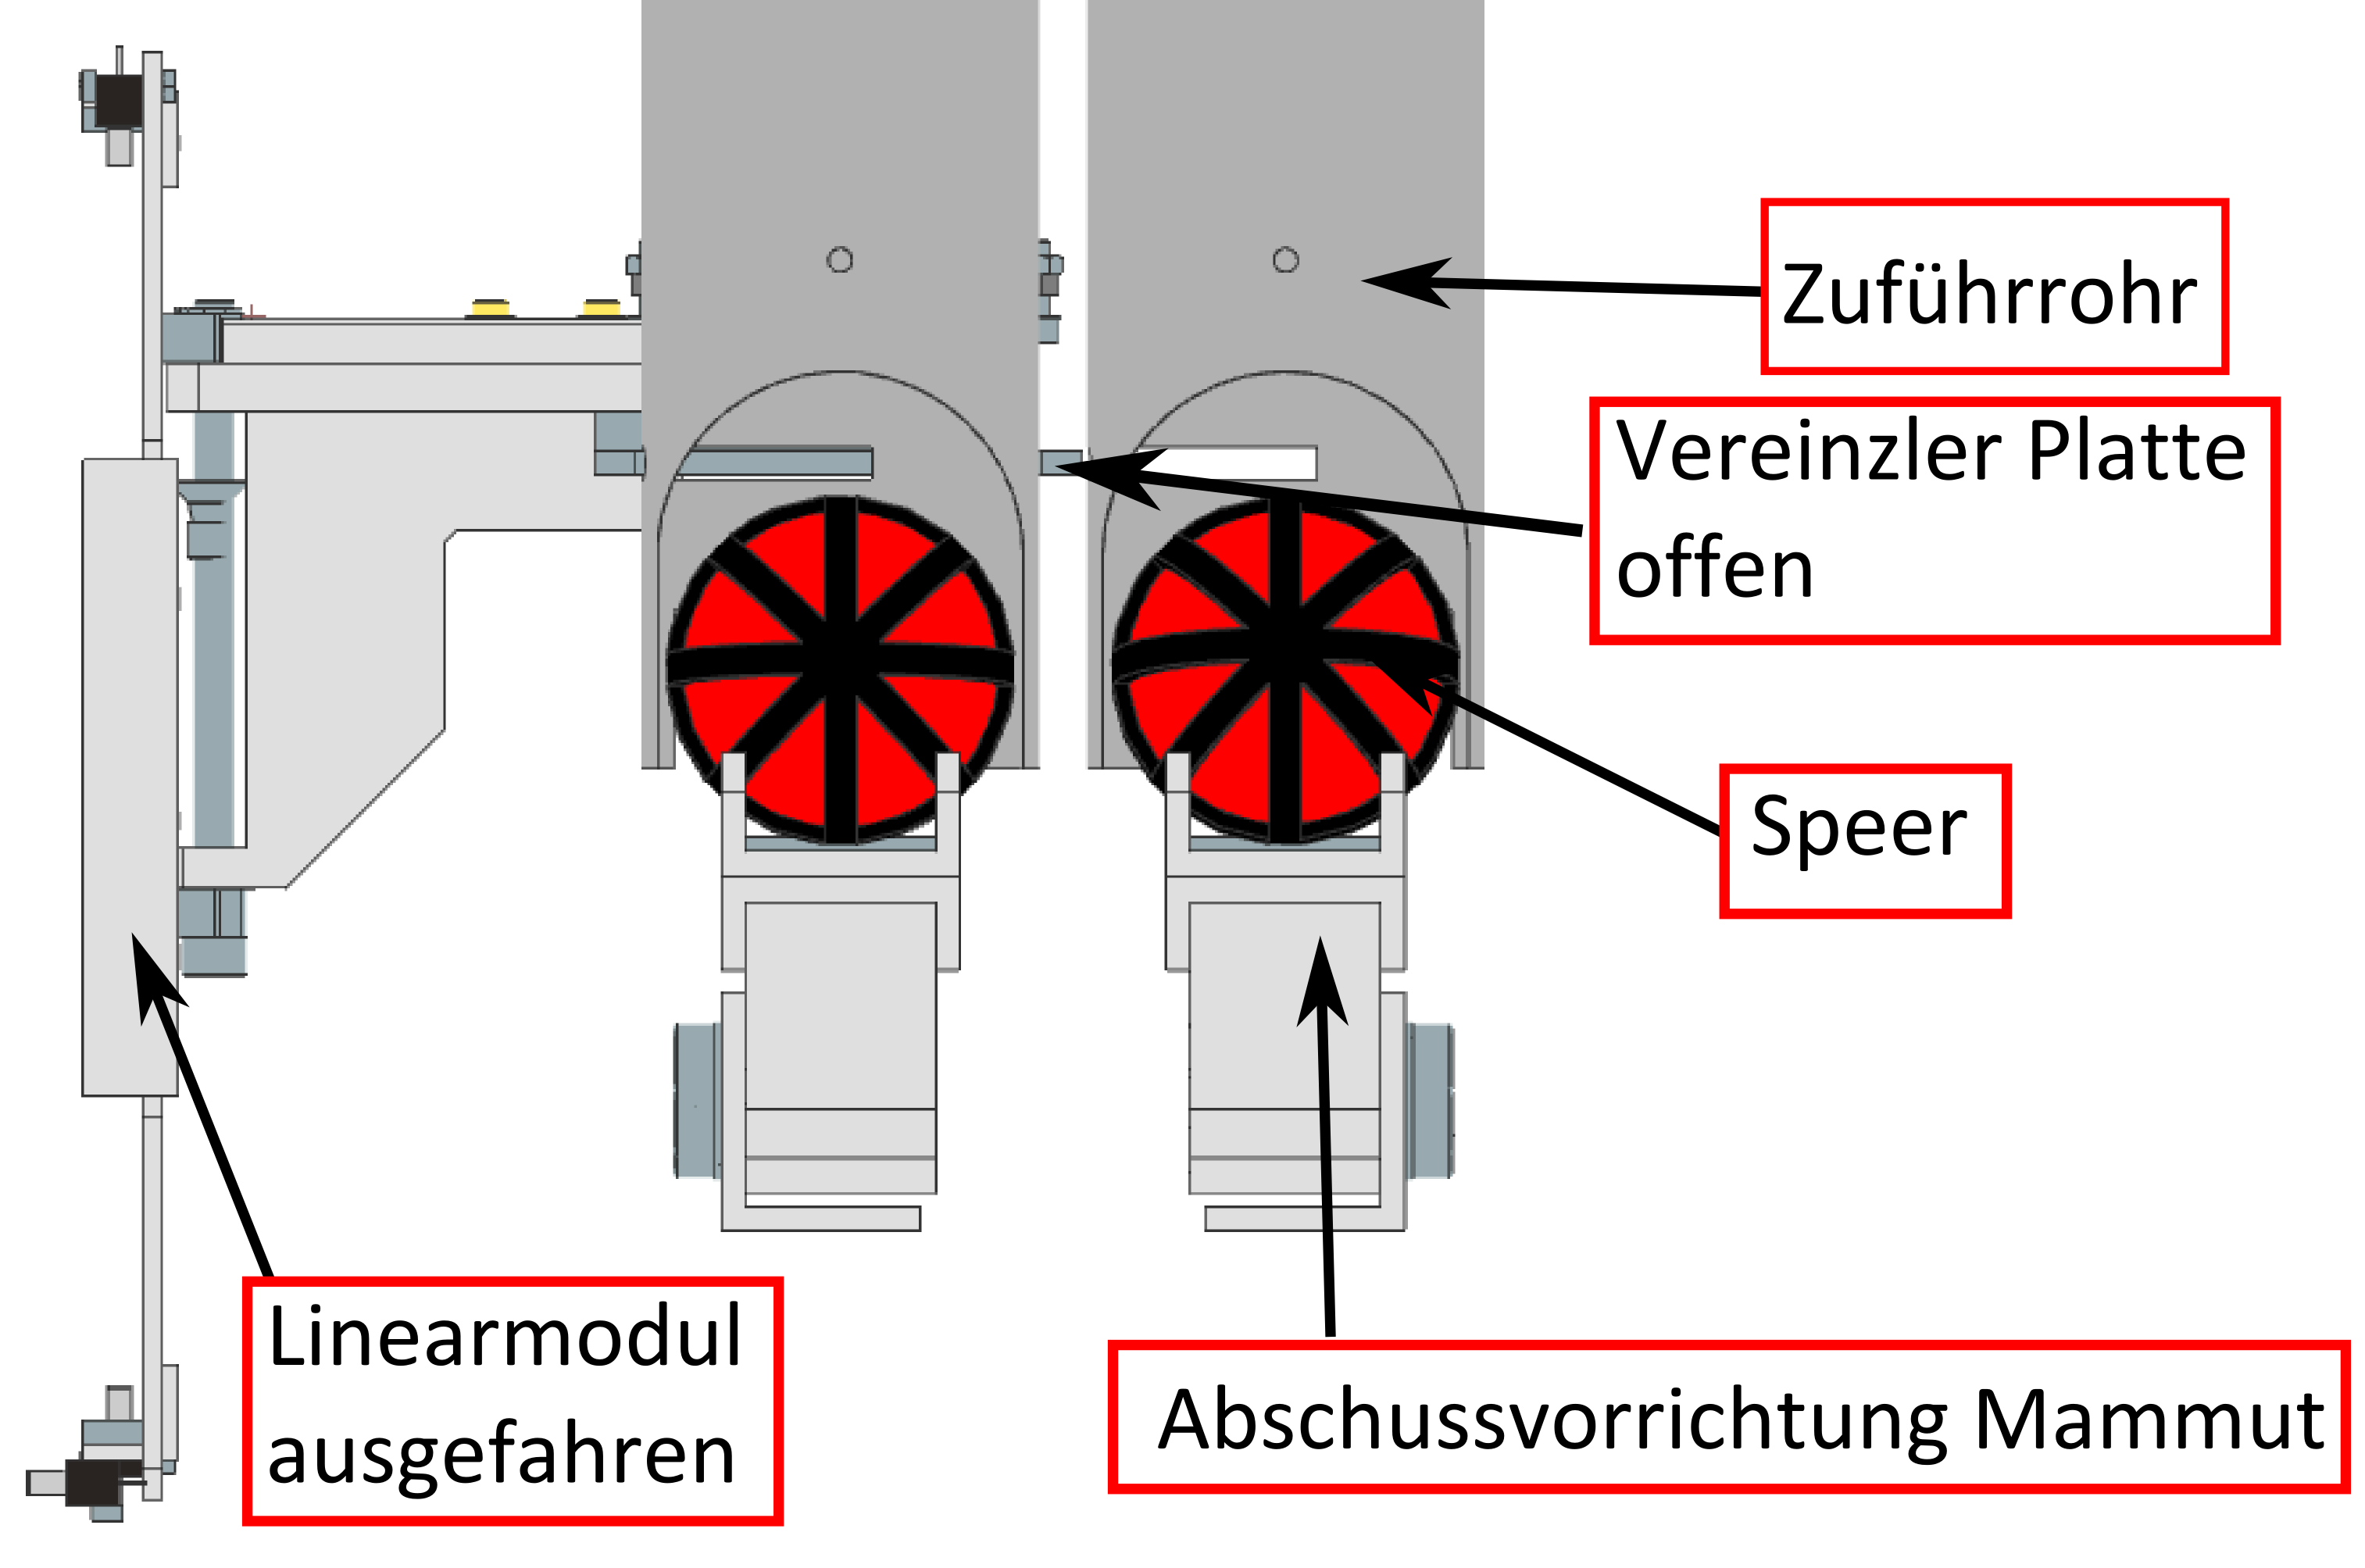
\includegraphics[height=5cm]{content/image/Mechanik_PA2/Aenderungen/Vereinzelung_Vorderansicht_offen}   
						\caption{Offen} 
						\label{abb:vor_offen}         
					\end{subfigure}
					\caption{Vereinzler vorderansicht}
					\label{abb:vor}
		    	\end{figure}
		    	%
				\begin{figure}[htbp] %htbp
					\centering
					\begin{subfigure}[b]{0.49\textwidth}
						\centering
						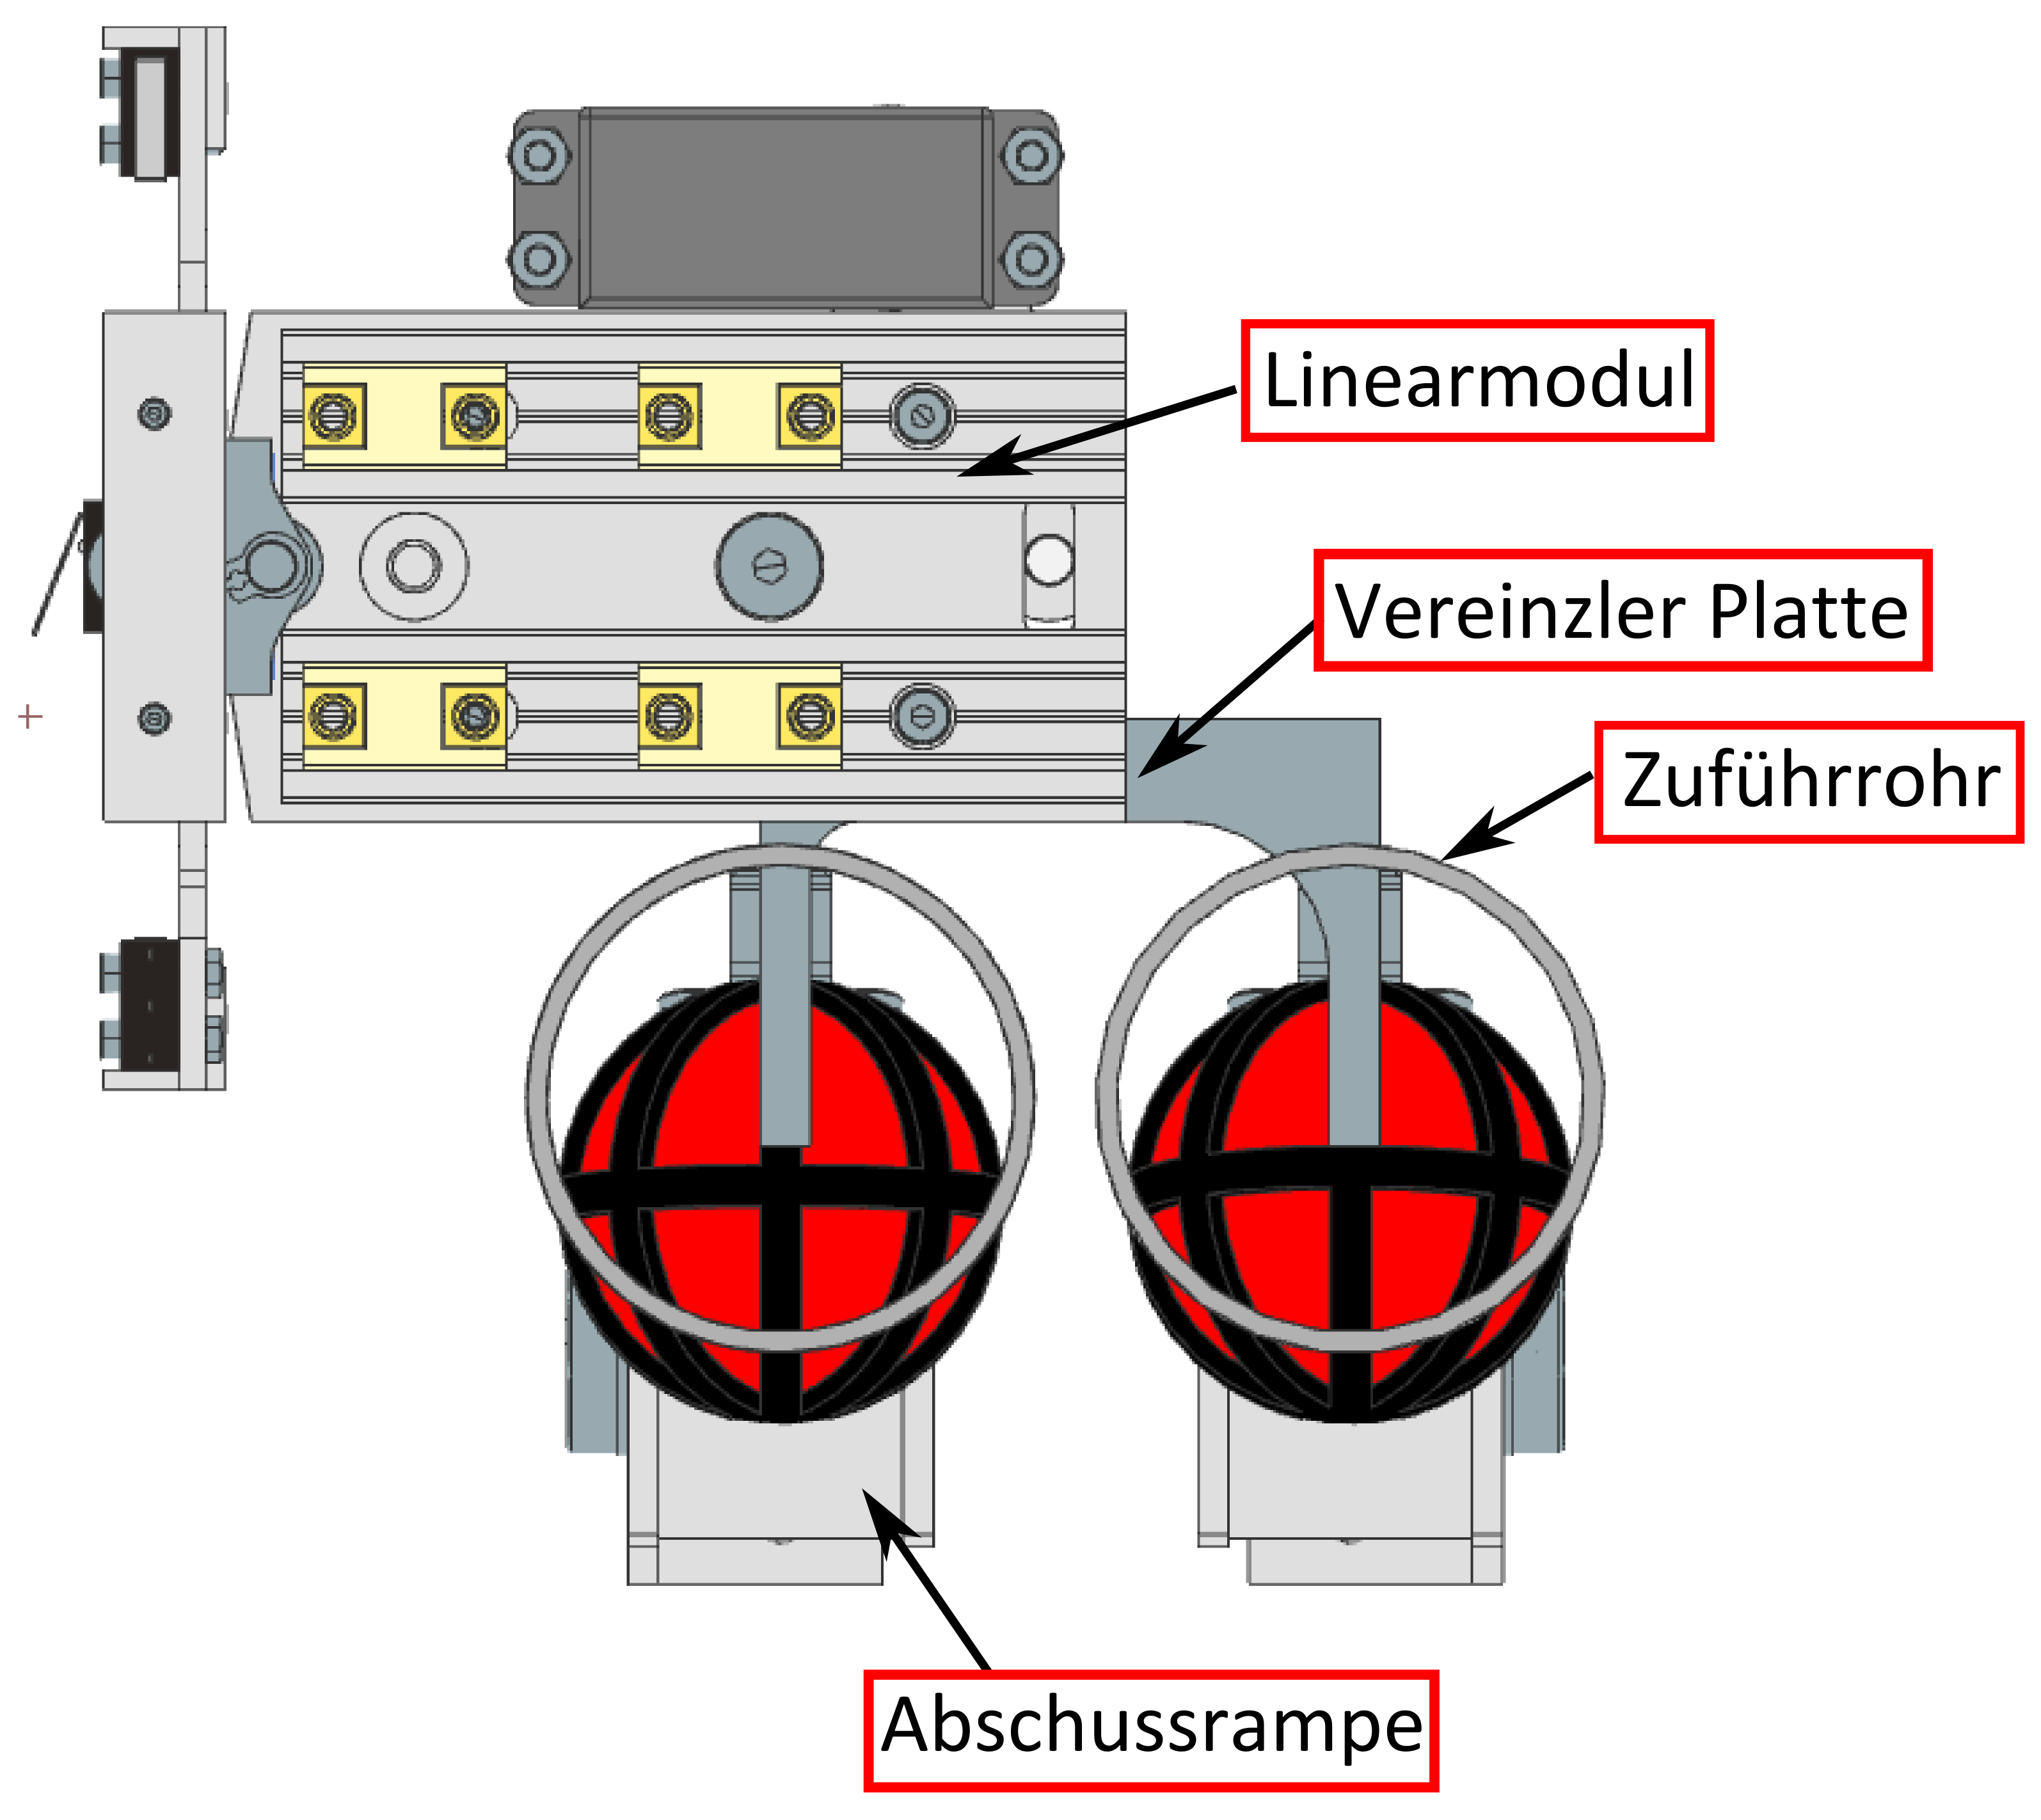
\includegraphics[height=6cm]{content/image/Mechanik_PA2/Aenderungen/Vereinzelung_Aufsicht_geschlossen}  
						\caption{Geschlossen}
						\label{abb:auf_zu1}          
					\end{subfigure}
					\begin{subfigure}[b]{0.49\textwidth}
						\centering
							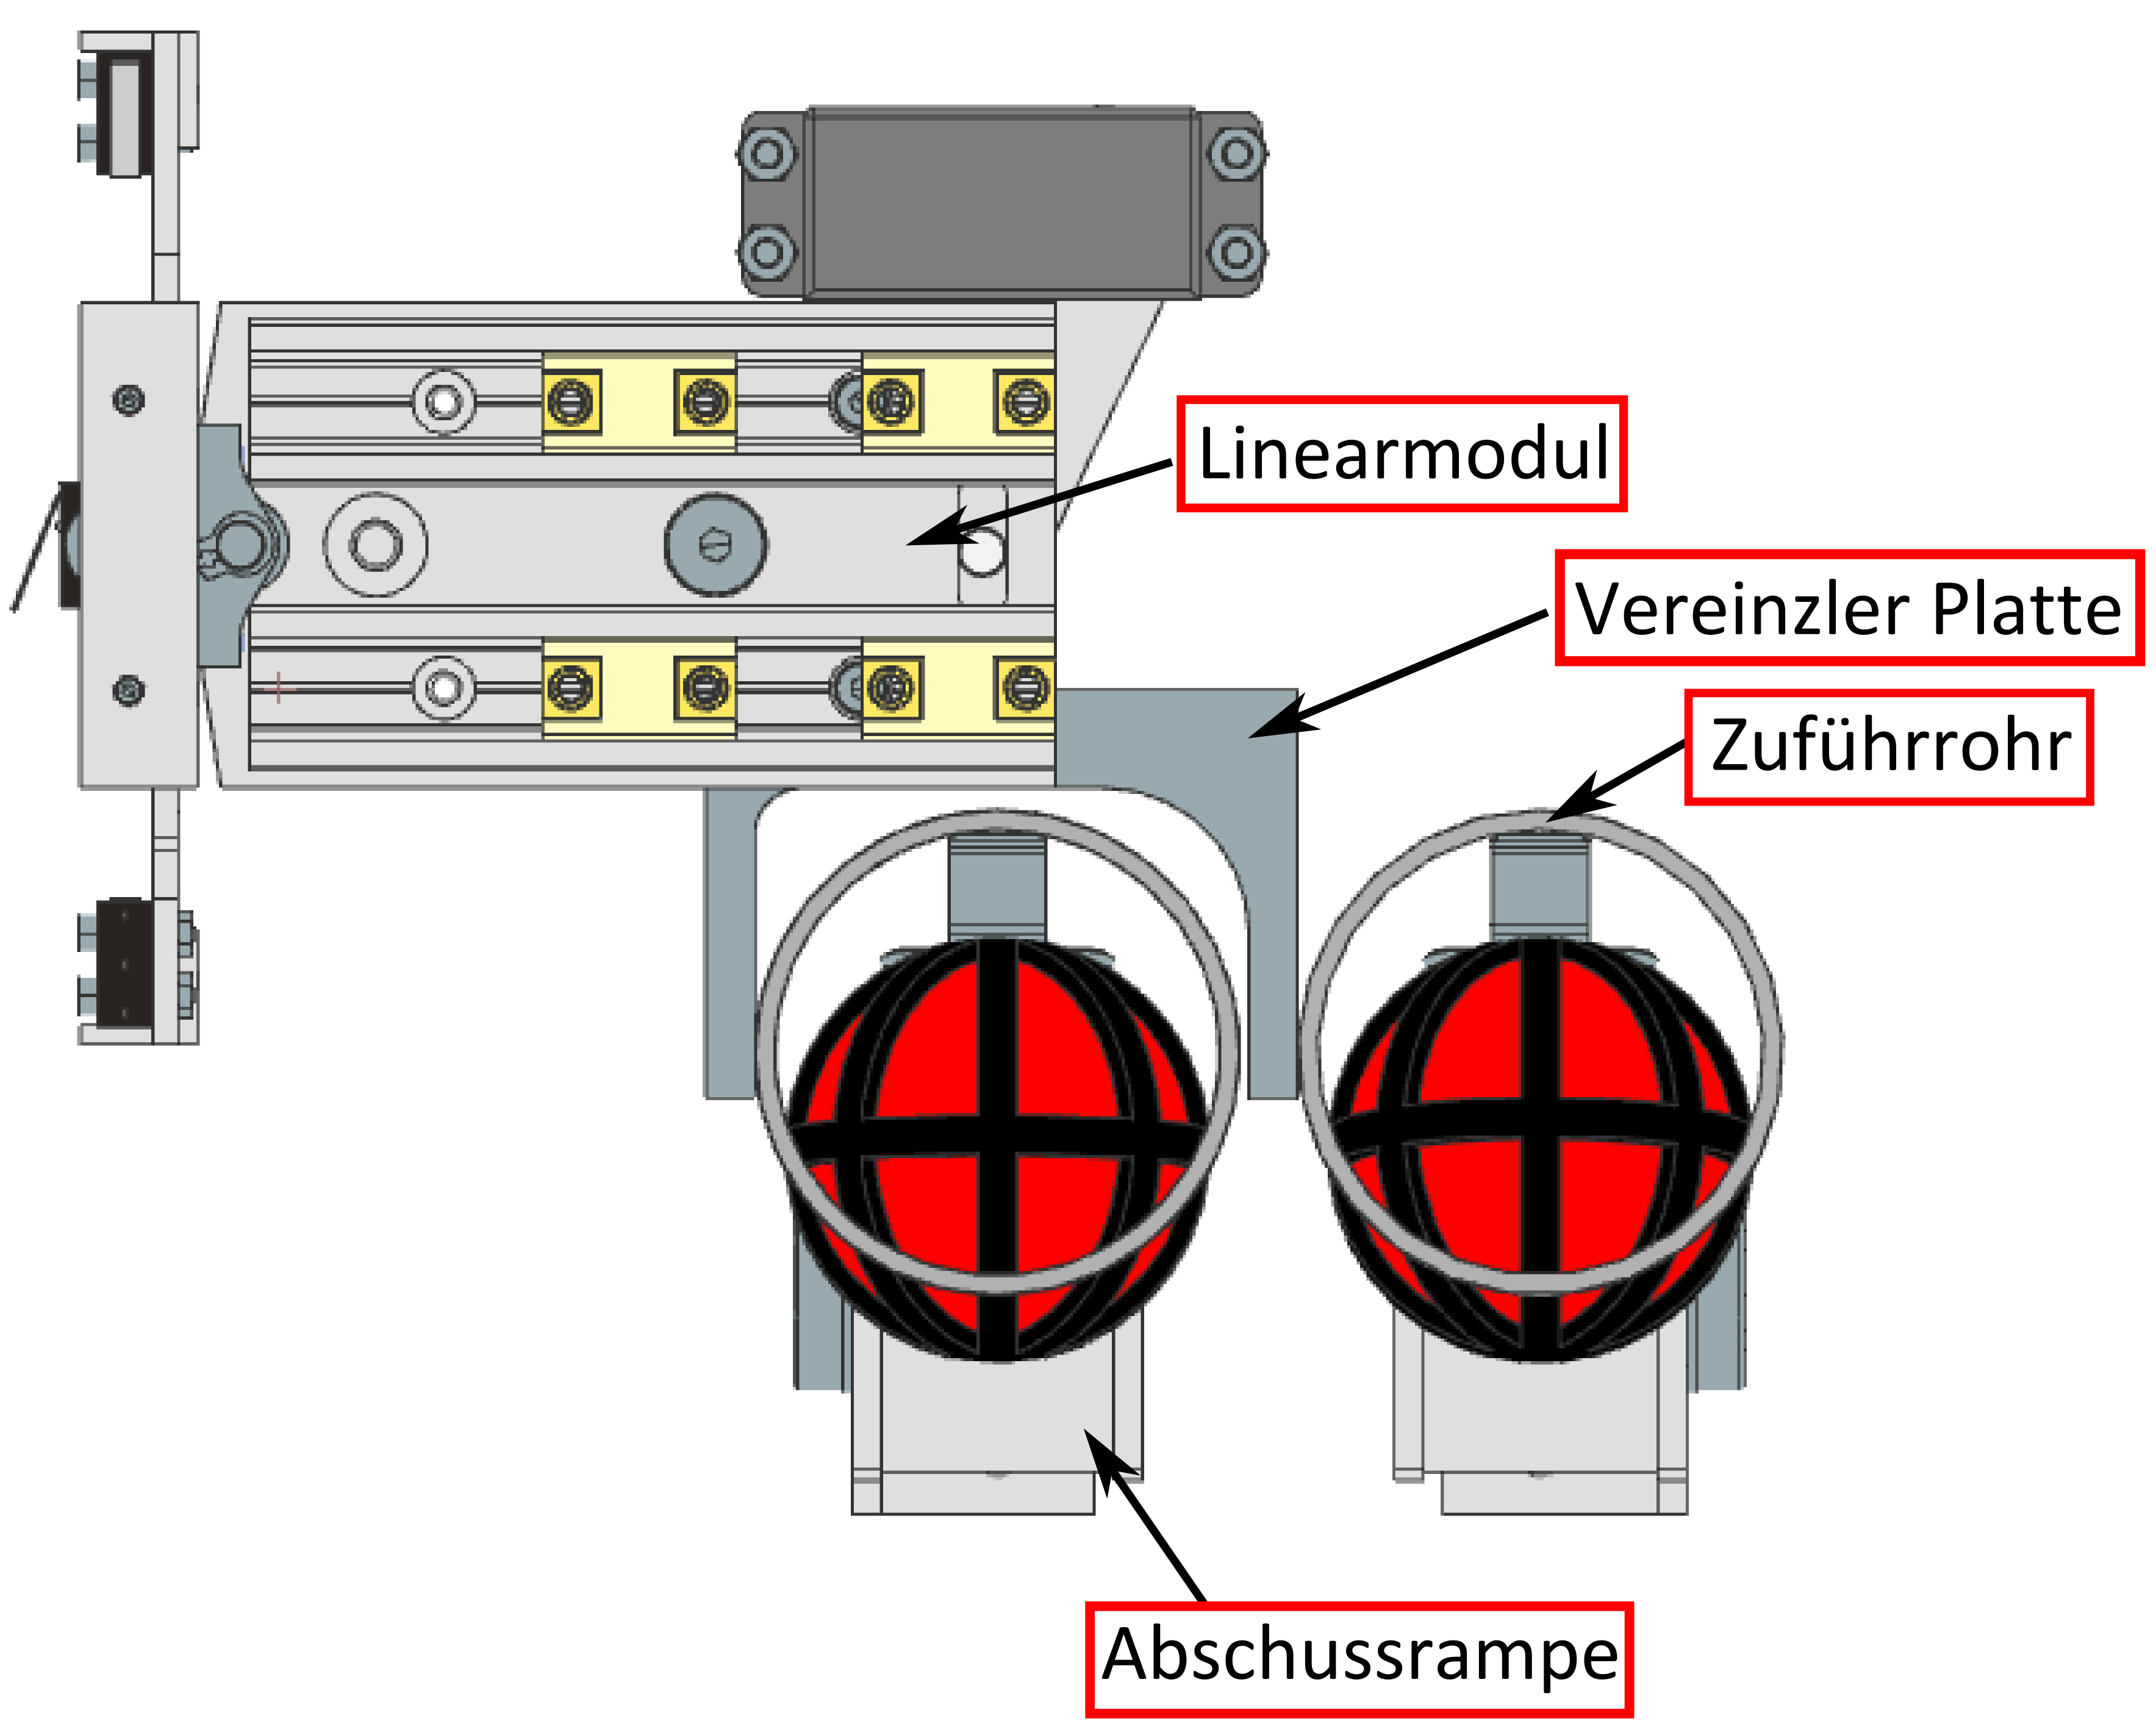
\includegraphics[height=6cm]{content/image/Mechanik_PA2/Aenderungen/Vereinzelung_Aufsicht_Offen}   
						\caption{Offen} 
						\label{abb:auf_offen1}         
					\end{subfigure}
					\caption{Vereinzler Aufsicht}
					\label{abb:auf}
		    	\end{figure}
		    	%
			%
			\newpage
			\paragraph{Zuf�hrrohre}
				Die Resultate aus der ersten Testreihe (siehe Anhang F) zeigten, dass die Zuf�hrrohre vorne einen zu grossen Ausschnitt haben. Denn beim Nachrutschen der Speere kam es dazu, dass die Speere ab der Abschussrampe fielen. Damit mehr seitliche F�hrung durch die Zuf�hrrohre generiert werden kann, wird eine Tasche gefr�st anstelle mittigen Auftrennens des Zuf�hrrohres. Weiter ist durch den, wie vorhin erw�hnt, gr�sseren Spannwinkel eine Kollision mit der Klinkenwelle und dem Zuf�hrrohr m�glich. Deshalb wurde der Ausschnitt f�r die Klinkenwelle und Blattfeder vergr�ssert. F�r die Vereinzelung sind zus�tzlich Nuten in die Zuf�hrrohre eingebracht (siehe Abbildung \ref{abb:rohr_nach}). Mit der Umstellung auf die Vereinzelung entf�llt der Ausschnitt f�r die Navigationseinheit, da die Rohrposition nicht mehr einstellbar sein muss. (siehe Abbildung \ref{abb:rohr_vor})
				%
				\vspace{-20pt}
				\image{content/image/Mechanik_PA2/Aenderungen/zufuehrrohr_alt}{scale=0.5}{htbp}[Zuf�hrrohr rechts vor Korrektur][abb:rohr_vor]
				\vspace{-30pt}
				%
				\image{content/image/Mechanik_PA2/Aenderungen/zufuehrrohr_neu}{scale=0.55}{htbp}[Zuf�hrrohr rechts nach Korrektur][abb:rohr_nach]
			%
			\paragraph{Steg Abschussrampe}
				Beim Spannen der Blattfeder verliert der Speer den Kontakt mit der Blattfeder. Dadurch rutschen die Speere auf der Abschussrampe leicht nach hinten. Damit die Position der B�lle w�hrend dem Spannen der Blattfeder konstant bleibt ist ein Steg in die Abschussrampe geklebt worden. Zus�tzlich soll der Steg die Blattfeder bremsen, so dass diese nur noch kurze Zeit �berschwingt. (siehe Abbildung \ref{abb:absch_mit_steg} Abschussrampe mit Steg) 
				%
				\image{content/image/Mechanik_PA2/Aenderungen/Steg}{scale=0.6}{htbp}[Abschussrampe mit Steg][abb:absch_mit_steg]
			%
		%
		\newpage
		\subsection{Anpassungen Fresko}\label{ss:anpassungen_fresko}	
			\paragraph{Servo}
				Das Servo ist neu definiert worden, dies aus dem Grund, weil das eingesetzte Servo ein Restposten war aus vorherigen Jahren und es im Betrieb nicht �berzeugt. Weiter kommt hinzu dass durch die Vereinzelung der Speere eine weitere Aufgabe von diesem Servoantrieb abh�ngig ist. Neu ist ein Servo von Hitec HS 7985MG im Einsatz. (siehe Anhang E Datenbl�tter)
			%
		%
		\subsection{Anpassungen Antrieb}\label{ss:anpassungen_antrieb}	
			\paragraph{Distanzscheibe}
				Drehgeber Das Befestigungsgewinde am Drehgeber ist nicht bis an die Schulter durchg�ngig. Dadurch konnte der Drehgeber nicht an die Schulter gezogen werden. Mit einer Distanzscheibe von 1mm Dicke konnte der dies behoben werden (siehe Abbildung \ref{abb:distanzscheibe_drehgeber}).
				%
				\image{content/image/Mechanik_PA2/Aenderungen/Distanzscheibe_Drehgeber}{scale=0.5}{htbp}[Distanzscheibe Drehgeber][abb:distanzscheibe_drehgeber]
			%
			\newpage
			\paragraph{Distanzscheibe Rad}
				Das Rad streifte das Rad des Drehgebers. Damit kein Kontakt zwischen den beiden R�dern mehr passiert, wurde eine Distanzscheibe auf die Sechkantwelle montiert. (siehe Abbildung \ref{abb:distanzscheibe_auf_sechskantwelle})
				%
				\image{content/image/Mechanik_PA2/Aenderungen/Distanzscheibe_Sechstkant}{scale=0.5}{htbp}[Distanzscheibe auf Sechstkantwelle][abb:distanzscheibe_auf_sechskantwelle]
			%
			\paragraph{Radkappen}
				Mit der �nderung der Distanzscheibe und den Abmassen der zugekauften R�der stellte sich heraus, dass die Sechstkantwelle zu lang ist und �ber das Rad hinausragte (siehe Abbildung 19 Rad montiert ohne Radkappe). Damit das Rad Befestigt werden kann ist eine Radkappe konstruiert worden. (siehe Abbildung \ref{abb:rad} und Abbildung \ref{abb:radkappe})
				%
				\begin{figure}[htbp] %htbp
					\centering
					\begin{subfigure}[b]{0.49\textwidth}
						\centering
						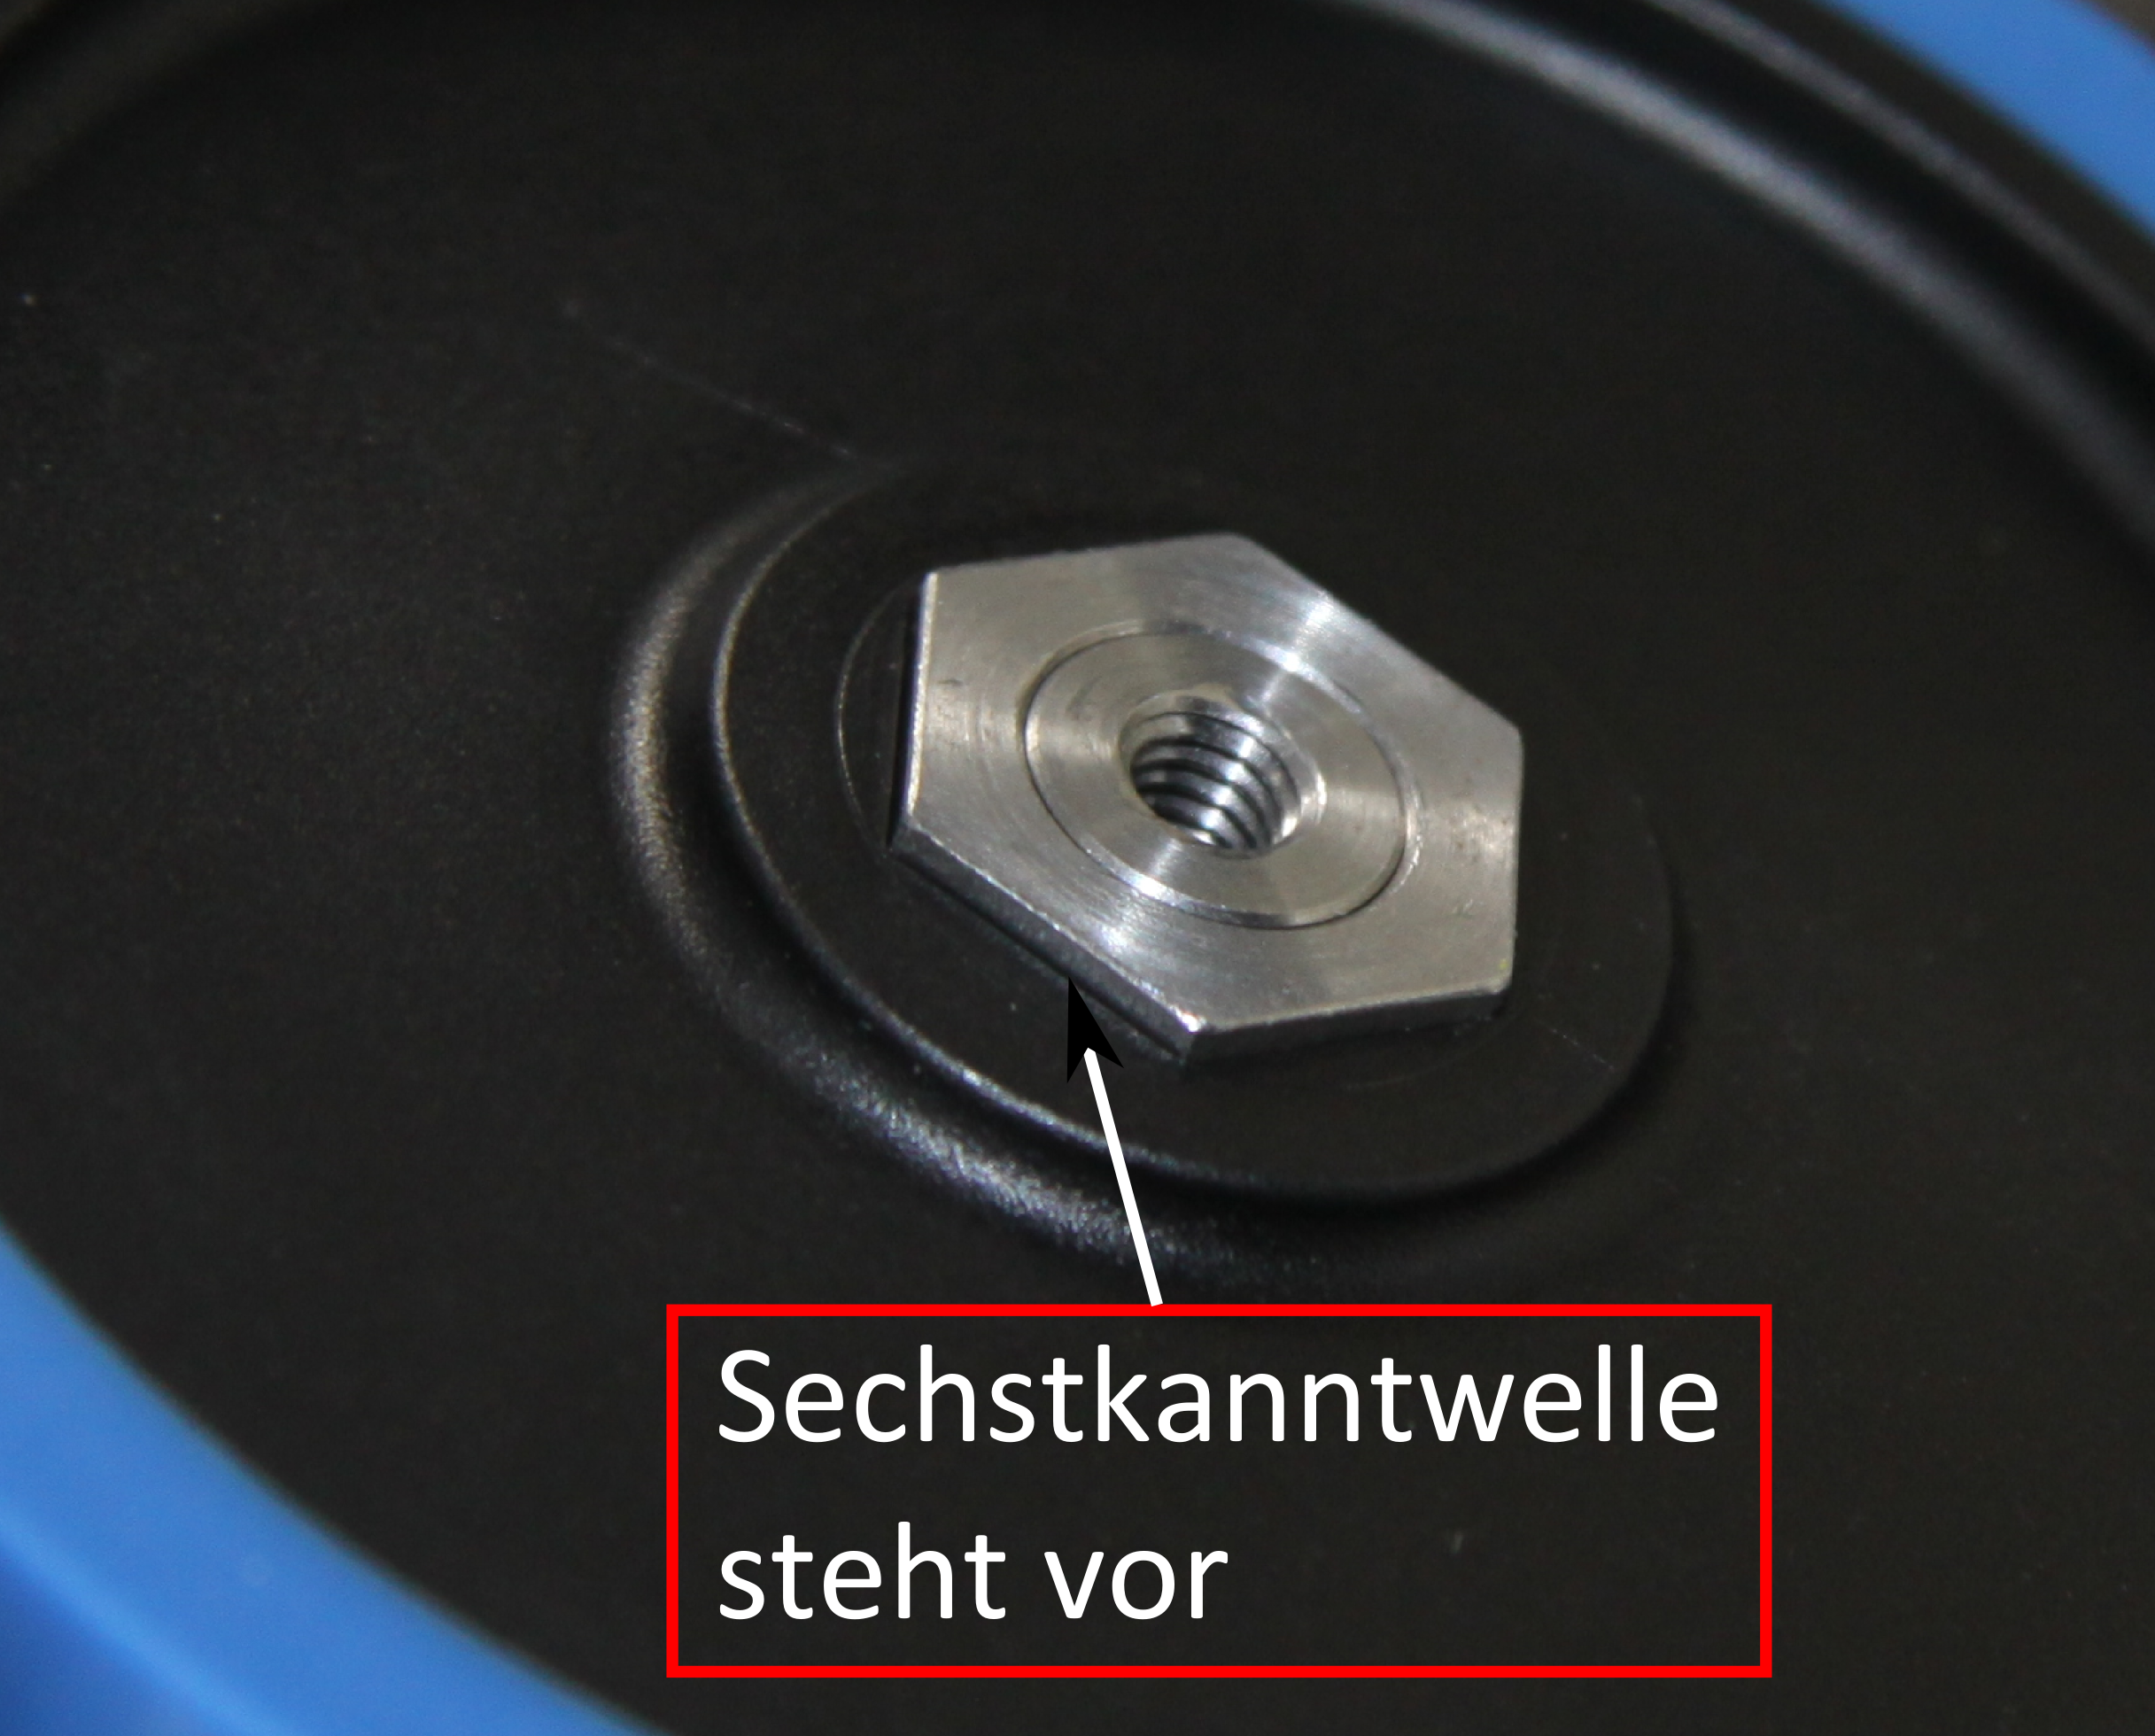
\includegraphics[height=5cm]{content/image/Mechanik_PA2/Aenderungen/Rad_montiert_ohne_Radkappe}  
						\caption{Ohne Radkappe}
						\label{abb:radkappe_ohne}          
					\end{subfigure}
					\begin{subfigure}[b]{0.49\textwidth}
						\centering
							\includegraphics[height=5cm]{content/image/Mechanik_PA2/Aenderungen/Rad_montiert_mit_Radkappe}   
						\caption{Mit Radkappe} 
						\label{abb:radkappe_mit}         
					\end{subfigure}
					\caption{Rad montiert}
					\label{abb:rad}
		    	\end{figure}
		    	%
				%\image{content/image/Mechanik_PA2/Aenderungen/40120_Radkappe}{scale=1}{htbp}[Radkappe][abb:radkappe]
		
%
%Kapitel 5: Hardware
%%%%%%%%%%%%%%%%%%%%%%%%%%%%%%%%%%%%%%%%%%%%%%%%%%%%%%%%%%%%%%%%%%%%%%%%%%%%%%%
% Titel:   Hardware
% Autor:   haldj3
% Datum:   17.04.2014
% Version: 0.0.1
%%%%%%%%%%%%%%%%%%%%%%%%%%%%%%%%%%%%%%%%%%%%%%%%%%%%%%%%%%%%%%%%%%%%%%%%%%%%%%%
%
%:::Change-Log:::
% Versionierung erfolgt auf folgende Gegebenheiten: -1. Release Versionen
%                                                   -2. Neue Kapitel
%                                                   -3. Fehlerkorrekturen
%
% 0.0.1       Erstellung der Datei
%%%%%%%%%%%%%%%%%%%%%%%%%%%%%%%%%%%%%%%%%%%%%%%%%%%%%%%%%%%%%%%%%%%%%%%%%%%%%%%    
\chapter{Hardware}\label{ch:hardware_pa2}
	%
	%Bedieneinheit
	\section{Bedieneinheit}\label{s:hw_bedieneinheit}
		Da vor jeder Spielrunde w�hrend dem Eurobot-Turnier die Teamzuteilung (Rot o. Gelb) alternieren kann und sonstige Initialisierung, wie z.B. die Quantit�t der gegnerischen Roboter, eingestellt werden m�ssen, ben�tigen unsere Roboter eine Bedienoberfl�che.\\
		Das Kernteam hat daher beschlossen ein einfaches Bedienpanel mit einem kleinem LCD Display (2x16) und mehreren Tastern zu entwickeln (Abbildung \ref{pic:bedienpanel}). Diese Aufgabe fiel dem Kernteammitglied Jascha zu und stellt damit der Hauptbestandteil seiner Projektarbeit 2 (PA2) dar.
		\par
		\image{content/image/Bedienpanel/Bedienpanel}{scale=0.8}{htbp}[Bedienpanel Eurobot 2014][pic:bedienpanel]
		%
		Im Folgenden sollen die einzelnen Bestandteile und Entwicklungsschritte dieser Arbeit n�her erl�utert werden. Die Dokumentation der dazugeh�rigen Software ist im Kapitel \ref{s:sw_bedieneinheit} zu finden.
		%
		\subsection{Schnittstellen}\label{ss:schnittstellen}
			Damit das Bedienpanel keinen eigenen Mikrocontroller braucht und da das RoboBoard noch eine unbenutzte SPI-Schnittstelle hat, soll die Steuerung auf dem Controller des RoboBoards realisiert werden. Unser Bedienpanel braucht folge dessen eine SPI-Schnittstelle. Es handelt sich dabei um eine 10-Pin-Buchse (X1) mit folgender Pin-Bezeichnung (gleich wie beim RoboBoard) und -Verwendung:
	 		\begin{table}[H]
		    	\centering
		    	\caption{10-Pin-Buchse X1}
		    	\begin{tabular}{|c|c|p{11cm}|} 
		    		\hline
		    		\rowcolor{bfhblue}
		    		\textcolor{white}{Pin} & \textcolor{white}{Bezeichnung} & \textcolor{white}{Beschreibung der Verwendung}\\
					\hline
					1 & 5V & Speisungs-Pin\\
					\hline
					2 & SPI\_SCK & System clock der SPI-�bertragung\\
					\hline
					3 & SPI\_MISO & Wird f�r die Steuerung des Displays (RS-Pin) benutzt, da kein direkter Datenaustausch vom Display (Slave) zum RoboBoard (Master) ben�tigt wird\\
					\hline
					4 & SPI\_MOSI & Unidirektionale Daten�bertragung vom RoboBoard (Master) zum Display (Slave)\\
					\hline
					5 & SPI\_CS1 & Chip select-Pin\\
					\hline
					6 & SPI\_CS2 & Wird als weiteres I/O f�r den Taster 1 benutzt\\
					\hline
					7 & SPI\_IO1 & Wird als I/O f�r den Taster 2 benutzt\\
					\hline
					8 & SPI\_IO2 & Wird als I/O f�r den Taster 3 benutzt\\
					\hline
					9 & SPI\_TIM & Wird ebenfalls als I/O benutzt und auf eine 3-Pin-Buchse mit einer Schutzschaltung gef�hrt\\
					\hline
					10 & GND & Speisungs-Pin\\
					\hline
				\end{tabular}
			\label{tab:10-pin-buchse}
			\end{table}
			 %	
			Des weiteren wurde vom Speisungsteam gew�nscht, eine Zustands-LED (D1) vom LIPO-W�chter auf den Print des Bedienpanels anzubringen.
			\par
			Damit ergibt sich folgendes Blockdiagramm mit s�mtlichen Schnittstellen (Abbildung \ref{pic:blockdiagramm schnittstellen}):
			\par
			\image{content/image/Bedienpanel/Schnittstellen}{scale=1}{htbp}[Blockdiagramm Schnittstellen][pic:blockdiagramm schnittstellen]
			%
		\subsection{Displayauswahl}\label{ss:displayaswahl}
			F�r die Auswahl eines passenden Displays wurde eine Anforderungsliste erstellt:
	        \begin{itemize}
				\item Alphanumerisch
				\item 2x16 (2 Zeilen mit je 16 darstellbare Zeichen)
				\item Blau mit weisser Schrift (nicht rot oder gelb, damit keine Teamfarbe)
				\item SPI
				\item Speisung: 5 V oder sogar 3.3 V kompatibel, damit keine Treiber n�tig
				\item Hintergrundbeleuchtung
	        \end{itemize}
			Daraus ergaben sich vier LCD Displays, die diese Anforderungen erf�llen. Die Datenbl�tter dieser, befinden sich im elektronischen Anhang.\\
			Um die Auswahl zu begrenzen wurden sekund�re Anforderungen definiert:
	        \begin{itemize}
				\item Schriftgr�sse > 5 mm
				\item Nicht l�nger als 80 mm (aus Platzgr�nden in den Robotern)
	        \end{itemize}
	        %
			Dies hatte zur Folge, dass die Auswahl auf folgende zwei Displays begrenzt wurde:
			%
			\subsubsection{NHD-0216K3Z}\label{sss:NHD}
				Der Vorteil dieses Displays (Abbildung \ref{pic:nhd}) ist das ausf�hrliche Datenblatt und die vielen SW-Vorlagen. Der Nachteil ist die Dicke des Displays mit dem dazugeh�rigen Print und die Montageart auf dem eigentlichen Print der Bedieneinheit.
		 		\par
		 		\image{content/image/Bedienpanel/nhd_display}{scale=0.5}{htbp}[NHD (80x36x13.3mm)][pic:nhd]
		 		%
			\subsubsection{EA DOGM162}\label{sss:DOGM}
				Der Vorteil diese Displays (Abbildung \ref{pic:dogm}) ist die geringe Dicke, da es direkt auf den Print gel�tet werden kann und die allgemein kompakte Ausf�hrung mit dessen ungeachtet markt�blicher Schriftgr�sse von 5.57 mm. Des weiteren ist es 3.3 V kompatibel. Ein Nachteil ist das sp�rliche Datenblatt. Dieses Problem kann jedoch mit der Hilfe von diversen Erfahrungskommentaren im Internet entgegengewirkt werden.
		 		\par
		 		\image{content/image/Bedienpanel/dogm_display}{scale=1}{htbp}[DOGM (55x31x3.6mm)][pic:dogm]
		 		%
				=> Die Wahl fiel schlussendlich auf den EA DOGM162. Der entscheidende Vorteil gegen�ber dem New Heaven Display (NHD-0216K3Z) ist die 3.3 V Kompatibilit�t, was den Zeitaufwand in der Entwicklung und die Bauteilkosten reduziert.
				%
		\subsection{Schema}\label{ss:schema}
			%
			\subsubsection{Speisung}
				Da das Display 3.3 V kompatibel ist und somit direkt mit dem Mikrocontroller des RoboBoards verbunden werden kann, ist es naheliegend die vorhandenen 5 V herunter zu wandeln. Umgesetzt wurde dies mit dem MCP1700, welcher ein 5 V zu 3.3 V low dropout (LDO) Spannungsregler ist.\par
				Da das Display mit der Hintergrundbeleuchtung einen maximal Strom von 60.2 mA ben�tigt, betr�gt die maximale Verlustleistung:\par
				$ P_{v_{max}} = \Delta U \cdot I_{max} = (5 V - 3.3 V) \cdot 60.2 mA = \underline{102.34 mW} $\par
				Mit einem $ R_{JA} $ von 52�C/W entspricht dies einer Temperaturerh�hung von 5.3 �C, was als problemlos betrachtet wird. 
				%
			\subsubsection{Display und Hintergrundbeleuchtung}			
				Das Datenblatt des DOGM162 enth�lt verschiedene Applikationsbeispiele die je nach Kommunikationsart und Speisespannung variieren. Verwendet wurde folge dessen dasjenige mit 3.3 V und SPI (Abbildung \ref{pic:applikationsbeispiel}).
		 		\par
		 		\image{content/image/Bedienpanel/Display_Schema}{scale=0.5}{htbp}[Applikationsbeispiel][pic:applikationsbeispiel]
		 		%
				Die Hintergrundbeleuchtung ist monochrom und hat zwei separate LED-Pfade, welche parallel oder in Serie geschaltet werden k�nnen. Diese ben�tigen externe Widerst�nde zur Strombegrenzung. Die Vorw�rtspannung der weissen LED's betr�gt 3.2 V (parallel geschaltet) und der maximale Strom 30 mA pro Pfad. Mit der Betriebsspannung von 3.3 V ergibt dies �ber dem Widerstand einen Spannungsabfall von 0.1 V.\par
				$ R_{min} = \frac{U}{I_{max}} = \frac{0.1 V}{30 mA} = 3.33 \Omega $  -> Wahl: $ \underline{3.9 \Omega} $ (E12-Reihe) 
		 		\par
		 		($P_{v_{R}} = \frac{U^{2}}{R} = \frac{(0.1 V)^{2}}{3.9 \Omega} = 2.56 mW$)
		 		\par
		 		Das Display und die Hintergrundbeleuchtung (Abbildung \ref{pic:display mit hintergrundbeleuchtung}) wurden im Schema zusammen gezeichnet, damit sie der Realit�t entsprechend, im gleichen Bauteil vereint sind.
		 		\par
		 		\image{content/image/Bedienpanel/Display_mit_Hintergrundbeleuchtung}{scale=0.5}{htbp}[Display mit Hintergrundbeleuchtung][pic:display mit hintergrundbeleuchtung]
		 		%
			\subsubsection{Sensor/Aktor-Eingang mit Schutzschaltung}
				Der Aufbau dieser Schaltung entspricht derjenigen vom RoboBoard. Sie wurde umgesetzt, da ein I/O-Pin der Schnittstelle zum RoboBoard nicht ben�tigt wurde, m�glicherweise aber ein weiterer Sensor oder Aktor angeschlossen werden m�chte.
				Die Kondensatoren C6, C7 und C8 sind St�tzkondensatoren. Der Widerstand R3 dient als Schutz im Fehlerfall. Der Pull-Up-Widerstand im Mikrocontroller des RoboBoards betr�gt gem�ss Datenblatt 40 kOhm. Mit dem gew�hlten Widerstand von 120 Ohm ergibt dies eine Verlustleistung ($ P_{R_{max}} $) von:\par
				$ I_{max} = \frac{U}{R_{PU} + R_{3}} = \frac{3.3 V}{40 k\Omega + 120 \Omega} = 82.3 \mu A $ \par
				$ P_{R_{max}} = I_{max}^{2} \cdot R_{3} = (82.3 \mu A)2 \cdot 120 \Omega = \underline{0.8 \mu W } $ und beim Pull-Up: \underline{271 $ \mu W $}
	 			%
	 			\image{content/image/Bedienpanel/Sensor_Schema}{scale=0.5}{htbp}[Sensor/Aktor-Eingang][pic:sensor/aktor-eingang]
	 			%
			\subsubsection{Taster}
				Die drei Taster wurden als Active-Low angeschlossen, um die internen Pull-Ups des Mikrocontrollers des RoboBoards zu nutzen.
		 		\par
		 		\image{content/image/Bedienpanel/Taster}{scale=0.7}{htbp}[Taster][pic:taster]
		 		%
				Zum Entprellen der Taster wurden je 10 nF Kondensatoren dazu geschaltet. Dieser Wert gilt als Standard und kann folgendermassen hergeleitet werden:\\
				Die Prellzeit ist stark vom Schaltertyp abh�ngig. Sie wird jedoch auf ca. 10 ms gesch�tzt [Quelle: mikrocontroller.net/articles/Entprellung]. In dieser Zeit darf der Mikrocontroller folge dessen noch nicht auf einen Wert von kleiner 1 V (Logisches 0) fallen. Damit dies eingehalten wird, soll sich die Spannung in dieser Zeit lediglich um etwa 1 V �ndern. Der Input Leakage Current des Mikrocontrollers des RoboBoards (STM32F4) ist max. 1 uA.\\
				Es gilt: \par 
				$  I = C \cdot \frac{dU}{dt} $ -> $ C = I \cdot \frac{dt}{dU} = 1 \mu A \cdot \frac{10 ms}{1 V} = \underline{10 nF} $ \par
				Sollte dennoch ein st�rendes Prellen festgestellt werden, k�nnte ein Entprellen auch in der SW realisiert werden.
				%
		\subsection{Layout}\label{ss:layout}
			Das Layout des Bedienpanel ist einseitig (Bottom-Layer) mit einem GND-Plane und Leiterbahnbreiten von mindestens 20 mil. Bis auf den selbst erstellten Footprint des Displays sind s�mtliche Footprints aus der Standardbibliothek. Da das Bedienpanel im Roboter nach Aussen zug�nglich sein muss, m�ssen s�mtliche Buchsen abgewinkelt sein. Dies musste im Layout vor allem bei der 10-Pin-Buchse ber�cksichtigt werden, da aus Zeitgr�nden kein passender Footprint erstellt wurde. Es wurde ausserdem darauf geachtet, dass die Taster einen gen�gend grossen Abstand zu den h�heren Bauteilen und je einen Abstand von 1 cm zueinander haben, um die Bedienung zu erleichtern.\\
			Die Prints f�r beide Roboter k�nnen intern (mit der Fr�se) innerhalb eines Tages hergestellt werden.
			%
		\subsection{Inbetriebnahme}\label{ss:inbetriebnahme}
			Das Testen der Funktionalit�t der Hardware wurde parallel zum Best�cken durchgef�hrt. Dabei wurde vorg�ngig ein Inbetriebnahme-Protokoll definiert, welches im elektronischen Anhang zu finden ist. Dabei wurden prim�r die Speisungen und nebeneinander liegende Leitungen auf Kurzschl�sse �berpr�ft.\\
			Die gemessenen Werte entsprachen den Erwartungen.
			%
	%
	%CAN-Adapter
	\section{CAN-Adapter}\label{s:can-adapter}
		Ebenfalls von Jascha wurden vier CAN-Adapter (Abbildung \ref{pic:can_adapter} \& \ref{pic:can_adapter_layout}) angefertigt, die das Debuggen der CAN-Kommunikation erleichtern sollen. Sie enthalten zwei 10-Pin-Buchsen (X1 \& X2), eine D-Sub-Buchse (J1) und eine 3-Pin-Stiftleiste (X3) f�r Messabgriffe. Ausserdem kann wahlweise ein 150 Ohm Abschlusswiderstand (R1) mit einem Jumper (X4) dazugeschaltet werden.
		\par
		\image{content/image/Bedienpanel/CAN_Adapter}{scale=0.6}{htbp}[CAN-Adapter Schema][pic:can_adapter]
		%
		\par
		\image{content/image/Bedienpanel/CAN_Adapter_Layout}{scale=0.6}{htbp}[CAN-Adapter Layout][pic:can_adapter_layout]
		%
%
%Kapitel 6: Software
%%%%%%%%%%%%%%%%%%%%%%%%%%%%%%%%%%%%%%%%%%%%%%%%%%%%%%%%%%%%%%%%%%%%%%%%%%%%%%%
% Titel:   Software
% Autor:   gross10, mert1
% Datum:   22.09.2013
% Version: 0.0.1
%%%%%%%%%%%%%%%%%%%%%%%%%%%%%%%%%%%%%%%%%%%%%%%%%%%%%%%%%%%%%%%%%%%%%%%%%%%%%%%
%
%:::Change-Log:::
% Versionierung erfolgt auf folgende Gegebenheiten: -1. Release Versionen
%                                                   -2. Neue Kapitel
%                                                   -3. Fehlerkorrekturen
%
% 0.0.1       Erstellung der Datei
%%%%%%%%%%%%%%%%%%%%%%%%%%%%%%%%%%%%%%%%%%%%%%%%%%%%%%%%%%%%%%%%%%%%%%%%%%%%%%%    
\chapter{Software}\label{ch:software_pa2}
	W�hrend der \gls{ac:pa2} wurden die Software-Designs der \gls{ac:pa1} implementiert und bei Bedarf erg�ntzt. Es ist anzumerken, dass die entsprechenden Kapitel in der Dokumentation der \gls{ac:pa1} nicht aktualsiert wurden und deshalb veraltete Fakten beinhalten k�nnen.
	%
	%
	%System
	\section{System}\label{s:system}
		Das komplette System gliedert sich mehrere Komponente. Folgend wird detailiert auf einzelnen Aspekte eingegangen. Dabei wird Top $\rightarrow$ Buttom vorgegangen und nur der kleine Roboter betrachtet.
		%
		%
		\subsection{Roboter}
			F�r den Betrieb des Roboters werden diverse Aktoren und Sensoren eingesetzt, zu sehen im Kontextdiagramm \cref{pic:context}. 
			%
			\image{content/image/14_context}{scale=1}{htbp}[Kontextdiagramm][pic:context]
			%
			Alle diese Komponenten erf�llen eine spezifische Aufgabe:
			%
			\begin{itemize}
				\item Eing�nge
				\begin{description}
					\item[Odometrie links/rechts]
						Mit Hilfe der Odometrie ist eine relative Positionsbestimmung m�glich.
					%
					\item[Gyro]
						F�r eine absolute Winkelbestimmung muss ein Gyro eingesetzt werden.
					%
					\item[Ultraschall Navigation]
						Ein auf Ultraschall basierendes Positionierungssytem verschaft uns eine absolute Position w�hrend eines Matchs.
					%
					\item[Funk Navigation]
						F�r den Informationsaustasch zwischen den einzelnen Robotern wird eine Funkverbindung eingesetzt.
					%
					\item[Ultraschall Naherkennung]
						Um im nahen Umfeld des Roboters Gegest�nde (auch Gegener) genau zu erkenne wird ein einfacher Ultraschallsensor verbaut. Er liefert ab einer bestimmten Distanz\footnote{aktuell 20cm} genau Abstandsinformationen.
					%
					\item[Infrarot Naherkennung]
						F�r das einfache Erkennen von Hindernissen kommen zus�tzlich zum Ultraschallsensor noch Infrarotschalter zum Einsatz.
					%
					\item[Taster Fresko 1, 2 \& Wand]
						Um verifiziern zu k�nnen ob ein Fresko anklebt oder die Wand erreicht wurde, werden drei einfache Hubtaster eingesetzt.
					%
					\item[Taster Schl�ssel]
						Das Reglement schreibt vor, dass die Roboter mit dem Herausziehen einer Schnur gestartet werden m�ssen. In unserem Fall wird mit Hilfe der Schnur ein Schl�ssel aus seiner Verankerung verschoben, die wiederum einen Taster akiviert.
					%
					\item[Taster Notstopp]
						Ebenfalls vorgeschrieben ist ein Notstopp-Schalter. Dieser unterbricht zum einen die Stromversorgung zu allen Aktoren und zum anderen wird das System in einen definierten Zustand gesetzt.
				\end{description}
				%
				\item Ausg�nge
				\begin{description}
					\item[Motor links/rechts]
						Sind zust�ndig f�r die forbewegung des Roboters.
					%
					\item[Servo Mammut]
						Bet�tigt den Mechnismus zum abfeuern der B�lle
					%
					\item[Servo Fresko]
						Klebt als Hauptaufgabe die Freskos an die Wand. Weiter �bernimmt es noch die Vereinzelung der B�lle.
					%
					\item[Display]
						Dient zum einstellen aktueller Spielparameter wie Teamfarbe\footnote{Weitere Erl�uterungen dazu sind im \cref{s:hw_bedieneinheit} zu finden}.
					%
					\item[LED]
						Sind f�r visuelle Kontrolle des aktuellen Systemzustands zust�ndig (Normalbetrieb/Error).
				\end{description}
			\end{itemize}
		%
		%
		\subsection{Systemknoten}\label{ss:systemknoten}
			Der Roboter besteht aus drei Teilsysteme, die alle miteinander �ber den Feldbus \gls{ac:can} kommunizieren (siehe \cref{pic:systemknoten}). Jeder dieser sogenannten Bus-Knoten wird von einem separaten Subteam entwickelt.
			%
			\begin{description}
				\item[Kernknoten, \acrfull{ac:kernteam}]
					Dem Kernknoten unterliegt die Steuerung und Kontrolle des gesamten Systems. Weiter �bernimmt er die Ansteuerung der spielaufgaberelevanten Aktoren und Sensoren. Es ist Aufgabe des \gls{ac:kernteam} f�r seine Funktionialt�t zu sorgen. In den folgenden Abschnitten \ref{ss:kernknoten} und \ref{ss:systemzustaende} wird daher n�her auf seinen Aufbau eingegangen.
				%
				\item[Antriebsknoten, \acrfull{ac:antriebsteam}]
					Die Aufgabe des Antriebsknoten ist es prim�r f�r die Fortbewegung des Roboters zu sorgen. Weiter wird in ihm ein Wegfindealgorithmus und ein Kalman-Filter f�r eine exaktere Positionsbestimmung implementiert.
				%
				\item[Naviagtionsknoten, \acrfull{ac:navigationsteam}]
					Der Naviagtionsknote verschafft dem System Informationen �ber die aktullen absolute Position des Systems. Ausserdem �bernimmt es die Kommunikation mit den �brigen Robotern auf dem Spielfeld und tauscht mit ihnen Positionsinformationen aus.
			\end{description}
			%
			\image{content/image/14_dfd_level_1}{scale=1}{htbp}[DFD Systemknoten][pic:systemknoten]
			%
		%
		%
		\subsection{Kernknoten}\label{ss:kernknoten}
			Wie im vorherigen \cref{ss:systemknoten} erw�hnt, muss der Kernknoten die Systemsteuerung �bernehmen und die L�sung der Spielaufgaben erm�glichen. Dazu werden mehrere Tasks f�r die einzelnen Aufgabengebiete erstellt, die miteinander wie in \cref{pic:kernknoten} ersichtlich Verbunden sind.
			%
			\begin{description}
				\item[\gls{ac:can} RX/TX Task]
					Die \gls{ac:can} RX und TX Tasks sind Bestandteil des \gls{ac:can}-Gatekeepers. Sie werden im Anhang H erl�utert.
				%
				\item[\gls{ac:elp} Task]
					Der \gls{ac:elp} Task nutzt die von \gls{g:rtos} gegebene Funktion der Software-Timer. Diese bieten die M�glichkeit der zyklischen Ausf�hrung, sowie der einfachen Steuerung durch entsprechende Funktionen (start/stopp Timer). Innerhalb des Timers wird ein zyklisches \gls{ac:os} ausgef�hrt, das auf Basis des Timer-Zyklus periodisch \gls{ac:elp}-Anfoderungen an den \gls{ac:can}-Gatekeeper sendet. Die einzelen Positionsanforderungen werden wie folgt aufgerufen:
					\begin{itemize}
						\item Navi Position Request: alle 400ms
						\item Kalman Position Request: alle 600ms
						\item Confederate Position Request: alle 600ms
						\item Enemy 1 Position Request: alle 800ms
						\item Enemy 2 Position Request: alle 800ms
					\end{itemize}
					Die Befehle sind dem Anhang H entnommen. Die Periodizit�t muss eventuell noch an die realen Gegegbenheiten angepasst werden.
				%
				\item[Default Task]
					F�r die einfache Visualisierung des \gls{g:rtos}-Zustandes wird der Default Task eingesetzt. Wenn das System ohne Einschr�nkungen l�uft, so wird dies �ber Lichtspiel angezeigt. Im Falle eines Stackoverflows oder �ndlichen Misszust�nden wird das Lichtspiel angehalten.
				%
				\item[Knoten Task]
					Im Knoten Task werden die einzelen Aufgaben-Knoten, falls vom System Task gew�nscht, der Spielstrategie (siehe dazu \cref{s:speilstrategie}) abgearbeitet. Dies beinhaltet die Steuerung von Aktoren unter Ber�cksichtigung von Sensorwerten. Weiter muss eine Kommunikation mit dem Rangfinder Task bestehen um m�gliche Hindernisse w�hrend der Ausf�hrung zu erkennen.
				%
				\item[Rangfinder Task]
					F�r die Auswertung der Naherkennung ist der Rangfinder Task zust�ndig. Als Informationsquelle dienen ihm die zwei Ultraschallsensoren (hinten/vorne) und vier Infrarotschalter. Die Kommunikation zum Knoten Task erfolgt einerseit mit Hilfe einer Semaphore und andererseits mit globalen Zustandsflags.
				%
				\item[System Task]
					Die Abl�ufe der kompletten Applikation werden mit Hilfe des System Task gesteuert. Weiter erm�glicht erauch Benutzerinteraktionen durch entsprechende Taster (Schl�ssel/Notstopp) und Anzeige. F�r detailierte Information zu den einzelnen Systemzust�nden empfielt sich das \cref{ss:systemzustaende}.
				%
				\item[Timer Task]
					Eine Spielrunde dauert immer 90 Sekunden (+ 5 Sekunden Funny Action) \cite[]{lit:eurobot}. Sollte diese Zeit nicht eingehalten werden, so hat dies Punktabz�ge zur Folge. Um diesen Fall zur vermeiden wird der Timer Task eingesetzt. Seine Aufgabe besteht darin die Spielzeit zu �berwachen und bei Ablauf den Roboter zu stoppen (sollte die nicht bereits der Fall sein).
			\end{description}
			%
			\image{content/image/14_dfd_level_2}{scale=1}{htbp}[DFD Kernknoten][pic:kernknoten]
			%
			\subsubsection{Task-Priorit�ten}
				\gls{g:rtos} bietet die M�glichkeit einzelnen Task eine bestimmte Priorit�t zu vergeben. Somit k�nnen wichtige Teilbereiche eines Systems bevorzugt behandelt werden. Im vorliegenden Konzept sind dies haupts�chlich die Tasks des \gls{ac:can}-Gatekeepers und der Naherkennung.\par 
				%
				Die Priorit�t jedes spezifischen Tasks ist in der \cref{tab:prioritaeten} aufgef�hrt. Je h�her die Zahl, dessto h�her ist auch die Priorit�t.
				%
				\begin{table}[htbp]
				    \centering
				    \begin{tabular}{|l|l|} 
				        \hline
				        \rowcolor{bfhblue}
				        \textcolor{white}{Task Name} & \textcolor{white}{Priorit�t} \\
				        \hline
				        CAN RX/TX & 6\\
				        \hline
				        Rangfinder & 5 \\
				        \hline
				        \gls{ac:elp} & 4\\
				        \hline
				        Timer & 4\\
				        \hline
				        System & 3\\
				        \hline
				        Knoten & 2\\
				        \hline
				        Default & 1\\
				        \hline
				    \end{tabular}
				    \caption{Task Priorit�ten}
				    \label{tab:prioritaeten}  
				\end{table}
		%
		%
		\subsection{Systemzust�nde}\label{ss:systemzustaende}
			Das System kann sich ingesamt in vier Zust�nden befinden, die wiederum Unterzust�nde beinhalten k�nnen.
			%
			\begin{description}
				\item[Initialisierung]
					Im ersten Zustand werden alle Komponenten initialisiert, die zuvor, vor dem Start des \gls{g:rtos} Task-Schedulers, noch nicht gestartet werden konnten. Dies betrifft auf dem Kern Knoten die Anzeige-Einheit, die auf Verz�gerungsfunktionen des \gls{ac:os} angewiesen ist. Weiter wird das komplette System hinsichtlich der Erreichbarkeit von �brigen Feldbus-Knoten �berpr�ft. Sollte eine Teilkomponente nicht auf eine entsprechende Anfragen auf dem \gls{ac:can}-Bus antworten, so ist das System nicht funktionsf�hig und er Zustand wechselt zu Error.
				%
				\item[Setup]
				 	Im Setup werden Match betreffende Einstellungen vorgenommen. Dies beinhaltet die Parameter Teamfarbe, Anzahl Gegener/Verb�ndeter, Durchmesser der Gegner, sowie der gew�nschte Startknoten\footnote{F�r m�gliche Knoten-Identit�ten sei auf den \cref{s:speilstrategie} ab Seite \cpageref{s:speilstrategie} und insbesonders auf die \cref{abb:node_id} verwiesen.}. F�r die Men�-Navigation stehen drei Taster bereit, mit denen Schritt f�r Schritt die Einstellungen vorgenommen werden k�nnen (Ringmen�-Struktur). Ist die Parametriesierung abgeschlossen, so kann mit Hilfe des Schl�sselschalters der Roboter gestartet werden. 
				%
				\item[Run]
					Nachdem Abschluss der Konfiguration startet ein neuer Match. Die Kontrolle �ber die  einzelnen Teilaufgaben hat dabei der Run Zustand. Er �bernimmt strategische Entscheide und �bergibt dem Knoten Task entsprechende Information zum erf�llen einer Spielaufgabe. Die dabei angewandte Struktur ist im \cref{ss:match} erl�utert.
				%
				\item[Error]
					Sollte der Roboter nicht funktionsf�hig sein (z.B. keine Feldbus-Kommunikation), so befindet sich das System im Error Zustand. Dieser Zustand kann nicht verlassen werden und zwingt so den Bediener den aufgetretene Fehler genau zu analysieren. 
			\end{description}
			%
			\begin{figure}[htbp]
				\centering
				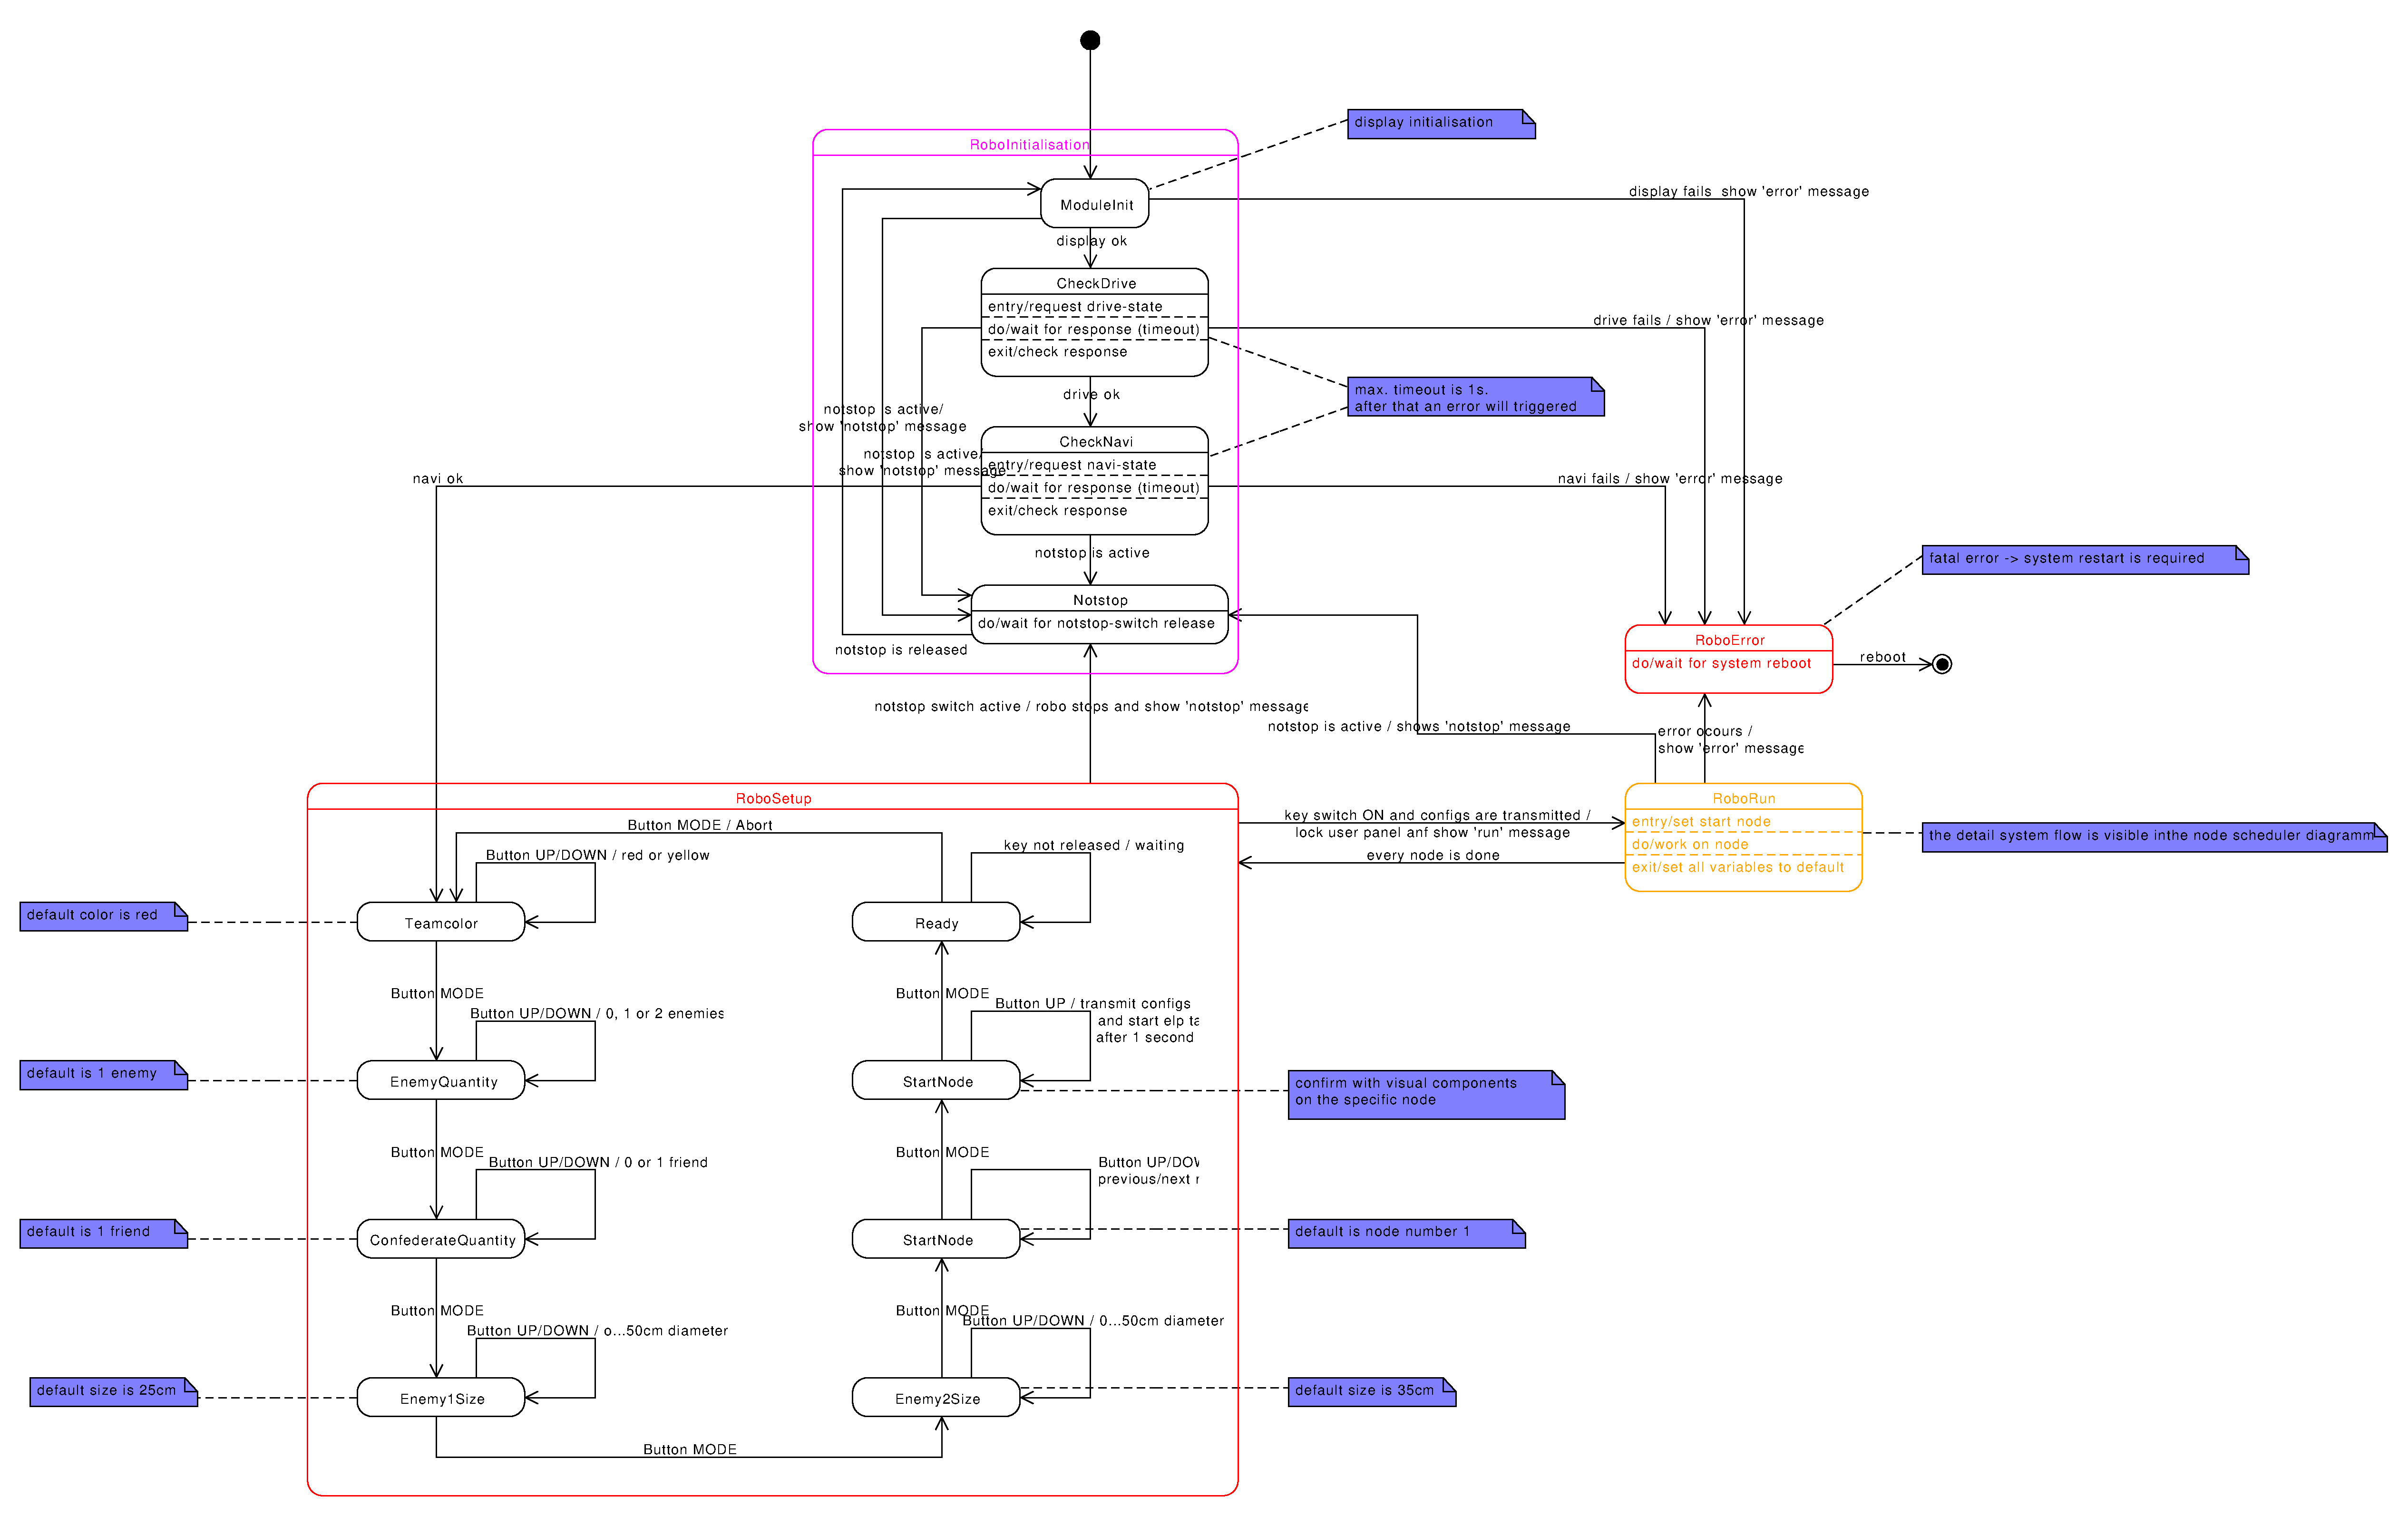
\includegraphics[angle=90,scale=0.26]{content/image/14_system_overview}
				\caption{Systemzust�nde}
				\label{pic:systemzust�nde}
			\end{figure}
			%
			\subsection{Match}\label{ss:match}
				Wie im \cref{s:speilstrategie} erkl�rt wird, besteht ein Match aus mehreren Spielaufgaben, die wiederum unterschiedlichen Konten in einem Graphen zugeordnet sind. F�r die Auswahl des n�chsten Knotens ist die Spielstrategie zust�ndig, f�r die Ausf�hrung der Knoten Task. Daf�r wird er vom System Task gesteuert und mit neuen Knotendaten informiert. Dieser Vorgang ist in der \cref{pic:match} verdeutlicht.
				%
				\image{content/image/14_node_scheduler}{scale=1}{htbp}[Knoten-Scheduling][pic:match]
				
	%
	%
	%Bedieneinheit
	\section{Bedieneinheit}\label{s:sw_bedieneinheit}
		Der f�r die Bedieneinheit entwickelte SW-Code ist grunds�tzlich in den folgenden Dateien zu finden:
		\begin{itemize}
			\item (spi.c/.h)
			\item display.c/.h
			\item RoboSetup.c/.h
		\end{itemize}
		%
		Dabei dienen die spi- und display-Dateien als Bibliotheksdateien (lib) und die RoboSetup-Datei als System-Datei (application/system). In der letztgenannten befindet sich die Men�-Steuerung um die gew�nschten Spiel-spezifischen Initialisierungen einzustellen.
		\par
		Die Konfigurationen erfolgen mit den drei Tastern unter dem Display. Die Taster links und rechts dienen der Auswahl einer Option und der mittlere Taster zur Best�tigung. S�mtliche Taster auf der Bedieneinheit funktionieren Flankengesteuert.
		%
		\subsection{SPI}\label{ss:spi}
			Diese Bibliotheksdatei wurden schlussendlich nicht mehr genutzt, da die Daten�bertragung manuell programmiert wurde. Sie beinhaltet jedoch eine SPI-Initialisierungsfunktion (initSPI()) und eine Send-Byte-Funktion (SPI\_send\_byte()), die mit den von stm32f4 gegebenen SPI-Funktionen realisiert wurde.\\
			Bei der Initialisierung ist zu beachten, dass lediglich die SCK- und MOSI-Pins konfiguriert werden. Das MISO-Pin wird in dieser Anwendung nicht ben�tigt, da nur vom Master (RoboBoard) zum Slave (Bedieneinheit) gesendet werden muss (send only).
			\par
			Bei den ersten Tests tauchte das Problem auf, dass die eingestellte Baudrate zu hoch war und daher mit dem Oszilloskop keine erkennbare Byte-�bertragung festgestellt werden konnte. Es ist daher darauf zu achten, dass der SPI\_BaudRatePrescaler gross genug gew�hlt wird. Er berechnet sich mit der Formel:
			\par
			$Baudrate = \frac{(APB2 frequency (=84MHz))}{Prescaler}$
			\par
			Verwendet wurde in einem zweiten Versuch der maximale Prescaler von 256, was eine Baudrate von 328'125 Hz zur Folge hat.\\
			Mit dieser Konfiguration funktionierte das erste Display. Das zweite f�r den grossen Roboter jedoch nicht. Da das Erste so weit zuverl�ssig lief, wurde der Fehler logischerweise in der HW gesucht. Nach aufw�ndiger Fehlersuche und der Mithilfe eines weiteren Kernteammitglieds (Simon) hat man die Fehlerquelle dennoch auf die SW begrenzen k�nnen. Dabei wurde versuchsweise die eingestellte �bertragungsfrequenz (mit einem Interrupt) auf 100 kHz begrenzt. Dieser Wert gilt z.B. f�r das im Kapitel \ref{sss:NHD} beschriebene Display (NHD-0216K3Z) als Maximalwert. Umgesetzt wurde dies mit einem Timerinterrupt in der display.c-Datei, in dessen Handler schlussendlich die gesamte Daten�bertragung umgesetzt wurde. Mit dieser Massnahme funktionierte auch das zweite Display.
			
			%Dem Datenblatt des Mikrocontrollers im Display (ST7036) kann man lediglich entnehmen, dass dessen interne Clock 540 kHz betr�gt.\\
			
			\par
			Bei einer �nderung der GPIO-Pins in der spi.h-Datei muss beachtet werden, dass allf�llig die Konfiguration des Peripherie-Clocks (RCC\_AHB1PeriphClockCmd()) in der spi.c-Datei angepasst werden muss.\todo{Anmerkung haldj: spi.c/h werden nicht mehr eingesetzt! Weiter nennt man die aktuelle Umsetzung Software-SPI. Zu erw�hnen w�re auch noch, dass die Sendefrequenz evtl. nicht die Ursache war, sonder den zum falschen Zeitpunkt eingesetzten RS-Pegel! Dies war auch der Hauptgrund zum Umschreiben der Software auf SW-SPI}
			%
		\subsection{Display}\label{ss:display}
			In dieser Bibliotheksdatei befinden sich s�mtliche Funktionen um das Display anzusteuern. Diejenigen die nicht verwendet wurden, werden in dieser Dokumentation nicht n�her erl�utert. Sie sollten jedoch selbsterkl�rend sein, da sie lediglich ein bestimmtes Instruktionsbyte ans Display senden und sinnvoll benannt wurden. Die wichtigsten Funktionen werden in der nachfolgenden Tabelle (\ref{tab:display-funktionen}) beschrieben:
	 		\begin{table}[H]
		    	\centering
		    	\caption{Display-Funktionen}
		    	\begin{tabular}{|p{3.5cm}|p{11cm}|} 
		    		\hline
		    		\rowcolor{bfhblue}
		    		\textcolor{white}{Funktion} & \textcolor{white}{Beschreibung} \\
					\hline
					LCD\_init() &  Initialisiert das RS-, SCK-, MOSI- und CS-Pin, den TIM2-Interrupt und das Display mit Hilfe der im Datenblatt des Displays beschriebenen Instruktionen\\
					\hline
					TIM2\_IRQHandler() & Interrupthandler der alle 10 us aufgerufen wird und mittelst einer statemachine die Daten�bertragung steuert\\ 
					\hline
					LCD\_write\_byte\_ instruction() & �bertr�gt ein Instruktionsbyte (RS = Low) um das Display zu steuern\\ 
					\hline
					LCD\_clear() & L�scht den Inhalt des Displays\\ 
					\hline
					LCD\_write\_byte\_ data() & �bertr�gt ein Datenbyte (RS = Hight)\\
					\hline
					LCD\_write\_string() & �bertr�gt mit Hilfe der LCD\_write\_byte\_data()-Funktion ein ganzer String\\
					\hline					
					LCD\_set\_cursor() & Setzt den Cursor (zu schreibender Zielort und/oder Marker) an der gew�nschten Stelle auf dem Display\\
					\hline						
					LCD\_set\_contrast() & Setzt den Kontrast des Displays mit einer Intensit�t zwischen 0 und 63, wobei 24 standardm�ssig eingestellt ist und im Normalfall nicht ver�ndert werden sollte\\
					\hline				
				\end{tabular}
			\label{tab:display-funktionen}
			\end{table}
			%
			Erw�hnenswert ist, dass bei der Kommunikation mit einem Display des �fteren Zeitverz�gerungen (delays) eingebaut werden m�ssen, damit der Controller des Displays Zeit f�r die Verarbeitung hat. Gel�st wurde dieses Problem mit der vTaskDelay()-Funktion von FreeRTOS die mittels einem Funktionspointer beim Aufruf der init\_display()-Funktion �bergeben wird und darin in eine private Variable (*Delay) gespeichert wird.
			\par
			Bei einer �nderung der GPIO-Pins in der display.h-Datei muss beachtet werden, dass allf�llig die Konfiguration des Peripherie-Clocks (RCC\_AHB1PeriphClockCmd()) in der display.c-Datei angepasst werden muss.
			%
		\subsection{RoboSetup}\label{ss:robosetup}
			In der RoboSetup-Datei befindet sich die Men�steuerung. Damit nicht aus Versehen Konfigurationen vergessen gehen, wurde ein serieller Aufruf der einzelnen Men�states realisiert (siehe Abbildung \ref{pic:menuabfolge}).\\
			Es wurde versucht ein m�glichst modularer Aufbau umzusetzen, damit wahlweise weitere Men�inhalte (Konfigurationen) hinzugef�gt werden k�nnen. Erreicht wurde dies mit dem typdef struct menu\_t (Abbildung \ref{pic:menu_t}). Pro ben�tigte Konfiguration (Men�state) muss somit zuerst je eine menu\_t-Struktur mit den gew�nschten Initialisierungswerten erstellt werden.
			\par
			\image{content/image/Bedienpanel/menu_t}{scale=0.8}{htbp}[Typdef structure menu\_t][pic:menu_t]
			%
			Damit die erstellten Men�inhalte dargestellt und die mit den Tastern eingestellten Konfigurationen gelesen werden k�nnen, wurden die in der folgenden Tabelle (\ref{tab:menu-funktionen}) beschriebenen Funktionen erstellt: 
	 		\begin{table}[H]
		    	\centering
		    	\begin{tabular}{|p{3.6cm}|p{11cm}|} 
		    		\hline
		    		\rowcolor{bfhblue}
		    		\textcolor{white}{Funktion} & \textcolor{white}{Beschreibung} \\
					\hline
					initRoboSetupState() &  Definiert den ersten Men�state und ruft die initUserPanelButtons()-Funktion auf, die in der Datei button.c/.h programmiert wurde. Da sie analog s�mtlicher RoboBoard-Buttons funktionieren, wird an dieser Stelle nicht n�her darauf eingegangen\\
					\hline
					runRoboSetupState() & Enth�lt die Statemachine, die die einzelnen Men�inhalte (Men�states) aufrufen und kontrollieren. Die genaue Abfolge ist in der Abbildung \ref{pic:menuabfolge} zu sehen\\ 
					\hline
					write\_current\_menu() & Gibt mit der Hilfe der display-Funktionen den momentan aktuellen Men�state auf das Display aus\\ 
					\hline
					menu\_handler() & Beinhaltet die eigentliche Men�steuerung. Es werden die einzelnen Taster abgefragt und die aktuell ausgew�hlten Resultate abgespeichert\\ 
					\hline
					setConfigRoboSetup-2Default() & Setzt die einzelnen Men�s auf die in der RoboSetup.h definierten Default-Werte zur�ck. Dies wird bei einem Reset des Roboters (z.B. nach einem Notstop) ben�tigt\\
					\hline								
				\end{tabular}
			\caption{Men�-Funktionen}
			\label{tab:menu-funktionen}
			\end{table}
			%
			\par
			\image{content/image/Bedienpanel/menuabfolge}{scale=1}{htbp}[Men�abfolge der Statemachine][pic:menuabfolge]
			%
			In der menu\_handler()-Funktion muss nebst dem momentan aktuellen Men� (menu\_t) die ausw�hlbaren Resultate �bergeben werden. Ausserdem muss zwischen zwei Men�typen unterschieden werden: SELECTION\_MENU und ADJUSTING\_MENU.
			\par
			Ein SELECTION\_MENU kann zwischen maximal drei Optionen unterscheiden, wobei eine davon ausgew�hlt werden kann. Zum Beispiel bei der Auswahl der Anzahl der gegnerischen Roboter (0, 1 oder 2).
			\par
			Ein ADJUSTING\_MENU enth�lt nur eine Option (opt2) die jedoch vergr�ssert oder verkleinert werden kann. Zum Beispiel bei der Konfiguration der H�he der gegnerischen Roboter (0 bis 50cm).
			%
	%
	%Spielstrategie
	\section{Spielstrategie}\label{s:speilstrategie}
		Eine gute Spielstrategie entscheidet schlussendlich �ber Sieg oder Niederlage. Deshalb wird ein grosses Augenmerk auf eine ausgefeilte Spielstrategie gelegt.
		%
		%Anforderungen
		\subsection{Anforderungen}\label{ss:anforderungen}
			Ein Roboter kann w�hrend einer Spielrunde in viele unvorhersehbare Situationen kommen, in denen er m�glichst angemessen handeln muss. Gleichwohl sollte er nicht nur reagieren, sondern auch agieren und damit m�glichst viele Punkte sammeln. Die folgenden Aufz�hlung zeigt was eine Spielstrategie erf�llen muss.
			%
			\begin{itemize}
				\item Spielaufgaben mit h�herem Punktegewinn bevorzugen
				\item Distanzen und damit den Zeitaufwand zwischen den einzelnen Spielaufgaben ber�cksichtigen
				\item Zeitaufwand f�r eine Spielaufgabe beachten
				\item Position des/der Gegners/Gegner einbeziehen
				\item Selbst�ndig, mit Ber�cksichtigung der bisher aufgef�hrten Punkten, die n�chste Spielaufgabe evaluieren
				\item Der Algorithmus muss so ausgelegt sein, dass eine zyklische Ausf�hrung (im Bereich von 1Hz) m�glich ist. 
			\end{itemize}
		%
		%Idee
		\subsection{Idee}\label{ss:idee}
			In der Algorithmik im Zusammenhang mit Robotnik st�sst man auf zwei weit verbreitete L�sungsm�glichkeiten um einen Weg von A nach B zu finden. Der eine Ansatz h�rt auf den Namen \gls{g:astar} und der andere nennt sich das \gls{g:tsp}. Gemeinsam habe beide Methoden, dass sie auf der Graphentheorie aufbauen.
			%
			\subsubsection{Graphentheorie}
				Um die Funktionsweise der beiden Algorithmen verstehen zu k�nnen, ist es zwingend notwendig die Grundlagen der Graphentheorie verstanden zu haben. Ein Graph ist eine Ansammlung von Knoten, die via Kanten miteinander verbunden sind. Die Definition eines Graphen lautet $$G=(V,E)$$ wobei $V=\{1,2,...,n\}$ die Knotenmenge und $E:=V\times V$ die Kantenmenge darstellt. Weiter ist ein Graph meist gewichtet, was eine Kostenfunktion $c:E\rightarrow\mathbb{N}$, die jeder Kante $(i,j)$ ein Gewicht zuordnet, zur Folge hat \cite[S.2]{lit:tsp_achen}.\par 
				%
				Es wird zwischen verschiedenen Graphentypen unterschieden. Einfluss auf das finden einer Spielstrategie haben die Typen symmetrischer / ungerichteter Graph und unsymmetrischer/gerichteter Graph.
				%
				\begin{description}
					\item[symmetrischer Graph] Bei einem symmetrischen Graphen sind die Gewichte der Kanten unabh�ngig von der Richtung in der sie durchlaufen werden. Soll heissen $c(i,j) = c(j,i)$.
					%
					\item[asymmetrischer Graph] Im Gegensatz zum symmetrischen Graphen spielt die Richtung zwischen zwei Knoten eine entscheidende Rolle. Es gilt $c(i,j) \neq c(j,i)$.  
					%
					\item[vollst�ndiger Graph] Ein Graph wird als vollst�ndig bezeichnet, wenn alle Knoten via Kanten miteinander verbunden sind.
				\end{description}
			%
			\subsubsection{\gls{g:astar}}
				Der \gls{g:astar}-Algorithmus ist ein informierter Suchalgorithmus, der das Ziel hat den k�rzesten Pfad zwischen zwei Knoten zu finden. Es ist ein optimaler Algorithmus, soll heissen, es wird immer der k�rzeste Pfad gefunden (wenn vorhanden)\cite{lit:astar_wiki}. \par 
				Eine Bedingung an die Spielstratgie ist es selbst�ndig die n�chste Spielaufgabe zu finden (siehe \cref{ss:anforderungen}). Durch die Gegebenheit das der \gls{g:astar}-Algorithmus ein bekanntes Ziel braucht um einen Pfad zu bestimmen, ist er daher nicht f�r die vorliegende Aufgabe geeignet (n�chstes Ziel unbekannt).
			%
			\subsubsection{\gls{g:tsp}}\label{sss:tsp}
				Das \gls{g:tsp} ist ein kombinatorisches Optimierungsproblem der theoretischen Informatik. Es geht darum, dass ein Handelsreisender eine gewisse Anzahl St�dte besuchen und gleichzeitig den daf�r notwendige Zweitaufwand minimieren m�chte. Um dies zu erreichen, darf er jede Stadt nur einmal besuchen und muss weiter den optimalen Weg zwischen den St�dten finden \cite[S.1]{lit:tsp_achen}.\par 
				F�r das Aufstellen des \gls{g:tsp} muss ein vollst�ndiger Graph vorhanden sein. Ein Startpunkt oder Endpunkt ist nicht zwingend notwendig. Dieser Umstand pr�destiniert diesen Ansatz f�r eine erfolgreiche Spielstrategie.
		%
		%Problem des Handlungsreisenden 
		\subsection{\gls{g:tsp}}\label{ss:tsp}
			Beim \gls{g:tsp} handelt sich um ein sogenanntes NP-vollst�ndiges Problem \cite{lit:np}. Dies bedeutet, dass die Worst-Case Laufzeit jedes deterministischen Algorithmus mindestens exponentiell von der Anzahl Knoten abh�ngt. Dieser Umstand ist entscheidend beim finden einer effizienten Rundreise, genannt Hamiltonkreis im Graphen $G$, da nur beschr�nkt Rechenleistung zur Verf�gung steht.\par 
			%
			Durch die NP-Vollst�ndigkeit des Problems ist die Anzahl m�glicher L�sungen proportional zu $n!$, wobei $n$ die Anzahl Knoten darstellt. Im Falle eines symmetrischen Graphens ergibt sich daraus $\frac{(n-1)!}{2}$ m�gliche L�sungen. Der Umstand der Symmetrie ist im vorliegenden Problem jedoch nicht gegeben, da der Aufbau des kleinen Roboters asymmetrisch ist (Schussvorrichtung befindet sich auf der linken Seite) und es daher eine Rolle spielt von welcher Richtung die Konten angefahren werden. Die Anzahl m�glicher L�sungen erh�ht sich dadurch um den Faktor 2 (ingesamt $(n-1)!$ L�sungen).\par 
			%
			Ein Rundreise in einem Graphen kann auf unterschiedliche weise gefunden werden. Die Unterschiede der Methoden reduzieren sich auf die Laufzeit und ihre Exaktheit. In den Abschnitten \ref{sss:brute_force} bis \ref{sss:neighbour} werden gel�ufige Ans�tze aufgezeigt. 
			%
			\subsubsection{Brute-Force Methode}\label{sss:brute_force}
				Die Brute-Force Methode stellt eine exakte L�sungsm�glichkeit des Problems dar. Diese M�glichkeit verfolgt den Ansatz alle vorhanden Routen zu berechnen und die effizienteste als L�sung zu markieren. Durch die in \cref{ss:tsp} erkl�rte NP-Vollst�ndigkeit des Problems hat dies einen exponentiellen Zeitaufwand zur Folge. Dieser Fakt macht diese Methode unbenutzbar, ist doch einer der Anforderungen einen kurze Laufzeit\footnote{F�r 20 Knoten (asym. Graph) braucht ein Computer, der pro Sekunde $10^{24}$ L�sungen generiert, 121ns. F�r 30 Knoten sind es bereits 102 Tage \cite[S.11]{lit:tsp_achen}} des Algorithmus (siehe \cref{ss:anforderungen}).
			%
			\subsubsection{MST-\gls{g:heuristik}}
				Erf�llt der Graph die Punkte
				%
				\begin{itemize}
					\item $c(i,j)\geq0$ f�r alle $i,j\epsilon V$ und $c(i,j)=0$ wenn $i=j$
					\item $c(i,j)=c(j,i)$ (Symmetrie)
					\item $c(i,j)+c(j,k) \geq c(i,k)$ (Dreiecksungleichung)
				\end{itemize}
				%
				so handelt es sich um eine metrisches \gls{g:tsp}. Der Vorgang um Reiserouten mit Hilfe eines Minimum-Spanning-Trees zu finden, beinhaltet die folgenden Schritten \cite[S.14]{lit:tsp_achen}:
				\begin{enumerate}
					\item Minimaler Spannungsbaum $T$ aufziehen mit den Algorithmen von Prim oder Kruskall
					\item Jeder Kante verdoppeln in $T$
					\item Einen Startknoten $v$ bestimmen $T$
					\item Eulerkreis $K$ in $T$ ermitteln
					\item Im Eulerkreis alle Kanten entfernen, die bereits zu einem besuchten Knoten f�hren und ersetze sie durch eine Kante zu einem Konten, der im Eulerkreis an n�chster Stelle kommt (ausser Startknoten). 
				\end{enumerate}	
				Die sich dadurch ergebende Route ist maximal um den Faktor 2 l�nger als die optimale. Da die Punkte der Symmetrie und Dreieckungleichung vom vorliegenden Problem nicht erf�llt werden, kann diese Heuristik nicht eingesetzt werden. 	
			%
			\subsubsection{Nearest-Neighbour \gls{g:heuristik}}\label{sss:neighbour}
				Bei der Nearest-Neighbour Heuristik handelt es sich um einen Greedy-Algorithmus, was so viel bedeutet, dass er lokale optimale L�sungen findet, die schlussendlich zu einer globalen L�sung f�hren. Dadurch ist dieser Ansatz jedoch nicht sehr vorausschauend, daf�r relativ einfach umzusetzen.
				%
				\begin{enumerate}
					\item Alle Knoten als unbesucht kennzeichnen
					\item Einen Startknoten w�hlen
					\item Knoten $v$ finden, der mit einem minimalen Gewicht vom Startknoten aus erreichbar ist.
					\item Den Knoten $v$ als besucht markieren
					\item Die Schritte 3 bis 4 so lange wiederholen bis alle Knoten als besucht gekennzeichnet sind 
				\end{enumerate}
				%
				Dieser Ansatz ist sehr zeiteffizient, kann jedoch als Resultat die schlechtest m�gliche Handelsroute liefern \cite[S.12]{lit:tsp_achen}. Durch seine Einfachheit ist er jedoch pr�destiniert f�r den Einsatz auf einem eingebetteten System. Weiter kann er auch bei asymmetrische Grahpen eingesetzt werden, weshalb diese Heuristik gew�hlt wird.   	
		%
		%Konzept
		\subsection{Konzept}\label{ss:konzept}
			Mit dem erkorenen Ansatz \gls{g:tsp} und dem bestimmten Algorithmus Nearest-Neighbour \gls{g:heuristik} wird in den folgenden Abschnitten ein Konzept bezogen auf die Spielstrategie des kleinen Roboters entworfen. Dabei gilt es die zentralen Punkte des Gewichtung der Knoten und deren Variationen zu behandeln. F�r den Entwurf und die Validierung wird zum einem Matlab eingesetzt und zum anderen die reale Spielumgebung (Roboter + Spielfeld).
			%
			\subsubsection{Graph und Spielfeld}
				Die Knoten des f�r das \gls{g:tsp} n�tigen Graphen m�ssen auf das gegebene Spielfeld adaptiert werden. Dabei soll jeder Knoten eine Spielaufgabe repr�sentieren. Im Falle des kleinen Roboter sind dies die Aufgaben \gls{g:fresko}, \gls{g:fire} und \gls{g:mammut}. Um die Strategie dynamisch zu gestalten, gibt es, wenn m�glich, mehrere Knoten pro Aufgaben. Somit kann w�hrend des Match derjenige Knoten einer Aufgabe gel�st werden, der den gr�ssten Erfolg verspricht. In der \cref{pic:spielfeld_knoten} sind die Knoten, 11 an der Zahl (ohne den gelben Startpunkt), ersichtlich. Dabei stellen die blau umrahmten Knoten Abschusspositionen f�r die Aufgabe \gls{g:mammut} dar. Die magentafarbenen  Rahmen Kennzeichnen Klebepunkte der Aufgabe \gls{g:fresko}. Die �brigen, nicht umrahmten, Knoten lokalisieren Punkte an denen ein Feuer umgekippt werden kann (Aufgabe \gls{g:fire}). 
				%
				\image{content/image/14_field_node_pools_red}{scale=1.2}{htbp}[Knoten auf dem Spielfeld (Teamfarbe rot)][pic:spielfeld_knoten]
				%
				
			%
			\subsubsection{Knotengewichtung}
				Massgebend f�r einen brauchbaren Graphen ist eine geschickte Gewichtung der Knoten. Diese besteht aus den Komponenten:
				%
				\begin{itemize}
					\item Kosten eines Knoten
					\begin{itemize}[parsep=1pt, topsep=-10pt]
						\item M�gliche Punkte
						\item Zeit bis zum erf�llen des Knoten
						\item Prozentualer Anteil an der gesamt Punktzahl
						\item Anfahrtsrichtung des Knoten (asymmetrischer Roboter)
					\end{itemize}
					\item Fahrzeit zum Knoten
					\item Vergangene Positionen des Gegners (falls sich der Gegner lange in der N�he eines Knoten aufh�lt, so ist die Chance gross, dass diese Aufgabe bereits durch den Gegner gel�st wurde) 
				\end{itemize}
				%
				\paragraph{Komponenten Gewichtung} Nicht alle dieser zuvor aufgef�hrten Komponenten haben jederzeit w�hrend des Matchs die gleiche Bedeutung. So ist die Fahrzeit zu Beginn, wenn noch gen�gend Zeit vorhanden ist, nicht weiter von Bedeutung. Dagegen w�re es sinnvoll am Anfang m�glichst Aufgaben mit grossem Punkteertrag zu l�sen. Umgekehrt verh�lt es sich gegen Ende des Matchs. Zu diesem Zeitpunkt interessiert nur noch die Fahrzeit und nicht wie viel Punkte ein Knoten ergeben k�nnte. Daher werden die einzelnen Komponenten positiv oder negativ linear gewichtet. Die Gewichtung erfolgt dabei in Abh�ngigkeit der Zeit, ersichtlich in der \cref{eq:gewichtung}.\par
				%
				\formula{
				    &w_{inc} = \frac{t_{current}}{t_{Game}}\\
				    &w_{dec} = \frac{t_{Game}-t_{current}}{t_{Game}}
				}{
				    w_{inc} & Gewichtung zunehmend [0 1]\\
				    w_{dec} & Gewichtung abnehmend [0 1]\\
				    t_{Game} & Spielzeit 90 Sekunde\\
				    w_{dec} & Aktuelle Zeit [0 90]}[eq:gewichtung]
				%
				\paragraph{Anfahrtsrichtung} F�r die Ber�cksichtigung der Anfahrtsrichtung des Knoten wird die Komponente \textsf{Kosten eines Knoten} zus�tzlich ganzzahlig mit einem Faktor 1 bis 4 multipliziert. Der Faktor 1 entspricht dabei einer optimalen Anfahrt. Die verschiedenen Anfahrtszonen sind der \cref{pic:anfahrt} zu entnehmen. Es wird zwischen 
				%
				\begin{enumerate}
					\item optimale Anfahrt (Fakor 1)
					\item gute Anfahrt, seitlich (Faktor 2)
					\item normale Anfahrt, zu nahe beim Knoten, gleiche H�he (Faktor 3)
					\item schlechte Anfahrt, auf der gegen�berliegenden Seite (Faktor 4)
				\end{enumerate}
				%
				unterschieden. Der Abstand \textsf{Frame} kann eingestellt werden und betr�gt standardm�ssig 15cm.\par 
				%
				\image{content/image/14_node_arrive}{scale=0.4}{htbp}[Anfahrtsrichtung-Gewichtung (Anfahrt aus Norden)][pic:anfahrt] 
				%
				\paragraph{Gegner Tracking} Da der Roboter �ber keine visuellen Sensoren verf�gt, mit denen das Vorhanden sein eines Spielelements gepr�ft werden kann, muss die Position des Gegners aufgezeichnet werden. Mit dieser Aufzeichnung kann anschliessend abgesch�tzt werden, ob eine Aufgabe bereits gel�st wurde.\par
				%
				Das Tracking wird auf einer sehr einfache weise umgesetzt. Jede empfangene Position eines Gegners wird in einer Gitter-Map mit einer Gewichtung vermerkt. Da die Positionserkennung einer gewissen Ungenauigkeit unterliegt, wird um die effektiv erhaltene Position einen Rahmen mit einer tieferen Gewichtung gelegt\footnote{Die H�he der Zentrum-/Rahmen-Gewichtung muss w�hrend den Tests eventuell modifiziert werden. Aktuell liegen sie bei 3, respektive 4}. Falls eine Position mehrmals empfangen wird, so wird das Gewicht mit dem bereits bestehenden aufaddiert. Ein m�gliches Tracking-Resultat zeigt die \cref{pic:tracking}.
				%
				\image{content/image/14_enemy_track_red}{scale=0.8}{htbp}[Gegner-Tracking einer m�glichen Route][pic:tracking]
				%
				\paragraph{Totales Kontengewicht}Das totale Gewicht eines Knoten berechnet sich anschliessend wie in \cref{eq:w_node} ersichtlich. Je tiefer das Gewicht ausf�llt, des h�her ist der Wert des Knoten.
				%
				\formula{
					w_{Node}&=w_{dec}*c_{dest}+w_{dec}*c_{enemy}\\
					&+w_{inc}*c_{src/dest}
					}{
					w_{Node} & Gewicht des gesamten Knoten\\
					c_{dest} & Kosten des Knoten\\
					c_{enemy} & Kosten vergangene Gegner-Positionen\\
					c_{src/dest} & Kosten Fahrzeit\\
					w_{inc} & Gewichtung zunehmend [0 1]\\
					w_{dec} & Gewichtung abnehmend [0 1]}[eq:w_node]
				%
			%
			\subsubsection{Gruppierung von Knoten}
				Der kleine Roboter hat die M�glichkeiten
				%
				\begin{itemize}
					\item 3x 2 B�lle abzufeuern.
					\item 1x 2 Fresko zu kleben.
					\item 3x 1 Feuer umzukippen.
				\end{itemize}
				%
				Um der Strategie m�glichst grossen Freiraum zu bieten, werden mehre Knoten f�r dieselbe Aufgabe definiert (z.B. 6 Abschusspositionen f�r die B�lle anstatt der 3 n�tigen). Dieser Umstand kann in der \cref{pic:spielfeld_knoten} nachvollzogen werden. Dabei sind die zusammenh�ngenden Knoten stets gleichfarbig umrahmt. Eine Gruppe von Knoten wird als Pool bezeichnet. Im Graphen des kleinen Roboters sind somit 2 Pools vorhanden.\par 
				%
				Jedes Pool besteht aus einer gewissen Anzahl von Knoten und einem zuvor definierten Pool-Level. Dieses Level kennzeichnet die Anzahl abzuarbeitenden Knoten, die f�r die Erf�llung des Pools n�tig sind. Ist ein Pool als abgeschlossen markiert, so werden alle �brigen Knoten des Pools ebenfalls als erledigt betrachtet.
				
			%
			\subsubsection{Ablauf}\label{sss:ablauf_strategie}
				Das Vorgehen um von einem Knoten $x$ den n�chsten Knoten $y$ auszumachen gestaltet sich, dank des Nearest-Neighbour Ansatzes, sehr effizient und einfach. Es muss lediglich das Gewicht jedes Knotens (darf noch nicht erledigt sein) ermittelt und mit den anderen Gewichten verglichen werden. Damit erh�lt man schlussendlich den Knoten mit der tiefsten Gewichtung, was gleichbedeutend mit dem n�chste zu erledigen Knotens ist. Die \cref{pic:ablauf_knoten} illustriert dieses Vorgehen. 
				%
				\image{content/image/14_ablauf_strategie}{scale=0.4}{htbp}[Ablauf Knotenbestimmung][pic:ablauf_knoten]
		%
		%Spielablauf
		\subsection{Spielablauf}\label{ss:spielablauf}
			Der vorliegende Abschnitt zeigt das zuvor in \cref{ss:konzept} erstellte Konzept in einer Matlab-Simulation angewandt. Dabei herrschten die folgend aufgef�hrten Bedingungen vor:
			%
			\begin{itemize}
				\item Teamfarbe rot
				\item 1 eigener Roboter mit den Aufgabe \gls{g:mammut}, \gls{g:fresko} und \gls{g:fire}
				\item kein gegnerischer Roboter
			\end{itemize}
			%
			\paragraph{Match-Start}Am Anfang einer Partie muss festgelegt werden, welcher Knoten zuerst behandelt werden soll. Nach dem erf�llen dieses Knotens sucht der Stratgie-Algorithmus (siehe \cref{sss:ablauf_strategie}) selbstst�ndig den n�chsten. F�r die Identifizierung der Knoten wird jedem einen ID zugeordnet. Je nach Teamfarbe k�nnen sich diese unterscheiden, wie die \cref{abb:node_id} zeigt.\par 
			\begin{figure}[htbp] %htbp
				\centering
				\begin{subfigure}[b]{0.49\textwidth}
					\centering
					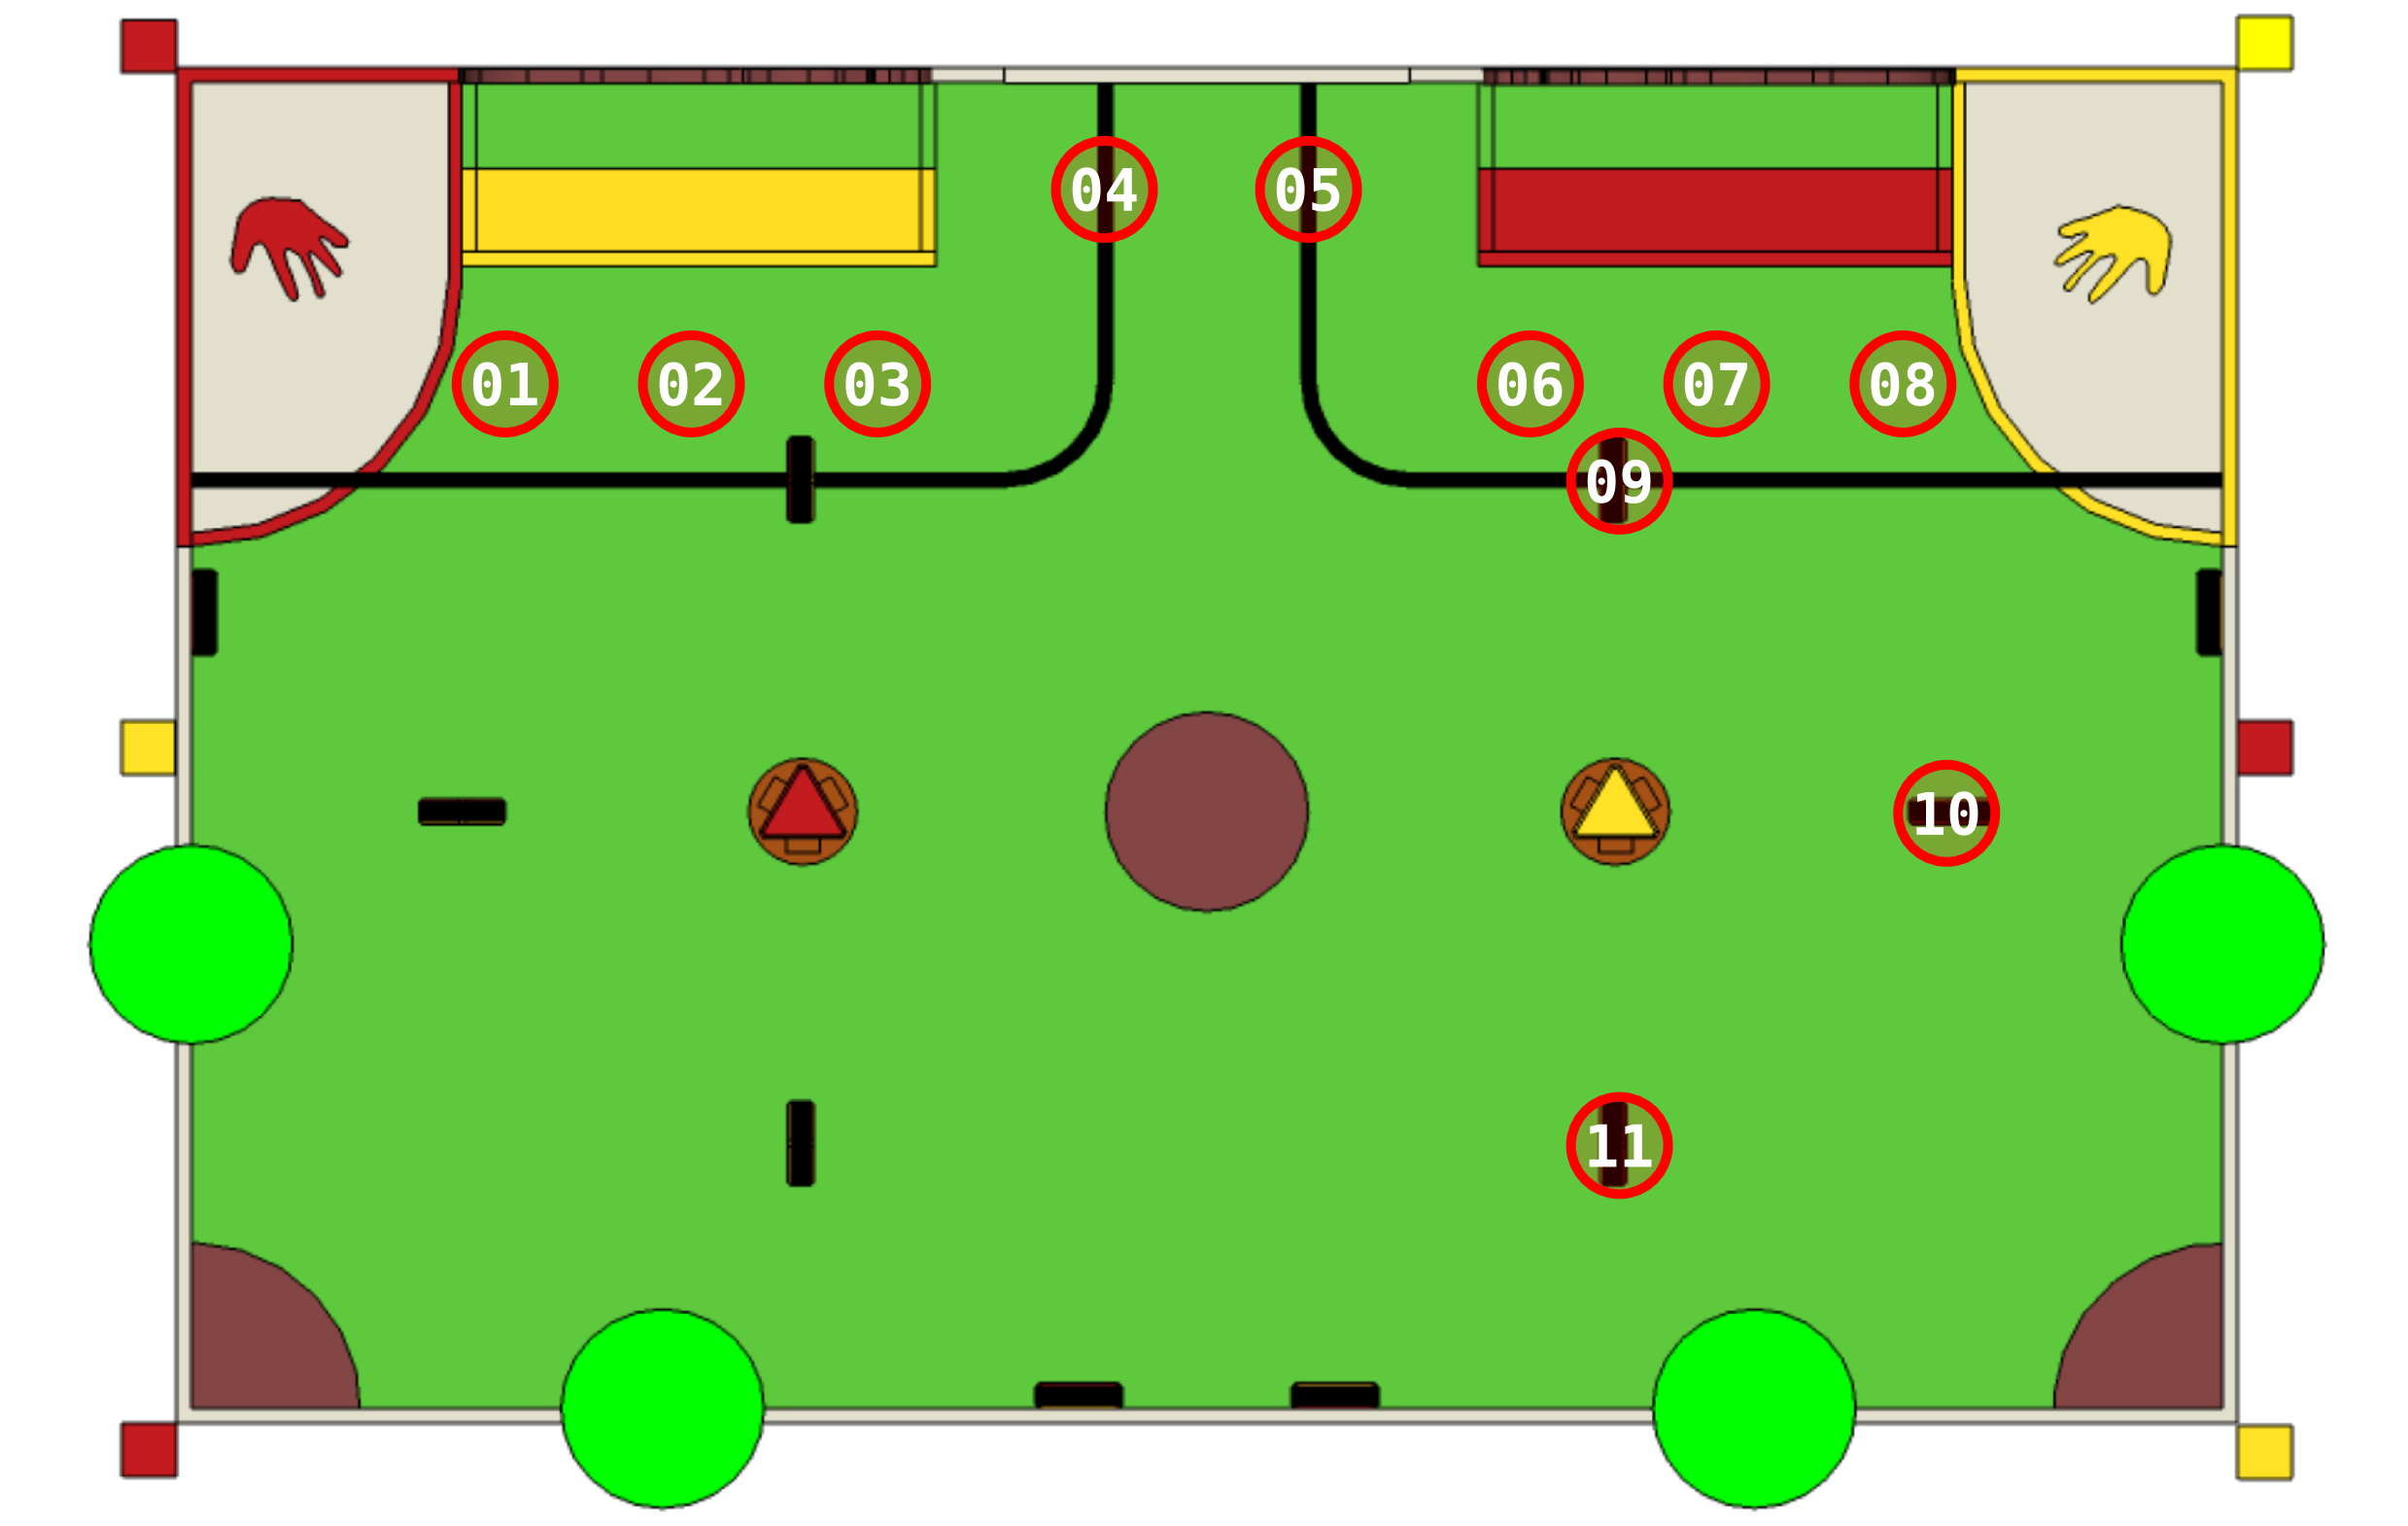
\includegraphics[height=4.95cm]{content/image/14_knoten_IDs_red_small}       
					\caption{Teamfarbe rot}
				\end{subfigure}
				\begin{subfigure}[b]{0.49\textwidth}
					\centering
					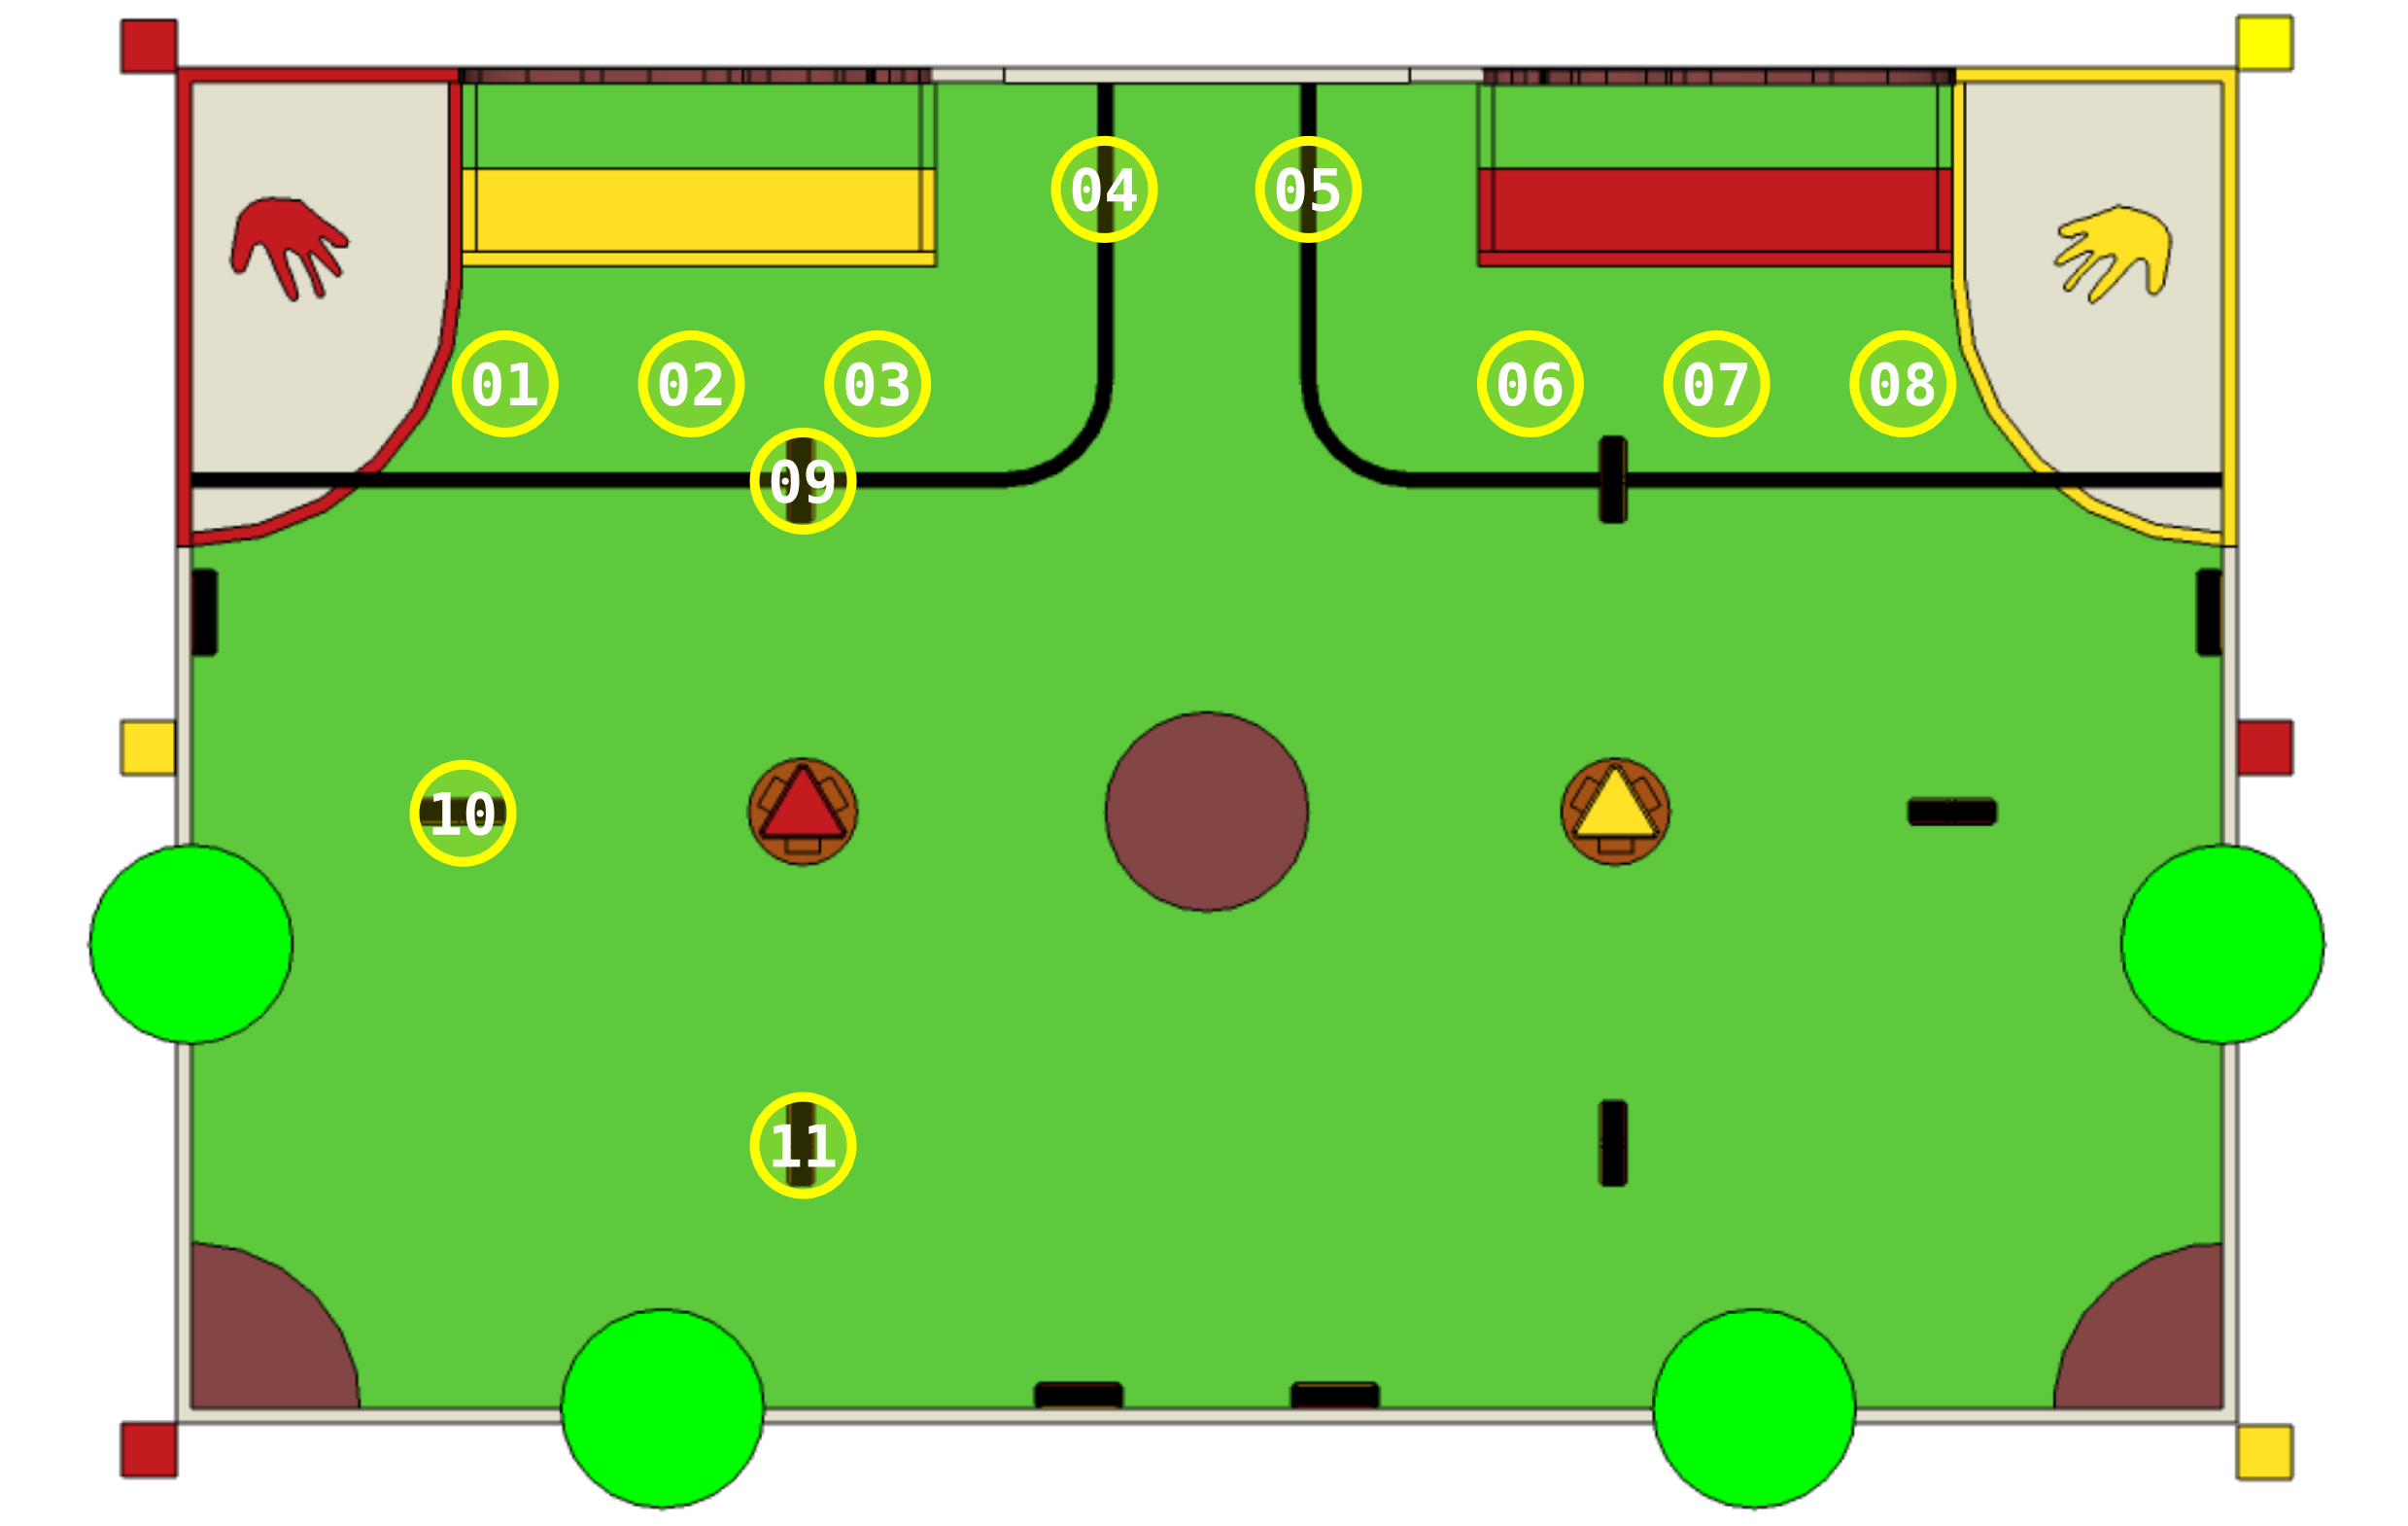
\includegraphics[height=4.95cm]{content/image/14_knoten_IDs_yellow_small}    
					\caption{Teamfarbe gelb}     
				\end{subfigure}
				\caption{Knoten ID's}
				\label{abb:node_id}
	    	\end{figure}
	    	%
	    	Ist der Startknoten ausgew�hlt und der Match gestartet, so pr�sentiert sich die Situation wie in \cref{pic:match_start} dargestellt. Der gr�n markierte Knoten referenziert dabei den Startknoten.
	    	%
	    	\image{content/image/14_field_node_pools_red}{scale=0.6}{htbp}[Spielfeldsituation bei Match-Start Teamfarbe rot][pic:match_start]
	    	%
	    	\paragraph{Match-Ende} Am Ende eines Matchs sollten alle Knoten abgearbeitet sein. Ist dies der Fall, so ist eine m�gliche Route der Strategie in der \cref{pic:match_ende} ersichtlich (gr�ne Linien).\par 
	    	%
	    	\image{content/image/14_field_end_red}{scale=0.6}{htbp}[Spielfeldsituation bei Match-Ende Teamfarbe rot][pic:match_ende]
	    	%
			Der Knoten-Gewicht-Verlauf �ndert w�hrend der gesamten Match-Dauer in Abh�ngigkeit des aktuellen Knotens (siehe \cref{pic:match_weight}). Zu beachten ist, dass dieses Diagramm ohne Ber�cksichtigung eines Gegners aufgezeichnet wurde. Ein allf�lliger Gegner w�rde eine Horizontaltverschiebung nach oben des Gewichtsverlaufes zur Folge haben. Weiter kann im Diagramm der Wert einzelner Spielaufgaben erkannt werden. Die Aufgaben \gls{g:mammut} und \gls{g:fresko} liegen sehr nahe beieinander, wohingegen die Aufgabe \gls{g:fire} zu Beginn kaum ins Gewicht f�llt.
	    	%
	    	\image{content/image/14_weight_end_red}{scale=0.6}{htbp}[Knoten-Gewichte w�hrend eines Matchs][pic:match_weight]
	    	
		
			
	%
	%
	%Spielaufgaben
	\section{Spielaufgaben}\label{s:spielaufgaben}{kasen1}
		
%
%Kapitel 7: Validierung
%%%%%%%%%%%%%%%%%%%%%%%%%%%%%%%%%%%%%%%%%%%%%%%%%%%%%%%%%%%%%%%%%%%%%%%%%%%%%%%%
% Titel:   Testkonzept
% Autor:   
% Datum:   15.01.2014
% Version: 0.0.2
%%%%%%%%%%%%%%%%%%%%%%%%%%%%%%%%%%%%%%%%%%%%%%%%%%%%%%%%%%%%%%%%%%%%%%%%%%%%%%%
%
%:::Change-Log:::
% Versionierung erfolgt auf folgende Gegebenheiten: -1. Release Versionen
%                                                   -2. Neue Kapitel
%                                                   -3. Fehlerkorrekturen
% 0.0.2       Text und Kapitel hinzugef�gt.
% 0.0.1       Erstellung der Datei
%%%%%%%%%%%%%%%%%%%%%%%%%%%%%%%%%%%%%%%%%%%%%%%%%%%%%%%%%%%%%%%%%%%%%%%%%%%%%%%    
\chapter{Testkonzept PA2}\label{ch:validierung_pa2}

	%
    %Review Test
    \section{Review Test}\label{s:review_test_pa2}
%    	Der Review Test wird f�r jedes Modul einzeln durchgef�hrt. Dabei soll darauf geachtet werden, dass nicht der Verantwortliche des jeweiligen Moduls den Review Test selber durchf�hrt. Anschliessend an den Test, werden die nicht erf�llten Punkte vom Modulzust�ndigen korrigiert. Der Review Test ist in vier Teile gegliedert:
%    	%
%   		\begin{description}
%   			\item[Kommentark�pfe] Beinhaltet alle Tests bez�glich der Header- und Funktionsk�pfe.
%   			%
%   			\item[Namensgebung] In diesem Abschnitt werden die Code-Richtlinien, die zu Beginn des Projekts festgelegt wurden.
%   			%
%   			\item[Kommentar] Hier wird der Kommentar auf die festgelegten Richtlinien getestet.
%   			%
%   			\item[Kommentarstil] Beim Kommentarstil wird einerseits darauf geachtet, ob der Kommentar sinnvoll ist und ob er verst�ndlich ist, andererseits wird auch die Formatierung noch ein wenig angeschaut.
%   		\end{description}
    %
    %Funktionstest
    \section{Funktionstest}\label{s:funktionstest_pa2}
%    	Im Gegensatz zum Review Test wurde nur ein Funktionstest f�r das gesamte Projekt entworfen. Der Funktionstest ist zum momentanen Zeitpunkt in vier Kategorien unterteilt:
%    	%
%   		\begin{description}
%   			\item[Bilderkleben] Beinhaltet alle Test, die zur erfolgreichen Ablauf des Bilderklebens n�tig sind.
%   			%
%   			\item[Ballspicken] Test die den reibungslosen Vorgang des Ballspickens gew�hrleisten sollen. 
%   			%
%   			\item[CAN Test] In diese Kategorie geh�ren alle Tests, die die Kommunikation zwischen den einzelnen Knoten im Roboter sicherstellen.
%   			%
%   			\item[Gesamttests] Am Ende wird ein Gesamttest durchgef�hrt um auch das Zusammenspiel der einzelnen Komponenten testen zu k�nnen.
%   		\end{description}
%    	%
%
%Kapitel 8: Ergebnisse
%%%%%%%%%%%%%%%%%%%%%%%%%%%%%%%%%%%%%%%%%%%%%%%%%%%%%%%%%%%%%%%%%%%%%%%%%%%%%%%%
% Titel:   Ergebnis
% Autor:   
% Datum:   22.09.2013
% Version: 0.0.1
%%%%%%%%%%%%%%%%%%%%%%%%%%%%%%%%%%%%%%%%%%%%%%%%%%%%%%%%%%%%%%%%%%%%%%%%%%%%%%%
%
%:::Change-Log:::
% Versionierung erfolgt auf folgende Gegebenheiten: -1. Release Versionen
%                                                   -2. Neue Kapitel
%                                                   -3. Fehlerkorrekturen
%
% 0.0.1       Erstellung der Datei
%%%%%%%%%%%%%%%%%%%%%%%%%%%%%%%%%%%%%%%%%%%%%%%%%%%%%%%%%%%%%%%%%%%%%%%%%%%%%%%    
\chapter{Ergebnis}\label{ch:ergebnis_pa2}
%
%Kapitel 9: Schlussfolgerung
%%%%%%%%%%%%%%%%%%%%%%%%%%%%%%%%%%%%%%%%%%%%%%%%%%%%%%%%%%%%%%%%%%%%%%%%%%%%%%%
% Titel:   Schlusswort
% Autor:   
% Datum:   22.09.2013
% Version: 0.0.1
%%%%%%%%%%%%%%%%%%%%%%%%%%%%%%%%%%%%%%%%%%%%%%%%%%%%%%%%%%%%%%%%%%%%%%%%%%%%%%%
%
%:::Change-Log:::
% Versionierung erfolgt auf folgende Gegebenheiten: -1. Release Versionen
%                                                   -2. Neue Kapitel
%                                                   -3. Fehlerkorrekturen
%
% 0.0.1       Erstellung der Datei
%%%%%%%%%%%%%%%%%%%%%%%%%%%%%%%%%%%%%%%%%%%%%%%%%%%%%%%%%%%%%%%%%%%%%%%%%%%%%%%    
\chapter{Schlusswort}\label{ch:schlusswort_pa2}
	Am Schluss der \gls{ac:pa2} sind wir immer noch zuversichtlich, dass wir an den nationalen Ausscheidungen in Burgdorf erfolgreich teilnehmen werden. Der Projektstand ist zwar rund eine Woche in R�ckstand und es gibt noch vieles zu erledigen, jedoch ist die Motivation bei den Teammitgliedern hoch. Die R�ckst�nde aus der \gls{ac:pa1} konnten nicht komplett aufgeholt werden. Vor allem die Angelegenheit mit dem Antrieb ist bis zum Abschuss der \gls{ac:pa2} ein Hindernis geblieben und hat veranlasst, dass noch keinen Gesamttests durchgef�hrt werden konnten. Dazu sind durch den Fortschritt im Projekt auch immer wieder neue H�rden aufgetaucht die gemeistert werden mussten. Diese sind jedoch durch die bessere Zusammenarbeit innerhalb des Teams meist z�gig und erfolgreich aus der Welt geschafft worden.
	%
	\paragraph{Mechanik}
	Wir haben das Konzept aus der \gls{ac:pa1} beibehalten und in der Konzeptphase f�r die Netzwurfmechanismus einige Testreihen durchgef�hrt. Das hat viel Zeit in Anspruch genommen, doch wir sind �berzeugt, dass sich das ausbezahlt hat. Die ersten Tests an den Aufgaben Mammut und Fresko haben die Defizite aus der \gls{ac:pa1} gnadenlos aufgedeckt. Diese Erfahrung zeigt nochmals die Wichtigkeit, einer fundierten Konzeptphase. Wir sind der �berzeugung diese ausgemerzt zu haben.
	\paragraph{Elektrotechnik}
	\paragraph{R�sum� }
	Das Projekt Eurobot ist sehr zeitintensiv aber auch spannend und lernreich. Deshalb ist es wichtig, dass jeder seine Aufgaben erledigt und �ber die ganze Zeit immer wieder am Projekt arbeitet. Der Zusammenhalt im Team hat sich durch die vermehrte Zusammenarbeit verbessert und man ist bestrebt an einem Strick zu ziehen, damit unsere Ziele erreichen k�nnen. Schlussendlich w�rden wir das Projekt Eurobot wieder ausw�hlen und auch an zuk�nftige Maschinenbau- und Elektrotechnikstudenten empfehlen. Daf�r haben wir uns noch einige Punkte notiert die wir an zuk�nftige Eurobotteams weitergeben m�chten.
	\section{Tipps f�r nachfolgende Eurobotteams}
	\paragraph{Allgemein}
	Der erste Schritt zum Erfolg liegt in der Kommunikation. Bei einer abteilungs�bergreifenden Arbeit ist es wichtig st�ndig untereinander zu Kommunizieren. Besprechen sie alle Komplikationen. Es ist immer m�glich, dass die andere Abteilung ein Problem ohne grossen Aufwand l�sen kann. Dazu kommt, dass die Vorstellungen und M�glichkeiten des Machbaren sich nicht immer decken. 
	Zu Beginn des Semesters werden sie noch keine Pr�fungen und Projektabgaben haben, nutzen Sie die Zeit. Denken sie daran, dass sie kurz vor dem Wettbewerb viel f�r andere Module zu erledigen haben.
	\paragraph{Strategie}
	Nicht alle Aufgaben m�ssen vollst�ndig gel�st werden, um an der nationalen Ausscheidung erfolgreich zu sein. Wir sind davon ausgegangen mit 30\% aller m�glichen Punkte, unter den ersten drei zu sein. Aus diesem Grund haben wir zuerst eine Chancenanalyse erstellt, mit welcher wir die Aufgaben, welche wir l�sen wollten, ermittelten. Dabei sind vor allem Machbarkeit und Aufwand ein wichtiger Punkt den sie absch�tzen m�ssen. Dabei ist es wichtig realistisch zu bleiben, denn es wird immer mehr Aufwand geben als gedacht und es kommen Probleme hinzu die gel�st werden m�ssen. 
	\paragraph{Mechanik}
	Es ist von grosser Bedeutung, dass die mechanischen Systeme m�glichst schnell gefertigt werden k�nnen. Es werden sehr wahrscheinlich �nderungen und Erweiterungen n�tig werden. Zudem braucht die Inbetriebnahme viel Zeit. Wir haben vor allem nach dem Prinzip konstruiert, eine m�glichst einfache L�sung zu erarbeiten, die nicht zu stark anf�llig ist auf Fehler.\par 
	%
	Konzeptphase:
	Wir haben eine grosse Reihe an Tests durchgef�hrt, um die besten Systeme f�r die einzelnen Aufgaben zu evaluieren. Nehmen Sie sich die Zeit f�r einfache Testaufbauten. Sie werden dadurch viel Zeit mit Korrekturen einsparen. Messen Sie hierbei auch alle m�glichen Parameter und dokumentieren sie diese sauber. \par 
	%
	Ausarbeitungsphase:
	Versehen sie alle Zeichnungen mit den n�tigen Masstoleranzen. Wir haben festgestellt, dass die Werkstatt nach dem korrekten Motto ?so genau wie n�tig? arbeitet.
	Rechnen sie auch gen�gend Zeit f�r die Fertigung ein. Die Werkstatt hat kurz vor den Weihnachtsferien auch viel f�r andere Arbeiten zutun. Dies gilt auch f�r das Fr�hlingsemester kurz vor der Abgabe der \gls{ac:pa2}. 
	\paragraph{Elekto}\todo{gross10}
%
%
%
%%%%%%%%%%%%%%%%%%%%%%%%%%%%%%%%%%%%%%%%%%%%%%%%%%%%%%%%%%%%%%%%%%%%%%%%%%%%%%%
% Quellen
%%%%%%%%%%%%%%%%%%%%%%%%%%%%%%%%%%%%%%%%%%%%%%%%%%%%%%%%%%%%%%%%%%%%%%%%%%%%%%%
\chapter{Quellen}
    In diesem Abschnitt sind alle Quellen des Dokumentes verzeichnet. Wird keine Referenz auf eine Quelle angegeben, so handelt es sich um selbst erarbeitete Inhalte der Autoren.
    %
    %Literatur
    \printbibliography[heading=lit,keyword=lit,prefixnumbers=Lit,resetnumbers=true]
    %
    %Abbildungen
    \printbibliography[heading=pic,keyword=pic,prefixnumbers=Abb,resetnumbers=true]
%
%
%
%%%%%%%%%%%%%%%%%%%%%%%%%%%%%%%%%%%%%%%%%%%%%%%%%%%%%%%%%%%%%%%%%%%%%%%%%%%%%%%
% Abk�rtzungsverzeichnis / Glossar
%%%%%%%%%%%%%%%%%%%%%%%%%%%%%%%%%%%%%%%%%%%%%%%%%%%%%%%%%%%%%%%%%%%%%%%%%%%%%%%
%\printglossary[type=\acronymtype] 
%\renewcommand*{\glossaryname}{Abk�rtzungsverzeichnis}
%\renewcommand*{\glspostdescription}{} %Kein Punkt nach Eintrag
%\printglossary
%\addcontentsline{toc}{chapter}{Abk�rtzungsverzeichnis}
%\printglossary[type=\acronymtype] 
%\renewcommand*{\glossaryname}{Abk�rtzungsverzeichnis}
%\renewcommand*{\glspostdescription}{} %Kein Punkt nach Eintrag
%\printglossary[type=\acronymtype] % prints just the list of acronyms
%\addcontentsline{toc}{chapter}{Abk�rtzungsverzeichnis}
\renewcommand*{\glossaryname}{Glossar}
\glossarystyle{listgroup}
\printglossary
\addcontentsline{toc}{chapter}{Glossar}
%
%
%
%%%%%%%%%%%%%%%%%%%%%%%%%%%%%%%%%%%%%%%%%%%%%%%%%%%%%%%%%%%%%%%%%%%%%%%%%%%%%%%
% Stichwortverzeichnis
%%%%%%%%%%%%%%%%%%%%%%%%%%%%%%%%%%%%%%%%%%%%%%%%%%%%%%%%%%%%%%%%%%%%%%%%%%%%%%%
%\renewcommand{\indexname}{Stichwortverzeichnis} 
%\printindex
%
%
%
%%%%%%%%%%%%%%%%%%%%%%%%%%%%%%%%%%%%%%%%%%%%%%%%%%%%%%%%%%%%%%%%%%%%%%%%%%%%%%%
% Anhang
%%%%%%%%%%%%%%%%%%%%%%%%%%%%%%%%%%%%%%%%%%%%%%%%%%%%%%%%%%%%%%%%%%%%%%%%%%%%%%%
\newpage
\appendix %Umschalten auf alphabetisches Nummerieren
%
%Anhang A
%%%%%%%%%%%%%%%%%%%%%%%%%%%%%%%%%%%%%%%%%%%%%%%%%%%%%%%%%%%%%%%%%%%%%%%%%%%%%%%
% Titel:   Bericht - Versionierung
% Autor:   Simon Grossenbacher
% Datum:   27.09.2013
% Version: 1.0.0
%%%%%%%%%%%%%%%%%%%%%%%%%%%%%%%%%%%%%%%%%%%%%%%%%%%%%%%%%%%%%%%%%%%%%%%%%%%%%%%
%
%:::Change-Log:::
% Versionierung erfolgt auf folgende Gegebenheiten: -1. Release Versionen
%                                                   -2. Neue Kapitel
%                                                   -3. Fehlerkorrekturen
%
% 0.0.0       Erstellung der Datei
%%%%%%%%%%%%%%%%%%%%%%%%%%%%%%%%%%%%%%%%%%%%%%%%%%%%%%%%%%%%%%%%%%%%%%%%%%%%%%% 
\chapter{Versionierung}\label{ch:versionierung}
    Versionsverwaltung des vorliegenden Dokuments.
    %
    \begin{table}[htbp]
        \centering
        \begin{tabularx}{\textwidth}{|l|X|l|} 
            \hline
            \rowcolor{bfhblue}
            \textcolor{white}{Version} & \textcolor{white}{�nderung} & \textcolor{white}{Autor}\\
            \hline
            1.1.0 & PA2 Korrekturen & gross10\\
            \hline
            1.0.0 & Erste Release Version & gross10\\
            \hline
            0.0.1 & Erstellung des Dokuments & gross10 \\
            \hline
        \end{tabularx}
        \caption{Versionsverwaltung}
        \label{tab:verionsverwaltung}  
    \end{table}
%
%
%
\end{document}
